\documentclass[11pt,a4paper]{article}
\usepackage{a4wide}
\usepackage{natbib}
\usepackage{graphicx}
\usepackage{wrapfig}
\usepackage{amsfonts}

\usepackage[hidelinks]{hyperref}
\usepackage{xcolor}
\usepackage[tikz]{bclogo}
\usepackage[framemethod=tikz]{mdframed}

\usepackage{tikz}
\usetikzlibrary{calc}

\usepackage{hyperref}

\mdfdefinestyle{mystyle}{%
  rightline=true,
  innerleftmargin=10,
  innerrightmargin=10,
  outerlinewidth=3pt,
  topline=false,
  rightline=true,
  bottomline=false,
  skipabove=\topsep,
  skipbelow=\topsep
}


\newcommand{\drawTetrisGrid}[0]
{
 \foreach \y in {1,...,20}{
    \pgfmathsetmacro\yoffset{\y +1};
  	\foreach \x in {1,...,10}{
   	\pgfmathsetmacro\xoffset{\x +1};
  		\filldraw[fill=none, draw=black] (\x , \y ) 
  		  rectangle (\xoffset , \yoffset);
  	}
  }
}

\newcommand{\drawTetrisBlock}[3]
{
	\filldraw[fill=#3, draw=black] (#1 , #2) 
  		  rectangle (4 , 4);
}

\setlength{\parindent}{0cm}


\newcommand{\comment}[1]{\textcolor{red}{\uppercase{\large #1}}}




% Symbols


\def \mean {m} % The mean of the population

\def \varianceMatrix {M} % The matix used as second argument to the gaussian distribution

\def \populationSize {\lambda} % How many vectors to sample

\def \numberOfEvaluations {\gamma} % Number of games played per Agent

\def \offspringNumber {\mu} % How many of the population samples carries over

\def \fitnessFunction {f} % The function name for the fitness function

\def \noise {Z} % variable for noise

\def \generation {g} % The counter for generation

\def \weights {W} % The weight for a policy

\def \weight {w} % The weight for a policy

\def \feature {\phi}  % The symbol for a feature

\def \featureset {\Phi}  % The symbol for a feature

\def \valueFunction {V} % Value function used b the tetris controller

\def \gameState {s} % State of the tetris game

\def \allGameStates {S} % All states

\def \dimensions {n} % Number of dimensions, that is number of features used

\def \individual {x} % An individual from a generation

\def \shark {SHARK \citep{shark08} } % Write Shark in capitals with citation

\def \policy {\pi}

\def \MDPStates {\boldsymbol{\mathcal{S}}}

\def \MDPState  {s}

\def \MDPActions {\boldsymbol{\mathcal{A}}}

\def \MDPAction {a}

\def \MDPTKernel {\boldsymbol{\mathcal{P}}}

\def \MDPValueFunction {V}

\def \MDPRewards {R}

\def \MDPReward {r}

\def \meff {\mu_{\text{eff}}}


% Plots



% Plot for constant noise
\def \constantNoisePlot 
{
\begin{axis}[%
	xmin=0,
	xmax=8000,
    xlabel={Agents evaluated},
    ylabel={stepsize},
    ymode=log,
    log basis y={10},
    width=16cm,
    height=12cm,
    legend pos=south east,
    title={},
    xticklabel = {
    \pgfmathparse{\tick/1000}
    \pgfmathprintnumber{\pgfmathresult}\,k
}]
\foreach \x in {0,1,2,3,4,5,6,7,8,9}
{
\addplot[color=black,mark=none]  
 table [x=agents, y=meanScore, col sep=comma]    
       {data/ConstantNoise/ce_ConstantNoise_\x.txt};
}
\end{axis}
}




% Plot for linear decreasing noise
\def \linearNoisePlot 
{
\begin{axis}[%
	xmin=0,
	xmax=8000,
    xlabel={Agents evaluated},
    ylabel={stepsize},
    ymode=log,
    log basis y={10},
    width=16cm,
    height=12cm,
    legend pos=south east,
    title={},
    xticklabel = {
    \pgfmathparse{\tick/1000}
    \pgfmathprintnumber{\pgfmathresult}\,k
}]
\foreach \x in {0,1,2,3,4,5,6,7,8,9}
{
\addplot[color=black,mark=none]  
 table [x=agents, y=meanScore, col sep=comma]    
       {data/LinearNoise/ce_LinearNoise_\x.txt};
}
\end{axis}
}



% Plot for constant noise
\def \noNoisePlot
{
\begin{axis}[%
	xmin=0,
	xmax=8000,
    xlabel={Agents evaluated},
    ylabel={stepsize},
    ymode=log,
    log basis y={10},
    width=16cm,
    height=12cm,
    legend pos=south east,
    title={},
    xticklabel = {
    \pgfmathparse{\tick/1000}
    \pgfmathprintnumber{\pgfmathresult}\,k
}]
\foreach \x in {0,1,2,3,4,5,6,7,8,9}
{
\addplot[color=black,mark=none]  
 table [x=agents, y=meanScore, col sep=comma]    
       {data/NoNoise/ce_NoNoise_\x.txt};
}
\end{axis}
}


% Plot for means
\def \meansPlot 
{
\begin{axis}[%
	xmin=0,
	xmax=8100,
    xlabel={Iteration/Generation},
    ylabel={Mean score},
    ymode=log,
    log basis y={10},
    width=\textwidth,
    height=12cm,
    legend pos=south east,
    xticklabel = {
    \pgfmathparse{\tick/1000}
    \pgfmathprintnumber{\pgfmathresult}\,k
}]
\addplot[color=black,mark=none, dotted, thick] 
    table [x=agents, y=meanScore, 
           col sep=comma] {data/NoNoise/mean.txt};
\addplot[color=black,mark=none, thick] 
    table [x=agents, y=meanScore, 
           col sep=comma] {data/ConstantNoise/mean.txt};
\addplot[color=black,mark=none,dashed, thick] 
    table [x=agents, y=meanScore, 
           col sep=comma] {data/LinearNoise/mean.txt};
\legend{No noise, constant noise, Linear decreasing noise}
\end{axis}
}

% Plot for first comparison between CMA-ES and CE-Constant noise
\def \cmaCePlot
{
\begin{axis}[%
	xmin=0,
	xmax=8000,
    xlabel={Number of agents evaluated},
    ylabel={Mean score},
    ymode=log,
    log basis y={10},
    width=\textwidth,
    height=12cm,
    legend pos=south east,
    xticklabel = {
    \pgfmathparse{\tick/1000}
    \pgfmathprintnumber{\pgfmathresult}\,k
}]
\addplot[color=black,mark=none, dashed, thick] 
    table [x=agents, y=meanScore, 
           col sep=comma] {data/ConstantNoise/mean.txt};
\addplot[color=black,mark=none,thick] 
    table [x=agents, y=score, 
           col sep=comma] {data/CMA_00/cma_sigma_0_5_mean.txt};
\legend{Cross Entropy ($z_t = 4$ $\sigma_0 = 100$), CMA-ES ($\sigma_0 = 0.5$)}
\end{axis}
}


\def \plotBertsekasCmaVsCEHardTetris
{
\begin{axis}[%
	xmin=0,
	xmax=8000,
    xlabel={Agents evaluated},
    ylabel={Mean Score},
    ymode=log,
    log basis y={10},
    width=16cm,
    height=12cm,
    legend pos=south east,
    title={Bertsekas comparison, hard Tetris},
    xticklabel = {
    \pgfmathparse{\tick/1000}
    \pgfmathprintnumber{\pgfmathresult}\,k
}]
\addplot[color=black,mark=none,dashed, very thin]  
 table [x=agents, y=meanScore, col sep=comma, ] 
 {data/FeaturesetCompare/_ce_bert_hard_ConstantNoise_mean.txt};
\addplot[color=black,mark=none, very thin]  
 table [x=agents, y=meanScore, col sep=comma, ] 
 {data/FeaturesetCompare/_cma_bert_hard_mean.txt};
\legend{Cross Entropy ($z_t = 4$ $\sigma_0 = 100$), CMA-ES ($\sigma_0 = 1$)}
\end{axis}
}

\def \plotDellCmaVsCEHardTetris
{
\begin{axis}[%
	xmin=0,
	xmax=8000,
    xlabel={Agents evaluated},
    ylabel={Mean Score},
    ymode=log,
    log basis y={10},
    width=16cm,
    height=12cm,
    legend pos=south east,
    title={Dellacherie comparison, hard Tetris},
    xticklabel = {
    \pgfmathparse{\tick/1000}
    \pgfmathprintnumber{\pgfmathresult}\,k
}]
\addplot[color=black,mark=none,dashed, very thin]  
 table [x=agents, y=meanScore, col sep=comma, ] 
 {data/FeaturesetCompare/_ce_dell_ConstantNoise_mean.txt};
\addplot[color=black,mark=none, very thin]  
 table [x=agents, y=meanScore, col sep=comma, ] 
 {data/FeaturesetCompare/_cma_dell_hard_mean.txt};
\legend{Cross Entropy ($z_t = 4$ $\sigma_0 = 100$), CMA-ES ($\sigma_0 = 1$)}
\end{axis}
}



\newcommand{\plotCEConfig}[3]
{
\begin{tikzpicture}
\begin{axis}[%
	xmin=0,
	xmax=8000,
	ymin=0,
	ymax=1000000,
    xlabel={},
    ylabel={},
    ymode=log,
    log basis y={10},
    width=8cm,
    height=6cm,
    legend pos=south east,
    title={$\populationSize = #1, \offspringNumber=#2$},
    xticklabel = {
    \pgfmathparse{\tick/1000}
    \pgfmathprintnumber{\pgfmathresult}\,k
}]
\foreach \x in {0,1,2,3,4,5,6,7,8,9}
{
\addplot[color=black,mark=none, very thin]  
 table [x=agents, y=meanScore, col sep=comma, ] {data/CrossEntropyConfiguration/#3\x.txt};
}
\end{axis}
\end{tikzpicture}
}

\newcommand{\plotCEConfigBase}[3]
{
\begin{tikzpicture}
\begin{axis}[%
	xmin=0,
	xmax=8000,
	ymin=0,
	ymax=1000000,
    xlabel={},
    ylabel={},
    ymode=log,
    log basis y={10},
    width=8cm,
    height=6cm,
    legend pos=south east,
    title={$\populationSize = #1, \offspringNumber=#2$},
    xticklabel = {
    \pgfmathparse{\tick/1000}
    \pgfmathprintnumber{\pgfmathresult}\,k
}]
\foreach \x in {0,1,2,3,4,5,6,7,8,9}
{
\addplot[color=black,mark=none, very thin]  
 table [x=agents, y=meanScore, col sep=comma, ] {#3\x.txt};
}
\end{axis}
\end{tikzpicture}
}



\def \ellipseFigure{
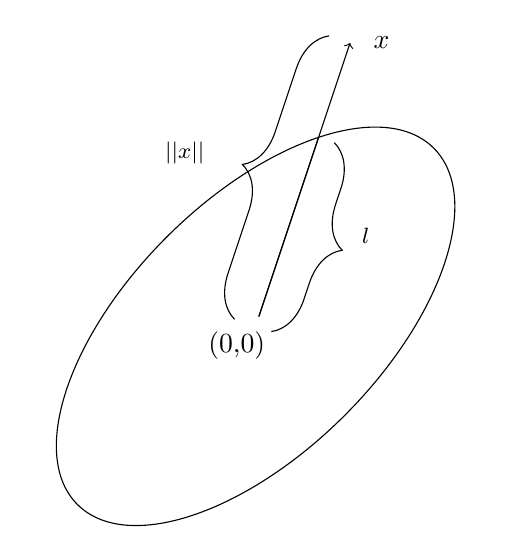
\begin{tikzpicture}[scale=0.8]
\draw  [rotate=45] (0,0) node (v1) {} ellipse (4 and 2);
\draw (v1) -- (1,3);
\draw [->] (v1) -- (1.5,4.5);
\draw [decorate,decoration={brace,amplitude=15pt,mirror,raise=6pt},yshift=0pt]
(0,0) -- (1,3) node [black,midway,xshift=1cm,yshift=-1.4] {\footnotesize
$l$};
\draw [decorate,decoration={brace,amplitude=15pt,raise=8pt},yshift=0pt]
(0,0) -- (1.5,4.5) node [black,midway,xshift=-1.5cm,yshift=0.4cm] {\footnotesize
$||x||$};
\node at (2,4.5) {$x$};
\node at (-0.3,-0.3) {(0,0)};
\end{tikzpicture}
}





\begin{document}

\title{BSc Project\\\textbf{Learning to Play Tetris using
    the Covariance Matrix Adaptation
    Evolution Strategy}}
\date{\today}
\maketitle

\tableofcontents

\clearpage

\begin{abstract}
We conduct an unbiased comparison between 
the Cross-entropy method and the Covariance Matrix Adaption
Evolution Strategy (CMA-ES) in training 
an agent to play the classical video game, Tetris. Many researchers have 
previously explored methods for constructing artificial Tetris
agents, but mostly focusing on how to maximize the score of the agents.
A common approach is to construct a configurable controller
and apply some optimization algorithm from the field of machine learning
to set the parameters for the best possible controller. Using the 
commonly used MDPTetris \citep{mdptetris} platform, the Cross Entropy
method is benchmarked against the CMA-ES algorithm under the same
conditions to reach an empirical understanding of how the two algorithms
compare when applied to Tetris. The results from our experiments
suggests that the Cross-entropy method is the preferable choice
between the two. They appear to reach similar scores, 
but the Cross-entropy method reaches this score almost twice as
fast as CMA-ES.
\end{abstract}

\begin{abstract}
Dansk Version
\end{abstract}



\section{Introduction \label{sec:intro}}

This thesis will cover an experimental approach 
to compare two optimization algorithms both considered 
state-of-the-art search methods. The algorithms addressed
are in particular known as the Cross Entropy method and 
the Covariance Matrix Adaption Evolution Strategy (CMA-ES
for short). The algorithms are each characterized by their
ability to search in rough multidimensional 
search spaces that only offers little possibility 
for analytical and deterministic approaches.
The algorithms will be applied to 
learning the game Tetris. Most often, when machine learning
techniques are applied to problems such as games, conventional
learning methods fall short due to both  very large number of 
possible actions in the games and highly unpredictable mappings 
between actions and their long-term consequences. The games 
are considered as episodic tasks where some agent is placed
in the game environment and interacts with the game following some
strategy that will hopefully result in a high score. 
The agent will make decisions on how to react 
to the game while playing, and optimizing the agent is hence a task of
finding good (as possible) policies for the agent to follow. Yet, as mentioned,
deciding what makes a policy good can be very difficult in
problems like games. When applying reinforcement methods to learning
the policies, conventional approaches typically do not suffice 
due to infeasible computation times. We will cover how
Tetris can be formulated in way that allows  the Cross-entropy method 
and CMA-ES to search for policies, and we will experimentally 
attempt to obtain an empirical perception of whether of the two algorithms
are preferable in this scenario.

\subsection{Reinforcement learning \label{RL}}

In the field of machine learning, the subfield of reinforcement learning
deals with training agents to behave in an environment through
trial and error. The environment typically consists of a set of states that cover all
scenarios the agent can encounter. The agent then has a set of actions
that it can use to make transitions between the states. 
The reinforcement learning methods relates somewhat 
to supervised models.
In supervised learning, every decision is tied to a predefined value
that defines how desirable the given action is. This way, in supervised learning,
the agent will always at any point have very detailed feedback signals from its actions.
In the context of actions and state transitions, an agent that learns trough
supervised learning will for every action taken know the absolute consequence
immediately after committing it.
Reinforcement learning is in many ways similar to supervised learning. 
The main difference between the two models is that agent does not receive 
an immediate response to its actions. Instead, the agent will receive a reward
when reaching certain states. The objective of the agent is then to
accumulate as much reward as possible. This differs from supervised learning
as the agent cannot know if reaching high amount of reward in the next state
will cause negative consequences in the future. Thus, the only decisive 
feedback given to the agent about its overall performance is 
how much cumulative reward it achieved at the end of a game.
In the game of Tetris, the reward is a direct mapping to 
the score achieved by the agent.
An example of how this two learning models apply to the simple game of
Tic Tac Toe. If supervised learning
is applied, the playing agent will for each move in the game know
if the move was considered desirable or not. 
In reinforcement learning however, only feedback the agent receives
is whether the games ended in a win, draw or a loose. Hence, the agent
cannot rely on signals during the game to adjust it's strategy.\\
\\
Often in the case of games, the 
time frame naturally falls into playthroughs in which the 
goal of the agent is to accumulate as much reward as possible 
before the game ends.
When the agent interacts 
with the environment, it uses a predefined set of actions
that each alters the state of the environment. In the case of 
Tic Tac Toe, the environment is the current state of the game, 
in terms of which markers are occupying spaces on the board.
The actions are the options to place a marker
on an empty space.
When deciding which action to carry out, the agent will use
a policy that maps the state of the environment to an action.
In Tic Tac Toe, a policy might be a table that has an entry for each possible
state of the board that maps to where the agent should place its marker.
The goal of the agent is then to choose a policy that maps states to actions 
in a way that
gives the highest possible cumulative reward at the end of a playthrough. 
Rewards in states can be negative and cause a 'penalty' to the agent if it reaches
such state. However, in the case of Tetris the agent cannot loose score,
and will therefore never be penalized.
Games often have a terminal state at which the game ends, which is 
also the case for Tetris and Tic Tac Toe. It's easy to see how the
Tic Tac Toe cannot last forever as it has 9 spaces, and for each turn in the game,
a space is occupied. However, the reason for why Tetris cannot play forever
lies within the fact that there exists a sequence of pieces that will
with certainty cause the player to loose, and if the player plays for 
long enough, this sequence will eventually occur. Thus, the agent must
attempt to acquire as much reward as possible before reaching the terminal 
state. 
When the agent chooses an action it cannot necessarily know what state
the action leads to, and in games this uncertainty is often present.
In Tic Tac Toe, the action taken by the agent will always with certainty 
lead to a known state, namely the board configuration where the marker is placed.
However, in Tetris, part of the state is the piece that is currently falling.
Thus, when the agent chooses a place to drop the piece, it has full control
over where to drop it, however it cannot decide what the next piece is. 
As there are 7 different piece
types in Tetris, each action can lead to 7 other states, each with a predefined probability.
It should also be noted that these probabilities for the individual transitions
must remain fixed across the entire playthrough of the game \citep{Carr}.
To find the best policy, there are a number of methods to pick from,
and the most obvious is a full traversal of the entire state space.
If one can afford to compute all rewards acquired from all possible 
actions in all possible states, one can choose the policy 
that gives the best cumulative reward. However, if the state space is
large, such computations become infeasible. The state space in Tetris
is indeed far too large to comprehensively walk through.
Due to this, one must use other ways of discovering good policies.
The methods used in reinforcement learning 
specify how the agent should change its policy according to 
results from earlier playthroughs, and the specific methods used in
the context of Tetris is explained in further detail in later sections.




\subsection{Learning Tetris \label{sec:learningTetris}}

On the topic of reinforcement learning, a widely used benchmark
for learning algorithms are designing agents 
for playing the classical video game of Tetris. Tetris is an 
appealing benchmarking problem due to it's complexity. The 
standard games plays on a board made from a grid that is
10 cells wide and 20 cells tall. As the game progress, differently
shaped pieces fall from the top of the board. 
When a row on the board is fully occupied by pieces, the line
is removed, all lines above it moved one line down and a score
point is given to the player. If a cell above the 20 rows first is
occupied, the game ends. The task of the player is to move
and rotate the falling pieces in a way that yields the highest 
score before the game ends.\\
\\
Tetris is indeed a hard task to computationally optimize, as
the game has a very high number of board configurations estimated to be
$10^{59}$ \citep{scherrer2009}. In relation to reinforcement learning,
an agent that plays Tetris is placed in an environment with a set of 
states far too large to exhaustively explore, and a set of transitions
that are stochastic. Because of this
complexity, a common approach 
in the literature is to use 
\textit{one-piece controllers}\footnote{Agents and controllers
both refer to artificial players.}, such as described in 
\cite{scherrer2009:b}. These controllers are only aware of
the current board state and the currently falling piece.
Hence, the policy of the agent is only to greedily choose
the action that transitions to the most rewarding state
from a single piece, which is typically less than 80 states\footnote{
Assuming 4 possible rotations and 20 columns
in which the piece may be dropped.}.
Using these controllers, the search space is reduced 
to only looking at the current board, and the possible 
places to drop the piece. \\
The game used for the benchmarking is a simplified version of Tetris,
in which 
controllers need only to decide in what column to drop the current
piece, and what orientation the piece should have when dropped.
Thus, the simplified version of Tetris differs from the 
original game mainly in two significant aspects. 
First, the controller is 
disallowed to move the piece horizontally while the piece 
is falling. Second, the controller has 'infinite'
time to make its decision on where to drop the current piece.
This way, the game only progress in discrete time steps
when the controller takes
an action, whereas the classical game runs continuously 
regardless of the players actions.
Thus, the controller cannot take advantage of moving the piece 
during the fall, but is not restricted by the time limitations.
This is however a common way of benchmarking Tetris playing agents
\citep{scherrer2009}\\
\\
When the controllers decide which action to take, it will
simulate each of the possible actions and choose the one that
leads to the most favourable board state. To evaluate the board 
state, the controller uses a set of features that defines 
various qualities of the board, and associate a weight to each 
feature. This means that the efficiency of the controller 
is determined by the features the controller is aware of
and how heavily they are weighted. This allows
the controller with $n$ features to be expressed as an 
$n$ dimensional real-valued vector, with one dimension 
per feature, and the value in that dimension the weight.
An often referred to controller is the Dellacherie's controller, 
as described in \cite{scherrer2009}. This controller
takes six features of the board into account, seen in table 
\ref{table:dellfeat} on page \pageref{table:dellfeat}. In relation 
to reinforcement learning, the policy of the agent is the feature set
combined with the weights of each feature. 
When using the \textit{one-piece controllers}, the policy remains 
the same during the episode, and the learning is based on updating
the policy from concluded games, rather than picking up on signals
that occur in the game as it plays.







\subsection{Goals of the thesis}

Both the Cross-entropy method and the CMA-ES have been used 
for learning Tetris with \textit{one piece controllers}, 
%but as mentioned, 
yet to our knowledge, only little effort has been put into 
comparing the two algorithms. This thesis will explore
how the two methods compare against each other under similar
conditions. Therefore, we will use a set of features for the 
Tetris controllers among those
commonly used, and compare how the two optimizing algorithms 
differ. The goal however is not to find a controller that 
outperforms existing controllers, but only to investigate 
how the Cross-entropy method and CMA-ES differs when learning Tetris
with similar configurations.\\
\\
In this thesis, we will explore how the two state-of-the-art
optimization algorithms, Cross-entropy method and CMA-ES, differ when 
applied to the task of playing Tetris.\\
\\
The Shark library \citep{shark08} contains a
working implementation of the CMA-ES 
algorithm. The Cross-entropy method 
is not present in the Shark library and thus, 
a part of the thesis is to implement it ourselves to resemble
the implementation in
the work of other researchers. To document the 
soundness of the implemented Cross-entropy method, 
we will replicate the experiment in \citep{scherrer2009} and 
verify that we obtain the similar results.
Then, we will benchmark CMA-ES and the Cross-entropy method against each other 
to determine if one yields better optimization results than the other.


\subsection{Scope and limitations \label{section:scope}}


The experiments will be carried out on the simplified version of
Tetris using the MDPTetris software found at \citep{mdptetris},
which is the same simulator used by Scherrer et al. in \citep{scherrer2009:b} 
among other authors in various papers.
This software already have the well known feature sets
implemented, so we will not ourselves extend any of the features.
The source code of the Tetris simulator is used as-is, and is therefore 
not altered prior to running the experiments. 
For comparing the optimizers, the \shark library will be used. 
This library already contains an
implementation of the CMA-ES optimizer, but lacks the 
Cross-Entropy. Therefore, a part of this thesis will
be to implement and document the Cross-Entropy method in Shark.









\section{Background}


\subsection{Previous work \label{prevWork}}
Over the time, numerous researchers has tried different feature 
sets and applied various optimizers to find the best 
possible Tetris controllers. Researches in the field
of reinforcement learning have approached the task of learning Tetris
in various ways. Some have implemented exact versions of the original game
where the artificial Tetris player will have to interact with the 
game much like a human player. In these games the state of the board is not limited
to just the board configuration and the current piece, but also where in the 
board the piece is located. Hence, these controllers does not model actions 
as locations to drop the piece, but rather 'button presses' that controls the
fall of the piece. Yet, from the literature we have read, the most commonly applied 
type of controller is the one used in the MDPTetris platform. As mentioned earlier,
to create an efficient controller one can adjust two settings, namely the featureset 
and the associated weights. 
The specifics of how to tune the weighting is a topic that is 
explored along with finding the feature sets themselves. A common 
feature set, the Dellacherie feature set (see figure \ref{table:dellfeat}),
was originally tuned by hand with trial and error approach with a surprisingly 
good result. Yet, the most common approach is to apply some optimization 
algorithm to adjust the weighting.
The features used are typically
ones that attempt to mimic the board conditions that would
normally catch the attention of a human player, such as
how high the overall pile of pieces is and how many holes 
the board has. In \citep{scherrer2009:b} table 1, a table 
presents some feature sets used throughout various publications
on the subject. The feature sets applied in this thesis are 
Dellacherie and the Bertsekas feature sets 
(see figure \ref{table:dellfeat} and \ref{table:bertfeat}) due 
to their recurring usage across various articles.
Many authors have had success
with applying evolutionary stochastic search methods for tuning 
the weights of the feature sets towards
efficient controllers. However, the goal of most research 
is to outperform existing controllers and push the boundaries
of performance when learning Tetris. This means that the objective of
these researchers is often to craft feature sets that perceives the 
board in a way that allows the agent to make the best possible decisions.
Thus the focus in most works is combined on finding good feature sets and 
finding good ways to optimize the weights of the set. In this thesis,
our goal is not to find a controller that outperforms any existing one,
but rather to investigate the learning properties of the optimization algorithms.
For this purpose
we are in particular addressing the
Cross-Entropy method described in detail in \citep{cetut2014} and the
Covariance Matrix Adaption Evolution Strategy (CMA-ES), described 
in \citep{hansen2011}. The particular Cross-Entropy method applied 
is the one described in \citep{szita:06} as the "Noisy Cross Entropy Method".\\

\begin{figure}[h!]
\begin{center}
\begin{tabular}{| l | p{8cm} |}
\hline
\textbf{Feature} & \textbf{Description}\\
\hline
Landing height & The height of the last piece when it was placed\\
\hline
Eroded piece cells & Number of rows cleared in the last move
times the number of bricks cleared from the last move\\
\hline
Row transitions & Number of horizontal cell transitions\\
\hline
Column transitions & Number of vertical cell transitions \\
\hline
Holes & Number of empty cells covered by a full cell\\
\hline
Board wells & Cumulative sum of cells to the depth of
the board wells.\\
\hline
\end{tabular}
\end{center}
\caption{features of the Dellacherie featureset \label{table:dellfeat}}
\end{figure}

\begin{figure}[h!]
\begin{center}
\begin{tabular}{| l | p{8cm} |}
\hline
\textbf{Feature} & \textbf{Description}\\
\hline
Max height & Height height of the highest occupied block\\
\hline
Column height & Height of each column\\
\hline
Height difference & The height difference between columns\\
\hline
\end{tabular}
\end{center}
\caption{features of the Dellacherie featureset \label{table:bertfeat}}
\end{figure}


Currently, many researchers have proposed numerous 
feature sets and multiple 
optimization methods have been explored. 
The Dellacherie controller is very widely used across many resources
\citep{fahey}. This controller was hand-tuned by trial and error,
and did originally, on a regular non-simplified Tetris game, achieve an average of
660 000 lines. The same feature set (see figure \ref{table:dellfeat}) is 
often incoorporated in later works when optimizing controllers. An earlier
feature set is the set proposed by \citep{Bertsekas} referred to as Bertsekas and
Tsitsiklis features. In 2006, Szita and L\H{o}rincz \citep{szita:06} applied the Cross-Entropy
method using the Bertsekas and Tsitsiklis features. They report that using no noise,
their controller converged at 300 000 lines on average. 
The best result reported in \citep{szita:06}
is when decreasing noise is applied, 
in which the controller's score exceeded 800 000 lines. 
However, in a later paper, using Dellacherie, 
Bertsekas and two selfdefined features achieved 
35.000.000 lines $\pm 20\%$  \citep{scherrer2009}.\\




\input{Background/objectiveFunction}

\subsection{Optimizers \label{Optimizers}}

In this thesis, the Cross-Entropy method and the Covariance Matrix Evolution 
Strategy are compared. Both of the methods fall into the category of 
\textit{stochastic optimization}
methods. These methods are useful for 
optimization problems where the gradient is not available.
The optimization functions aim to optimize 
the parameter set $\textbf{\individual }$
for the objective function $\fitnessFunction$.
\begin{align}
\hat{\textbf{\individual }} &= 
arg \  \underset{\textbf{\individual }}{max} \  
\fitnessFunction (\textbf{\individual }) \ 
:\mathbb{R}^{\dimensions } \rightarrow \mathbb{R}
\end{align}

In these methods, the optimizing algorithm uses a family of parametric distributions,
and maintains a mean $\mean $ along with other parameters
to search the best possible solution for the objective function.  
In the case studied in this thesis
both the CMA-ES and Cross-entropy methods use a 
Gaussian distribution to sample solutions to the objective function.
Hence, both of the functions aim to find a mean 
$\mean $ and an $\dimensions \times \dimensions$ matrix 
$\varianceMatrix $\footnote{In \citep{hansen2011}, 
$\sigma$ is used for step-size in CMA-ES, so $\varianceMatrix $ is instead introduced
as an arbitrary $\dimensions \times \dimensions$ matrix in its place.}, such that when
a vector $\textbf{\individual }$ is sampled by 
$\textbf{\individual } \sim \mathcal{N}\left( \mean, \varianceMatrix \right)$, 
then $\fitnessFunction (\textbf{\individual })$ 
is likely to yield preferable results.\\
\\
The algorithms work iteratively, such that the mean and variance 
of the distribution 
is altered for each iteration $\generation $.
The algorithms start by initializing the 
parameters either at random or at some fixed point. A common 
configuration is setting the mean to 
all zeros and the standard deviation to the identity matrix.
Thus, for the first iteration $\generation = 0$, a configuration could be:
\begin{align}
\mean^{(0)} =
\begin{bmatrix}
0\\
\vdots\\
0
\end{bmatrix},\ \ 
\varianceMatrix^{(0)} = 
\begin{bmatrix}
1 & \hdots & 0\\
\vdots & \ddots & \vdots\\
0 & \hdots & 1
\end{bmatrix}
\end{align}

The superscript of $(0)$ notes that the values occur in iteration 0.\\
\\
In each iteration, the algorithms sample $\populationSize$ candidate solutions 
and evaluate their fitness
against the objective function. When each of the solutions are evaluated,
they are ordered according to their fitness:
\begin{align}
\{\textbf{\individual }_{1}, \hdots, 
\textbf{\individual }_{\populationSize }\}\ \ \text{Such that}\ \ 
\fitnessFunction(\textbf{x}_1) \geq 
\fitnessFunction(\textbf{\individual }_2), \hdots, 
\fitnessFunction(\textbf{\individual }_{\populationSize  - 1}) \geq 
\fitnessFunction(\textbf{\individual }_{\populationSize })
\end{align}

The mean and standard deviation for the next iteration, 
that is $m^{(\generation+1)}$ and $M^{(\generation+1)}$, are
then updated usually by considering the best of the ordered solutions. How exactly
these parameters are updated is individual for each method and can be seen in the following
sections.




\subsection{CE (Cross Entropy) \label{CrossEntropy}}
CE is described through many papers in 
slightly different ways. This section
describes the algorithm in a similar fashion 
to \citep{thiery:09}.\\
\\
This method uses a Gaussian distribution to 
sample sample vectors for the objective function
$\fitnessFunction$. The algorithm aims to 
adjust the parameters of the distribution
such that samples $\individual$ drawn from the distribution
gives the best possible results when applied to the
objective function $\fitnessFunction \left( \individual \right)$.\\
\\
The Cross-Entropy method starts with an initial 
mean $\mean$ which is an $n$-dimensional vector
typically set to 0
\begin{align}
\mean^{(0)} = \begin{pmatrix}
0\\
\vdots\\
0
\end{pmatrix} 
\end{align}

The second argument to the gaussian distribution is a 
diaginal matrix which contains the variance for each 
component

\begin{align}
\varianceMatrix^{(0)} =
\begin{bmatrix}
\sigma_1^{2} & \hdots & 0\\
\vdots & \ddots & \vdots\\
0 & \hdots & \sigma_{\dimensions}^{2}
\end{bmatrix}
\end{align}
The algorithm will in each generation sample a set of search points
and rank these using the objective function.
In each generation, $\populationSize$ vectors are sampled by 
$\individual_{i} \sim \mathcal{N} \left(\mean, \varianceMatrix^{2} \right)
,\ i \in \{1,\dots,\populationSize \}$. The vectors are all evaluated 
against the fitness function and ordered such that $\fitnessFunction \left( \individual_{1} \right) \geq, \dots, \geq \fitnessFunction \left( \individual_{\populationSize} \right)$
, and the $\offspringNumber$ best are chosen for updating the distribution 
parameters. The mean is updated as the centroid of the chosen vectors, and
the variance in each dimension is set to the variance of the chosen vectors in each 
dimension.\\

The pseudo code and details of the algorithm can be seen in figure
\ref{fig:ceCode} on page \pageref{fig:ceCode}.

\begin{figure}[H]
\hrule
\vspace{0.2cm}
{\centering  \textit{Noisy cross-entropy method}}
\vspace{0.2cm}
\hrule
\begin{algorithmic}
\State{\textbf{input}}
\State{$\fitnessFunction$ : The function that estimates the performance of a vector $\individual$}
\State{($\mean^{(0)}$, $\varianceMatrix^{(0)}$): The mean and variance of the initial distribution}
\State{$\populationSize$ : The number of vectors sampled per generation/iteration}
\State{$\offspringNumber$: The number of offspring selected for the new mean}
\State{$\noise_{\generation}$: The noise added to each generation/iteration}
\\

\Loop
\State{Generate $\populationSize$ vectors $\individual_{1}, \individual_{2}, \dots, \individual_{\populationSize}$ from $\mathcal{N}(\mean^{(\generation)}, \varianceMatrix^{(\generation)})$}
\State{Evaluate each vector using $\fitnessFunction$}
\State{Select the $\offspringNumber$ vectors with the highest evaluation}
\State{Update $\mean^{(\generation + 1)}$ based on the $\offspringNumber$ best vectors}
\State{Update $\varianceMatrix^{(\generation + 1)}$ based on the $\offspringNumber$ best vectors + $\noise^{(\generation)}$}
\EndLoop
\end{algorithmic}
\hrule
\caption{The pseudo code for the Cross-Entropy algorithm \label{fig:ceCode}}
\end{figure}

\subsubsection{Input}

\textbf{The objective function \label{CEObjective}} \\
The objective function $\fitnessFunction$ is a 
function used to rank the value of a sampled vector.
As described in the 'Optimizers' section, CE is a general stochastic 
iterative algorithm that tries to solve an optimization problem of 
the form \citep{thiery:09}:
\begin{align}
\hat{\textbf{\individual }} &= 
arg \  \underset{\textbf{\individual }}{max} \  
\fitnessFunction (\textbf{\individual }) \ 
\end{align}
Where $x$ corresponds to a given vector, 
and $\fitnessFunction$ is our actual objective function. 
\\

\textbf{The mean and variance of the gaussian distribution} \\
Here $\mean^{(\generation)}$ is the mean and  
$\varianceMatrix^{(\generation)}$ is the covariance matrix, with 
the variance in each dimension along the diagonal, and zeros elsewhere. 
The parameters in the Gaussian distribution are ($\mean^{(\generation)}$,
$\varianceMatrix^{(\generation)}$). 
More specifically this Gaussian distribution is defined as 
\begin{align}
\mathcal{N}(\mean^{(\generation)},\varianceMatrix^{(\generation)})
\end{align}

Where $\generation$ denotes the current iteration.\\


\textbf{The number of vectors}\\
$\populationSize$ is the number of vectors sampled in each generation.
\\

\textbf{The number of selected vectors / parents}\\
$\offspringNumber$ is the number of vectors which are selected to compute 
the new mean $\mean_{\generation + 1}$, and variance
$\varianceMatrix^2_{\generation + 1}$, for next generation/iteration. 
These offspring vectors gets selected 
directly by taking the $\offspringNumber$ best ranked
vectors.
\\

\textbf{The noise term}\\
The noise factor, $\noise_{\generation}$, 
is the amount of noise which 
is applied to the variance $\varianceMatrix^2$ in
iteration/generation 
$\generation$. In general, noise is used to prevent
the algorithm from 
getting narrowing down to an undesired local optimum, but
rather explore new solutions.
The noise term can be any
function of $\generation$. Among 
the most described noise types are: no noise, constant noise 
and linear decreasing noise \citep{szita:06}. 
When using no noise, $\noise_{\generation}$ 
is simply set to zero. When using constant noise, 
the same value is 
added to the variance $\varianceMatrix^2$ 
in each iteration/generation. 
When using linear decreasing noise, 
$\noise_{\generation}$ is often set as
$\noise_{\generation}=max(5- \generation /10,0)$.
\\

\subsubsection{Loop}

\textbf{Sampling the population}\\
The first step of the loop is to generate the new generation 
consisting of $\populationSize$ vectors. 
These vectors are drawn from the distribution 
$\individual_{i}\sim \mathcal{N}(\mean_{\generation},\varianceMatrix^2_{\generation})$.
\\

\textbf{Evaluating the population}\\
After sampling the population, the algorithm needs to order the vectors to find the $\offspringNumber$ best vectors, each vector $\individual_{i}\ ,\ i \in \{1, \dots, \populationSize\}$ is evaluated using $\fitnessFunction$. 
The value from the objective function then yields 
the estimated performance of each individual.
\\

\textbf{Selecting the parents}\\
As each $\individual_{i}$ has an assigned evaluation value, and the 
$\offspringNumber$ best vectors gets selected by 
taking the $\individual_{i}$ vectors with the highest ranking.
\\

\textbf{Updating the distribution parameters}\\
When updating the distribution parameters for the next iteration
($\mean^{(\generation + 1)}$,$\varianceMatrix^{(\generation + 1)}$), 
the mean is updated by computing the centroid of the 
$\offspringNumber$ highest ranking vectors. This is formally defined as:
\begin{align}
\mean^{(\generation +1)}:=\frac{\sum_{i=1}^{\offspringNumber} \individual_{i}}{\offspringNumber}
\ \ \ 
\text{where}
\ \ \ 
\fitnessFunction \left( \individual_{1} \right) \geq, \dots, 
\geq \fitnessFunction \left( \individual_{\offspringNumber} \right) \geq, 
\dots, \geq \fitnessFunction \left( \individual_{\populationSize} \right)
\end{align}
The diagonal matrix of variances $\varianceMatrix^{(\generation + 1)}$ is updated 
to match the variance of the $\offspringNumber$ best
vectors, such that the variance in dimension $k$ 
matches the variance of the $\offspringNumber$
in dimension $k$. Hence, for $k \in \{ 1,\dots,\dimensions \}$,
the $(k,k)$'th entry in the variance matrix is 
updated 
This is formally defined as:
\begin{align}
{\varianceMatrix^{(\generation +1)}}_{k,k}:=\frac{\sum_{i}^{\offspringNumber}
({\individual_{i}}_k - \mean_{\generation +1})^2}{\offspringNumber} + 
\noise_{\generation + 1}\ ,\ \ k \in \{ 1,\dots,\dimensions \}
\end{align}

\subsection{CMA-ES \label{CMAtheory}}


This description is based on the tutorial written by Nikolaus Hansen
\citep{hansen2011}. This section will not focus on the theoretical derivation
of CMA, but rather how it deviates from Cross Entropy. 
The CMA operates on a general level much like the Cross Entropy 
method, but includes some features that increases the adaptability 
of the algorithm.\\
\\
The CMA, like the Cross Entropy, uses a Gaussian distribution to
search for good solutions to $\fitnessFunction$. Yet, for the 
variance parameter, the CMA provides a full covariance matrix.
As the Cross Entropy method only provides a diagonal matrix of scalers,
it's restricted to only scaling the ellipsoid of equal density along
the coordinate axes. The CMA however, with a full covariance matrix,
allows the ellipsoid to rotate arbitrarily in the search space.\\
Another difference between the two algorithms is that 
Cross Entropy only considers the next population when updating the
distribution parameters, while the CMA keeps track of 
some information from earlier 
generations. This allows the CMA somewhat keep track of the evolution 
of the sampled vectors.\\
The CMA also differs from Cross Entropy in how it evaluates the influence 
of the parent vectors. As Cross Entropy weights all vectors equally when 
moving the mean. The CMA, at least from the implementation in SHARK, 
has the option of taking a weighted combination of the offspring in order
to bias towards the better vectors.

\begin{figure}[H]
\hrule
\vspace{0.2cm}
{\centering  \textit{CMA-ES}}
\vspace{0.2cm}
\hrule
\begin{algorithmic}
\State{\textbf{input}}
\State{$\fitnessFunction$: The function that estimates the performance of a vector $\individual$}
\State{($\mean$, $C$): The mean and variance of the initial distribution, where 
$C$ is the covariance matrix usually set to $C=I$}
\State{$\lambda$: The number of vectors sampled per generation/iteration}
\State{$\offspringNumber$: The number of offspring selected for the new mean}
\\
\State{\textbf{initialization}}
\State{Set initial internal parameters}
\\
\Loop
\State{Increment generation counter2}
\State{Sample new generation}
\State{Evaluate each vector using $\fitnessFunction$ and recombine}
\State{Covariance matrix adaption}
\State{Step-size control}
\EndLoop
\end{algorithmic}
\hrule
\caption{The pseudo code for the Cross-Entropy algorithm \label{fig:cmaCode}}
\end{figure}

Note here that the population size in this section is denoted as
$\lambda$ as opposed to $\populationSize$. Also the iteration/generation 
counter is referred to s $g$ rather than $\generation$. 
This is to remain consistent 
with the tutorial.

\subsubsection{Input}

\textbf{The objective function} \\
This serves the same purpose as in Cross Entropy (see page \pageref{CEObjective}).
\\

\textbf{The mean and variance of the gaussian distribution} \\
Here $\mean^{(g)}$ is the mean and  
${C^{(g)}}^{2}$ is the variance 
of the gaussian distribution ($\mean^{(g)}$,
${C^{(g)}}^2$). 
More specifically this gaussian distribution is defined as 
\begin{align*}
\mathcal{N}(\mean_{\generation},\sigma C^2_{\generation})
\end{align*}

Where $g$ denotes the current iteration/generation.\\


\textbf{The number of vectors}\\
$\populationSize$ is the number of vectors sampled in each generation.
\\

\textbf{The number of offspring}\\
$\offspringNumber$ is the number of vectors which are used to compute 
the new mean very much like in Cross Entropy. However the CMA algorithm
is not bound to weight each vec tor equally. It has the option to assign 
a weight to each vector and hence biasing towards the better solutions.
\\


\subsubsection{Initialization}


Set parameters
\begin{align}
\lambda, \offspringNumber, w_{i \dots \offspringNumber}, c_{\sigma}, d_{\sigma}, c_c, c_1, c_{\offspringNumber}
\end{align}
To their default values according to table 1 in \citep{hansen2011}.

Set evolution path $p_{\sigma} = 0$, $p_{c} = 0$, covariance matrix $C = I$ and $g = 0$

Where:

\begin{align}
\lambda, \mu, g &\in \mathbb{N}\\
w_i,\dots,w_{\mu}, c_{\sigma}, d_{\sigma}, c_c, c_1, c_{\lambda}, &\in \mathbb{R}\\
p_{c}, p_{\sigma} &\in \mathbb{R}^{\dimensions}\\
C &\in \mathbb{R}^{\dimensions \times \dimensions}
\end{align}

Again, note that $\lambda$ has the meaning of $\populationSize$ from earlier, that
is $\lambda$ is in this case the population size. $\mu$ however, is still the number
of vectors that contribute to the updating of distribution parameters, namely the 
parent size.\\
\\
In this algorithm, the distribution used is multivariate normal distribution defined
as 
\begin{align}
\mathcal{N} \left( m,  \sigma^2 C \right)
\end{align}
This distribution describes the set of correlated real-valued vectors that
clusters around the mean vector $m$ and has a covariance described by the
matrix $C$. The covariance matrix describes the 'shape' of the space in which 
the vectors are most likely to be sampled. For illustrative purposes,
the shape of the sampling space is drawn as an ellipseoid.
This ellipoid depicts a set of points that has equal denity 
in the probability denisty function of $C$, and is hence refered to 
as the ellipse of equal density.
With a covariance matrix $C$
the ellipsoid is defined as points that stisfies
$\{x \in R^{\dimensions} | x^{T} C^{-1} x = 1\}$.
When illustrating this, the step-size is set as $\sigma = 1$ for simplicity.\\
\\
The matrix $C^{-1}$ is decomposed as $C^{-1} = B D^{-2} B^T$, where $B$ is a rotation 
matrix that rotates from the coordinate axises into the principal axises of $C$, and 
$D^{-2}$ is the diagonal matrix 
$\text{diag} \left( \frac{1}{d_{1}^2},\dots, \frac{1}{d_{\dimensions}^2} \right)$
where $d_{i}$ is the $i$'th eigenvalue of $C$. Figure \ref{fig:ellipse} shows an example
of how to determine if a point lies on the ellipsoid. In this example, the aim is to 
determine if the point $x$ lies on the two-dimensional ellipsoid, hence checking if 
$x^{T} C^{-1} x = 1 \Leftrightarrow x^{T} B D^{-2} B^T x = 1 $ holds. In figure 
\ref{fig:ellipse}, $l$ is the length from the origin of the ellipse to the edge.
Consider the operation
\begin{align}
B D^{-2} B^T x \label{eq:rotscal}
\end{align}

The order of operations are the following. 
$B^{T}$ rotates $x$ from the principal axises of $C$
into the coordinate axises. Then $D^{-2}$ scales the point by $\frac{1}{l^2}$ where
$l$ is the length from the ellipsoid origin to the edge. Finally, $B$ rotates the point 
back in the original direction. thus, (\ref{eq:rotscal}) has the same effect as
\begin{align}
\frac{1}{l^2} x
\end{align}
Hence, the entire operation is equivalent to
\begin{align}
x^{T} B D^{-2} B^T x &= x^{T} \frac{1}{l^2} x = \frac{1}{l^2} x^{T} x
= \frac{1}{l^2} ||x||^2
\end{align}
This means that if $||x||^2 = l^2$ then $x$ lies on the ellipse.
In the example of figure \ref{fig:ellipse}, $x$ is not 
on the ellipse.


\begin{figure}[H]
\begin{center}

\end{center}
\begin{center}
\ellipseFigure
\end{center}
\caption{Illustration of $\{x \in R^{\dimensions} | x^{T} C^{-1} x \stackrel{?}{=} 1\}$ \label{fig:ellipse}}
\end{figure}

\subsubsection{Loop}

\textbf{Increment iteration counter}

If the stopping criteria is not met
\begin{align}
g &= g+1
\end{align}
Otherwise, stop.\\


\textbf{Sample new generation}\\
Sample new population of search points, for $k = 1, \dots, \lambda$.
The aim is to sample vectors in the following form
\begin{align}
\individual_{k} \sim \mathcal{N}(m, \sigma^2 C)
\end{align}


To generate the sample for the generation, the covariance matrix is first 
decomposed using principal component analysis into
\begin{align}
C = B D^2 B^{T}
\end{align}

Where $B = \begin{bmatrix}
b_1, & \dots, & b_\dimensions
\end{bmatrix}$ 
is am orthogonal basis of eigenvectors, and  
$D = \text{diag}\left(d_1, \dots, d_\dimensions\right)$
is a diagonal matrix that contains all eigenvalues of $C$.\\
\\
Intermediately, the vectors are sampled from a Gaussian distribution 
with zero mean and
the identity matrix as variance.
\begin{align}
z_{k} &\sim \mathcal{N}(0, I)
\end{align}

$z_k$ is then multiplied by a factor that causes the them to form 
after the covariance matrix $C$. From Hansens tutorial, it's derived that
\begin{align}
C^{-1} &= B D^{-2} B^{T}\\
C^{\frac{1}{2}} &= B D B^{T}
\end{align}

Thus, to get the effect of the covariance matrix to apply to the $z_k$
samples, the following is used

\begin{align}
\mathcal{N}\left( 0, C \right) \sim C^{\frac{1}{2}} \mathcal{N}\left( 0, I \right)
\end{align}

\begin{align}
y_{k} &= B D \underbrace{B^{T} z_{k}}_{\sim \mathcal{N}(0, I)} \sim \mathcal{N}(0, C)\\
y_{k} &= B Dz_{k} \sim \mathcal{N}(0, C) \label{eq:sampley}
\end{align}

$B$ is the orthogonal basis of vectors of unit length, which means that 
$B$ is purely a rotation matrix. Due to this, $B^{T} z_{k}$ only rotates
$z_k$ yielding the same distribution. After this, the $BD$ is multiplied,
which applies the scale such that each vector is scaled to match the
variance in the principal axises of the covariance matrix, and $B$ 
will rotate each sample such that it aligns with the principal axises
of $C$. After this step, $y_{k}$ now resemble the vectors that rotated and scaled
to match shape of the covariance matrix.\\

The mean and step-size $\sigma$ is applied.
\begin{align}
x_{k} &= m + \sigma y_{k} \sim \mathcal{N}(m, \sigma^2 C) \label{eq:finalSample}
\end{align}



Finally, the $x_{k}$ vector resemble a realization of the Gaussian distribution
with mean $m$ and covariance matrix $C$ scaled by the step-size $\sigma$.
Am illustration of the sampling process in two dimensions can be seen in figure \ref{fig:sampleing} where 
\begin{align}
\sigma = 1,\ B = \begin{bmatrix}
{b_1}_x & {b_2}_x\\
{b_1}_y & {b_2}_y
\end{bmatrix},\ D = \begin{bmatrix}
d_1 & 0\\
0   & d_2
\end{bmatrix}
\end{align}


\begin{figure}[H]
\begin{center}
\begin{tabular}{c c c}
\begin{tikzpicture}[scale=0.5]
\draw [->] (0,-5) -- (0,5);
\draw [->] (-5,0) -- (5,0);
\node at (0,0) {};
\draw  (0,0) ellipse (2 and 2);
\draw (0,0) -- (2,0);
\draw [decorate,decoration={brace,amplitude=5,raise=2},yshift=0pt]
(0,0) -- (2,0) node [black,midway,xshift=0,yshift=15] {1};
\end{tikzpicture} &
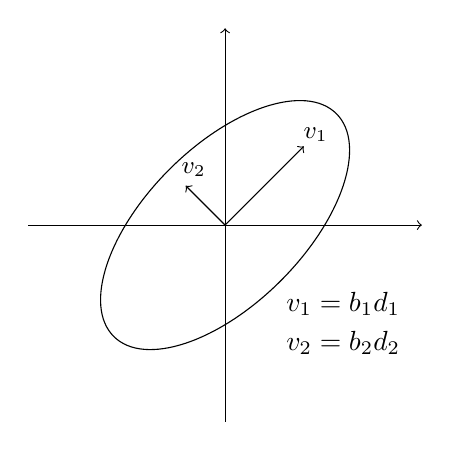
\begin{tikzpicture}[scale=0.5]
\draw [->] (0,-5) -- (0,5);
\draw [->] (-5,0) -- (5,0);
\node at (0,0) {};
\draw [rotate=45] (0,0) node (v1) {} ellipse (4 and 2);
\draw [->] (0,0) --  (2,2);
\draw [->] (0,0) -- (-1,1);
\node at (-0.8,1.4) {\small $v_2$};
\node at (2.3,2.3) {\small $v_1$};
\node at (3,-2) {$v_1 = b_1 d_1$};
\node at (3,-3) {$v_2 = b_2 d_2$};
\end{tikzpicture} &
\begin{tikzpicture}[scale=0.5]
\draw [->] (0,-5) -- (0,5);
\draw [->] (-5,0) -- (5,0);
\node at (1,1) {};
\draw [rotate=45] (1.5,0) node (v1) {} ellipse (4 and 2);
\draw [->](1,1) -- (3,3);
\draw [->] (1,1) -- (0,2);
\draw [fill] (1,1) ellipse (0.1 and 0.1);
\node at (2,1) {\small $m$};
\end{tikzpicture}\\
$z_{k} \sim \mathcal{N}(0, I)$ & $y_{k} \sim B Dz_{k}$ & $x_{k} \sim m + \sigma y_{k} \sim \mathcal{N}(m, \sigma^2 C)$
\end{tabular}
\end{center}
\caption{The steps of the sampling process \label{fig:sampleing}}
\end{figure}


\textbf{Evaluate each vector using $\fitnessFunction$ and recombine}\\
As each vector is evaluated, they are ranked such that
$\fitnessFunction{ \left( \individual_{i} \right) } \geq \dots \geq \fitnessFunction{ \left( \individual_{\offspringNumber} \right)} \geq \dots \geq \fitnessFunction{ \left( \individual_{\lambda} \right)}$.

\begin{align}
\langle y \rangle_{w} &= \sum^{\offspringNumber}_{i = 1}w_{i} y_{i : \lambda}
\end{align}

Where the notion of $y_{i : \lambda}$ means the $i$'th element in ranked list of vectors
where $y_1$ is the best ranked vector.

\begin{align}
\sum^{\offspringNumber}_{i = 1} w_{i} = 1, w_{i} > 0
\end{align}

$\langle y \rangle_{w}$ is a measure of a 'weighted center of mass',
and is part of the selection mechanism. The idea is to allow the selected vectors
to contribute differently to the update, and hence emphasize the higher 
ranking vectors. The individual weights are as the following

\begin{align}
w_i &= \frac{w_{i}'}{\sum^{\offspringNumber}_{j=1} w_j }
\end{align}

Where the $w_i'$ is used for a intermediate weighting value for the vectors.\\
In the Shark library, three built-in weighting types are implemented, each with
a distinct intermediate weight.

\begin{align}
\text{Equal}: &\quad w_i' = 1 \label{eq:recomType}\\
\text{Linear}: &\quad  w_i' = \offspringNumber - i\\
\text{Superlinear:} &\quad w_i' = ln \left( \offspringNumber + \frac{1}{2} \right)
- ln \left( i \right)
\end{align}
Thus, with the equal, each vector contributes equally, and with the other two, the 
higher ranking vectors has more influence on location of the 'center of mass' of 
the selection.

The new mean is computed as
\begin{align}
m^{(g+1)} &= m^{(g)} + \sigma \langle y \rangle_{w} = \sum^{\offspringNumber}_{i = 1} w_{i}x_{i:\lambda} \label{eq:movemean}
\end{align}
Such that the mean moves towards the 'center of mass' scaled by the step-size.
The details of step-size $\sigma$ is covered later in this section,
however in brief terms the step-size is meant to scale movements 
of the mean and the distribution area.\\
\\
In relation to the selection mechanism, the value $\mu_{eff}$ is introduced.
This is defined as
\begin{align}
\meff = \left( \sum_{i=1}^{\offspringNumber} w_i^2 \right)^{-1}
\end{align}
Hence $1 \leq \meff \leq \mu$. As an example, for the equal recombination
type, $\meff = \left( \sum_{i=1}^{\offspringNumber} w_i^2 \right)^{-1} = 1^{-1} =1$
In the tutorial by N. Hansen, it's mentioned that $\meff \approx 
\frac{\lambda}{4}$ indicates a good setting of $w_i$. The $\meff$ is 
measure of how much of the parent mass is used, and serves as a normalization 
factor in later equations.\\

\textbf{Covariance matrix adaption}

The idea of using the covariance matrix is to make new samples
resemble the covariance of the previous well-performing vectors, as opposed 
to the Cross Entropy algorithm that does not maintain any information of
previous samples.\\
\\
A evolution path of the movement of the means is introduced as $p_{c}$. This 
is a vector that holds the direction in which the mean has been moved in 
both the current generation, and in previous generations in 
a 'low-pass filter' like manner. Using the 
evolution path, the covariance matrix can take a shape that 
makes samples more likely to appear in the direction of successive 
movements of the mean.
The evolution path for generation $g+1$ is updated as

\begin{align}
p_{c}^{(g+1)} &= \underbrace{\left( 1 - c_{c} \right) 
p_{c}^{(g)}}_{\makebox[0pt]{\text{previous steps}}}  + 
\overbrace{h_{\sigma}}^{\makebox[0pt]{\text{{indicator function}}}}
\underbrace{\sqrt{c_{c} \left( 2 - c_{c} \right) \offspringNumber_{\text{eff}}}}_{
\makebox[0pt]{\text{normalization}}
}
\langle y \rangle_{w} \label{eq:epathc}
\end{align}
In (\ref{eq:epathc}), the term $\left( 1 - c_{c} \right) p_{c}^{(g)}$ makes 
the evolution path become influenced by earlier path steps. The learning rate
$c_c \in [0;1] $ indicates how much of the previous path is taken into account.
if $c_c = 0$, the previous path is not considered at all, and if $c_c = 1$ the path 
will only consist of the previous step. According to the tutorial, this is set
$c_c = \frac{4 + \mu_{eff} / \dimensions}{\dimensions + 4 + 2 \mu_{eff} / \dimensions}$.\\
\\
Th indicator function $h_{\sigma}$ is discussed in detail in the tutorial \citep{hansen2011}.
However, the main idea of this indicator function is.
\begin{align}
h_{\sigma}
\begin{cases} 1\ \ \ \text{if $||p_{\sigma}||$ is large} \\
              0\ \ \ \text{otherwise} %
\end{cases}
\end{align}
The purpose of this is to stall updating the evolution path when 
the length of the step-size evolution path becomes too large. The step-size
evolution path is covered in \textit{Step-size control}.\\
\\
The normalization factor 
$\sqrt{c_{c} \left( 2 - c_{c} \right) \offspringNumber_{\text{eff}}}$ is chosen such that
$p^{(g+1)}_{c} \sim \mathcal{N}\left(0, C \right)$ if $p_c^{(g)} \sim \mathcal{N} 
\left(0, C\right)$\\
To see that this holds, note that
\begin{align}
\langle y \rangle_{w} &= \frac{m^{(g+1)} - m^{(g)}}{\sigma}
\sim \frac{1}{\sqrt{\meff}}  \mathcal{N}\left(0, C \right)
\end{align}
\\
Thus, with the indicator function set aside
\begin{align}
p_{c}^{(g+1)} &\sim \left( 1 - c_{c} \right) 
\mathcal{N}\left(0, C \right) + 
\sqrt{c_{c} \left( 2 - c_{c} \right) \offspringNumber_{\text{eff}}}
\frac{1}{\sqrt{\meff}}\mathcal{N}\left(0, C \right) \label{eq:nomalization_start}\\
&\sim
\mathcal{N}\left(0, \left( 1 - c_{c} \right)^2 C \right) + 
\mathcal{N}\left(0, c_{c} \left( 2 - c_{c} \right)  C \right)\\
&\sim
\mathcal{N}\left(0, \left( 1 - c_{c} \right)^2 C + c_{c} \left( 2 - c_{c} \right)  C  \right)\\
&\sim \mathcal{N}\left( 0, C \right) \label{eq:nomalization_end}
\end{align}
Hance, the evolution path ios updated unbiased udner random selection.
\\
The covariance matrix is updated as follows
\begin{align}
C^{(g+1)} &= 
\underbrace{\left( 1 - c_{1} - c_{\offspringNumber} \right)C^{(g)}}_{
\makebox[0pt]{\text{{smoothing of previous steps}}}
} + 
\overbrace{c_{1} \left( p_{c}^{(g+1)} {p_{c}^{(g+1)}}^{T}\right)}^{
\makebox[0pt]{\text{{Rank-one update}}}
} +
\underbrace{c_{\offspringNumber} \sum^{\offspringNumber}_{i = 1} w_{i} y_{i : \offspringNumber} y_{i : \offspringNumber} ^{T}}_{
\makebox[0pt]{\text{{Rank-$\mu$ update}}}
} \label{eq:fullCMA}
\end{align}

Again, the first term is the smoothing of the previous covariance matrices.
the constants $c_1$ and $c_\mu$ are the learning rates for respectively the two
different updates, and the sum of them must not exceed 1, $c_1 + c_\mu \leq 1$.\\
\\
The rank-one update is meant to form the covariance matrix in a way such that 
it becomes more likely for the distribution to draw vectors in the direction of
successive steps. The term $c_{1} \left( p_{c}^{(g+1)} {p_{c}^{(g+1)}}^{T}\right)$
is first of all factored by the leaning rate $c_1$. The matrix computed as 
$p_{c}^{(g+1)} {p_{c}^{(g+1)}}^{T}$ is the outer product of the evolution path. 
Remember here that the $p_{c}^{(g+1)}$ is the smoothed vector that indicates 
the path in which the mean has been moved. Hence, the covariance will for this 
single vector be purely in the direction of the mean's movement. Also, as it's 
the outer product of just one vector, the rank of this matrix is one, hence the
name 'rank-one update'.\\
\\
The last term in (\ref{eq:fullCMA}) namely the rank-$\mu$ update
\begin{align}
c_{\offspringNumber} \sum^{\offspringNumber}_{i = 1} w_{i} y_{i : \offspringNumber} y_{i : \offspringNumber} ^{T} \label{eq:rankmuupdate}
\end{align}
Again, the entire term is factored by the learning rate $c_\mu$. The sum
of outer products yields and estimate for the covariance matrix of the vectors
sampled as $y_{i : \offspringNumber} \sim \mathcal{N}\left(0, C^{(g)}\right)$ 
(see (\ref{eq:sampley})). Thus (\ref{eq:rankmuupdate}) corresponds to the 
estimated covariance of the best selected vectors, with a weighting factor
such that the covariance of the highest ranking vectors may contribute the most.
The rank of the matrix in \ref{eq:rankmuupdate} is $min(\mu, \dimensions)$.\\
\\
As a result of this, when the covariance matrix is updated as in (\ref{eq:fullCMA})
the next sample will be more likely to be realized somewhat like the previous 
samples, somewhat in the direction in which the mean was moved and somewhat 
according to the covariance of the highest ranking vectors.
\\



\textbf{Step-size control}

In the CMA-ES algorithm, the step-size $\sigma$ is used as an isotropic scale across
each of the principal axis in the covariance matrix. Hence the stepsize is used as 
an 'overall' scaling mechanism when drawing vectors. The step-size is used when 
sampling the vectors in (\ref{eq:finalSample}) where it expands the variance 
of the distribution. When moving the mean in (\ref{eq:movemean}), the weighted 
selection mass \textbf{scaled} with the step-size is added to the mean.

\comment{PUT fig here}

First we consider the evolution path of the step-size $p_\sigma$ which is
updated a s follows.

\begin{align}
p_{\sigma}^{(g+1)} &= 
\underbrace{\left( 1 - c_{\sigma} \right) p_{\sigma}^{(g)}}_{
\makebox[0pt]{\text{{smoothing of previous steps}}}
}
+ 
\overbrace{\sqrt{c_{\sigma} \left( 2 - c_{\sigma} \right) \meff}}
^{
\makebox[0pt]{\text{{normalization}}}
} 
\underbrace{C^{- \frac{1}{2}}}_{
\makebox[0pt]{\text{{scale/rotation}}}
}
\langle y \rangle_{w}
\end{align}
The first term is the smoothing step as seen before only using the learning rate 
associated with the step-size evolution path but is similar to what is seen in
(\ref{eq:epathc}). The normalization constant is also very similar to the
equivalent factor in (\ref{eq:epathc}).\\
\\
A newly introduced factor is the $C^{-\frac{1}{2}}$ with the decomposition
$C^{-\frac{1}{2}} = B D^{-1} B^{T}$ which has the following effects. $B^{T}$
rotates the principal axises to align with the coordinate axises. 
$D^{-1}$ scales the axises into equal size, and finally, $B$ rotates the 
axises back into the original direction. The transform $C^{-\frac{1}{2}}$
has the effect of making the length of the $p_\sigma$ independent of 
direction as each dimension is normalized.\\
\\
The final effect is that
\begin{align}
p_\sigma^{(g+1)} &\sim \mathcal{N}\left(0, I \right)\\
\text{When }
p_\sigma^{(g)} &\sim \mathcal{N} \left(0, I \right)
\end{align}
With almost the same steps as (\ref{eq:nomalization_start}) through 
(\ref{eq:nomalization_end}).
\begin{align}
p_\sigma^{(g+1)} &\sim (1 - c_\sigma) \mathcal{N}\left( 0, I \right) + \sqrt{c_\sigma 
\left( 2-c_\sigma \right)\meff } {C^{(g)}}^{-\frac{1}{2}} \frac{1}{\sqrt{\meff}}
\mathcal{N} \left( 0, C^{(g)} \right)\\
&\sim \mathcal{N} 
\left( 
  0, 
  \left(  
    \left( 
      1-c_\sigma 
    \right)^2 + \sqrt{c_\sigma 
    \left(  
      2 - c_\sigma
    \right)}^2
  \right) I
\right) \sim \mathcal{N} \left( 0, I \right)
\end{align}

Hence, under random selection, the evolution path $p_\sigma \sim \mathcal{N} 
\left( 0, I \right)$.  The step-size is adapted by comparing the length
if the evolution path $||p_\sigma||$ with the expected length of a vector 
drawn from $\mathcal{N} \left( 0, I \right)$, that is
$\mathbb{E}||\mathcal{N}\left(0, I\right)||$. where 
$\mathbb{E}||\mathcal{N}\left(0, I\right)|| \approx \sqrt{n} + \mathcal{O}\left(1/n\right)$
The cases if this comparison are:

\begin{align}
\textbf{a: } ||p_\sigma^{(g+1)}|| &> \mathbb{E}||\mathcal{N}\left(0, I\right)|| 
\label{case1}\\
\textbf{b: } ||p_\sigma^{(g+1)}|| &< \mathbb{E}||\mathcal{N}\left(0, I\right)||
\label{case2}\\
\textbf{c: } ||p_\sigma^{(g+1)}|| &= \mathbb{E}||\mathcal{N}\left(0, I\right)||\label{case3}
\end{align}
In case \textbf{a} the steps are correlated and the idea is that a larger step-size
would cause the mean to move towards a desired location faster. In case \textbf{b},
the path is short and/or anti correlated. This means that the algorithm would benefit from
shorter steps, and therefore decrease the step-size. In the final case \textbf{c}, the 
steps appear perpendicular and the step-size appears reasonable.\\
\\
Eventually, the step-size is updated by the following.
\begin{align}
\sigma^{(g+1)} &= \sigma^{(g)} \cdot exp \left( \frac{c_{\sigma}}{d_{\sigma}} \left( \frac{||p_\sigma^{(g+1)}||}{E|| \mathcal{N}(0, I) ||} - 1 \right) \right)
\end{align}
Where $0 \leq \frac{c_\sigma}{d_\sigma} \leq 1$ is a damping factor for step-size changes.
This update of the step-size will scale the step-size unbiased in direction 
according to the cases in 
(\ref{case1}), (\ref{case2}) and (\ref{case3}).











\subsection{Normalization of samples \label{normalSamples}}
As mentioned in \citep{boumaza2009}, the vector that
describes the agent can very well be normalized such that the vector
is a point that lies on the $\dimensions$-dimensional hypersphere.\\
\\
The reason for this lies in the nature of the evaluation function.
When the controller chooses an action, it will evaluate all the
actions possible with the current piece. It will use the 
value function $\valueFunction$ of each state $\gameState_i$ and 
choose the state with the highest value from the value function.
Thus, if the states are ordered such that
\begin{align}
\valueFunction \left(  \gameState_1 \right) 
> \dots 
> \valueFunction \left( \gameState_\populationSize \right)
\end{align}

The agent then chooses the action that transitions from the current state 
to state $\gameState_1$.\\
Since the value function assess the state by the following
\begin{align}
\valueFunction (\gameState ) &= 
\sum_{i=1}^{\dimensions} \weight _{i}\feature _{i}(\gameState )
\end{align}

Then scaling the input of the agent, the weight vector $\weight$, by a
number $a \in \mathbb{R}, \ a > 0$ the assessment is changed by
\begin{align}
\sum_{i=1}^{\dimensions} a \weight _{i}\feature _{i}(\gameState ) &= 
a\sum_{i=1}^{\dimensions} \weight _{i}\feature _{i}(\gameState )\\
&= a \valueFunction \left( \gameState \right)
\end{align}

And the ordering remains
\begin{align}
a \valueFunction \left(  \gameState_1 \right) 
> \dots 
> a \valueFunction \left( \gameState_\populationSize \right)
\end{align}

Thus the order of the value functions of 
each state does not change, and the same $\gameState_1$
is still chosen for any $a \in \mathbb{R}, \ a > 0$.\\
\\
To verify this, the Tetris objective function was executed with the
same vector and the same seed for the random generator with a scale
$a \in \{0.1, 0.2,0.3, \dots, 9.8,9.9,10.0\}$, and the agent scored 
exactly the same for each scale.\\
\\
This can be used in experiments for various reasons. As reported 
in \citep{boumaza2009}, normalizing the samples will 
prevent CMA-ES from diverging in step-size,
and it can prevent loosing precision if the magnitude of weight 
vector becomes larger than feasible for the used floating 
point number and avoids size limitations. However, brief experiments 
with normalization of samples did not appear to have any effect 
on either CMA-ES nor the Cross-entropy method. Thus, albeit 
being aware of the normalization option, this was not implemented
in the actual experiments.






\subsection{Assesment of controller performance}
The performance of a one-piece controller has a very high variation,
and is in other research verified to be exponentially distributed.
As a result of the high variance of the controllers, the performance 
of single controllers are often presented along with a confidence interval
for the estimated mean score of the controller. The estimated mean of 
the controllers score is calculated by
\begin{align*}
\hat{\mean} &= \sum_{i=1}^{\populationSize} \individual_i
\end{align*}
Thus, the maximum likelihood estimation of the rate 
parameter\footnote{Note that $\lambda$ is in this context not,
the population size but instead the rate parameter for the
exponential distribution.}
of the distribution is given by
\begin{align*}
\hat{\lambda} = \frac{1}{\hat{\mean}}
\end{align*}
A confidence interval is found by the following
\begin{align*}
\frac{2\populationSize}{\hat{\lambda}\chi^{2}_{1-\frac{\alpha}{2},2\populationSize}}
<
\frac{1}{\lambda}
< 
\frac{2\populationSize}{\hat{\lambda}\chi^{2}_{\frac{\alpha}{2},2\populationSize}}
\end{align*}
However, for these experiments, an approximation for a $95\%$
confidence on lower and upper bound 
of the rate parameter $\lambda$ is used
\begin{align*}
\lambda_{low} &= 
\hat{\lambda} \left( 1 - \frac{1.96}{\sqrt{\populationSize}} \right)\\
\lambda_{upp} &= 
\hat{\lambda} \left( 1 + \frac{1.96}{\sqrt{\populationSize}} \right)
\end{align*}
By this, the $95\%$ confidence interval for the mean $\mean$ is
\begin{align*}
\frac{1}{\lambda_{low}} < \mean < \frac{1}{\lambda_{upp}}
\end{align*}
When a controllers score is presented as "$s \pm p$" this means 
has an empirical mean score of $s$ and a real mean that is with 
$95\%$ likelihood within $s \pm p$. \\
%\comment{Add reference to exponential distribtutions}




\section{Our Contribution}

\subsection{Implementation of the Cross-entropy method}

As we wish to compare the Cross-entropy method 
with the CMA-ES algorithm, we needed to have both algorithms
in the same environment. We choose to use the Shark 
library\footnote{\url{http://image.diku.dk/shark/}}
as the framework for our experiments. Shark is a machine 
learning library written in C$++$ and is shipped with various tools
for formulating machine learning problems and a flexible 
interface for applying algorithms for these. Another appealing
feature of Shark is the existing implementation of the CMA-ES algorithm.
The Shark library does however not include an implementation of
the Cross-entropy method. As part of this thesis, we have contributed with
an implementation of the Cross-entropy method to the Shark library.
In Shark, there is a collection of algorithms grouped under the label
'Direct Search' algorithms. These algorithms are designed to solve 
problems like the one described in \ref{ProblemFormulation}. It is within this set of algorithms that, 
the CMA-ES implementation exists. Our Cross-entropy method 
is written to match the style of the CMA-ES code. As the algorithm
works much in similar ways, the Cross-entropy method vastly resembles the CMA-ES, 
but with the core components of replaced.\\
\\
Our Cross-entropy method implementation has been accepted by the Shark development team and is 
by now part of the official library, which can be found at 
\url{https://github.com/Egomeh/Shark}, whereas the header of the 
implementation can be found at 
\url{https://github.com/Shark-ML/Shark/blob/master/include/shark/Algorithms/DirectSearch/CrossEntropyMethod.h}.\\
\\
The algorithm itself is modelled after the ones we've encountered 
in the literature. In particular, we followed a description of the algorithm is 
present in \citep{thiery:09}. The authors of this paper are also the authors of the MPDTetris
platform, and the mentioned paper also presents thier own results using thier implementation of
the Cross-entropy method. 
Thiery and Scherrer are the authors of the 
MDPTetris platform used in our experiments.  As the 
software is shipped with a working implementation of the Cross-entropy method written in C,
this source code has strongly influenced our implementation as guidelines for
the details of the implementation. The results from the paper is then further used
to verify that our implementation of the Cross-entropy method is reasonable and working 
like the papers we claim to resemble. The specifics of the validation process
are described in detail in section \ref{varifyofce}. The paper only presents the
graphs from their experiments, and single examples from the final iterations
of their experiments. We tried to contact Bruno Scherrer in the hope that 
the data might still be available, however he replied that the data from the
original experiment is no longer stored. As a result of this, for our verification,
similar graphs and a similar span in results has to suffice as 
empirical evidence that our implementation work as desired. 
The algorithm also need to be able to work as a general-purpose 
search algorithm, such that it can be applied to problems of the same kind as 
the CMA-ES in Shark. To ensure this, the source code that merged with the 
Shark library includes a handful of unit tests. The tests chosen were some
of that CMA-ES is tested with. In these tests, the algorithms are applied to some 
function, and if the found solution is better than a certain threshold, the 
algorithm passes the test. The Cross-entropy method managed to pass a portion 
of those also solved by CMA-ES, albeit some with a more tolerant threshold.





\subsection{Emperical comparison between CMA-ES and the Cross Entropy Method}

Both the Cross Entropy and CMA-ES are considered state-of-art
search algorithms, and both have been documented to perform very well
in various problems. The Cross Entropy algorithm has proven 
suitable for solving various types of problems such as 
combinatorial optimization problems like 'matrix cut problem'
and the 'travelling salesman' \citep{cetut2014}. 
The Cross Entropy is also in the same paper acknowledged for
its ability to solve problems of numerical nature. In the 
Cross entropy tutorial by Boer et al. they present 
an example of the Cross Entropy method applied to 
a K-means clustering in which it evidently performs very well.
Near the conclusion of the tutorial the authors suggest the 
Cross Entropy method for use in learning policies in Markov decision 
processes, which is exactly field in with our experiments will apply the
algorithm.\\
\\
Much like the Cross Entropy method, the CMA-ES is indeed considered
a well performing algorithm for the type of problem we we use for benchmarking.
The CMA-ES has been experimentally shown to be highly useful for optimizing multidimensional
problems which may have multiple optima, which is indeed also a reality when 
optimizing policies for Tetris \citep{hansen2004}.\\
\\
Both algorithms have been applied to Tetris in different settings, and they have
indeed both proven viable solutions when learning Tetris, at least through the
\textit{one-piece controller} method that we, and others previously, have used
for learning Tetris. Yet, at least when applied to the task of learning Tetris,
the two algorithms are, to our knowledge at least, never compared directly. Usually
the algorithms are used as a tool to tune the weighting of a feature set where the
main emphasis lies on the construction of the feature set. Our contribution to 
the research in the field is then a comparison between the two algorithms
with heavy focus on the algorithm. Our goal is to experimentally investigate
whether one algorithm is to favour over the other in learning Tetris.
This will, regardless of the outcome, not decisively declare one algorithm 
better than the other, but hopefully gain some empirical clues on whether 
a task like optimizing Tetris calls for usage of one algorithm over the other.
When optimizing Tetris, the feature set is shown to have a paramount impact on
how good an agent can become. To make sure that one algorithm is not randomly performing
better when using a certain feature set, the experiments include a test with two different 
feature sets to ensure that we do not bias the conclusion towards performance with a 
single feature set. Further more, to truly get an unbiased comparison between the two 
algorithms, we conducted a series of experiments experiments with the purpose of finding
the best setting for each of the algorithms. With these test we were able to 
tell how to set up the final comparison experiment such that neither of the
algorithms suffered from poor configuration. The algorithms are both 
compared in their ability to find good solutions and in how long they will 
take to reach these. Both algorithms works iteratively, and they both tend to
reach some point of convergence from which they never explore significantly better 
solutions. In each iteration, the algorithms evaluates a set of solutions and one of the
performance measures is the number of evaluations the algorithms must make 
before they reach their final solutions. Therefore, we may also be able to conclude 
that one algorithm is able to find solutions after fewer evaluations.






\subsection{Hypothesis}

Prior to any execution of experiments it's assumed that, purely based 
on a theoretical standpoint, that the CMA algorithm will be able to 
find better solutions than Cross Entropy. The assumption is based 
on the fact that CMA is, to a higher degree, able to adjust to the 
search space. Yet, as Cross Entropy is a simpler algorithm that needs 
to adjust fewer parameters. Hence, another expectation is that the 
Cross Entropy will converge faster than CMA, but at lower scores.\\
\\
The CMA-ES does both have a higher number of adjustable parameters, but does also
maintain information on prior iterations unlike the Cross Entropy algorithm.
Due to holding the information about prior iterations, it's perhaps a reasonable
expectation that the algorithm will take longer to adjust properly to the
problem. However, the CMA-ES does by default only have a little population size 
compared to the Cross entropy. The default population size of the CMA-ES is
typically either a forth or half of number of dimensions of the problem's search space.
In our case with the MDPTetris, the number of features in a feature set never exceeds
22, thus limiting the default population size very little compared to Cross Entropy's 
100. In the CMA-ES tutorial \citep{hansen2011}, the little population is said to
work well for deterministic problems. Yet, as the scores in Tetris is heavily
influenced by noise that is likely to cause faulty ranking of candidate solution,
the small population size could prove to be a critical shortcoming.
It is however expected that even after adjusting both algorithms to perform as 
well as possible, the CMA-ES will prove to converge slower than Cross Entropy, but
with better final results.\\
\\
As a final remark on the hypothesis, we must recognize that the experiments can 
end up rendering little difference between the two algorithms. The reason for 
this concern lies within the Tetris application itself. As the platform used for benchmarking 
Tetris controllers mainly appears to focus on the choice of the feature set as the primary
focus of optimization. Often when improving the controllers, the common approach is to
construct the feature sets such that the controller is aware of as many critical 
details of the game as possible. Our focus lies on the optimization algorithms,
and other research does indeed show that adjustments to these algorithms can 
improve the solutions. In spite of this, we cannot prior to the experiments how much
the choice of algorithm impacts the results, and we may face the situation that 
the algorithms only play a marginal role compared to the feature set.



\section{Experiments}


This section will walk through the experiments conducted in to answer the question 
of either of the Cross Entropy method or the CMA-ES algorithms can be said to perform better
than another. The section will provide a discussion on how the experiments are carried out, mainly
in terms of how the Tetris emultaor is integrated with Shark and how the games settings were configured.
The section covers an experiment that serves the purpose of indicating whether our implementation 
of the Cross Entropy algorithm is similar to the ones in the literature. 
We wish ensure that both algorithms, when competing in learning Tetris, both operate under the 
best settings. To satisfy this, a series of experiments with altering settings for each 
algorithm was run to reveal how to set the parameters to get the best performance from 
each algorithm. Finally, the optimal settings for each algorithm is applied to
the same Tetris game configuration to decide if any significant difference appears.\\
\\
The experiments conducted in this section are all much in the same nature, and the 
results are for each experiment presented mostly in the same fashion. When using some setting 
of the game and the optimizers, the same experiment is executed multiple times, typically 
10 or 30 times. This is because the sore of a Tetris controller and the overall 
solution found by the optimization algorithms are influenced by some level of noise.
Due to this noise, the reported performance of an optimization algorithm at a time
is computed as the mean score of it's current solution evaluated 30 times.\\
\\
In all papers used for reference we haven't seen any experiments with different population
and parent sizes presented side-by-side. All the experiments we've seen
that has applied Cross Entropy to Tetris fix the population size to 100. 
However, in our upcoming experiments
CMA and Cross Entropy are configured with different population and parent sizes, which means
that we cannot compare the learning curves based on iterations/generations. Instead as described
in section \ref{varifyofce}, using the  
\textit{number of games played} as comparison reference, equal terms are secured for both algorithms 
in regards to learning speed.
Hence x-axis shows the total number 
of Tetris games evaluated, 
$\sum_{i = 1}^{\generation} \populationSize \numberOfEvaluations$. 
Meanwhile the y-axis still represents the mean score 
of the centroid agent at iteration $\generation$.

\subsection{MDP-Tetris \label{sec:MDPTetris}}

As described earlier, the MDPTetris platform is used for emulating Tetris controllers. 
The source code for the 
platform is freely available at \url{http://mdptetris.gforge.inria.fr/doc/index.html}.
The software implements the simplified version of Tetris as described in 
section \ref{sec:learningTetris} and is written in C. The source code depends on
the GNU Scientific Library\footnote{\url{http://www.gnu.org/software/gsl/}} and
the OpenGL Utility 
Library GLUT/freeGLUT\footnote{\url{http://freeglut.sourceforge.net/}}.
The library implements a set of executable programs. These programs 
allows execution of agents with fixed policies and visualizations
of the Tetris games using OpenGL.\\
\\
The core application of the source code is a function that allows evaluation of 
a controller. This function accepts the configuration of the game one wishes to play,
simulates the game, and returns the number of lines cleared by the agent during the game.
The configuration of the game is mostly done through reading data files that describes 
different qualities of the game. The feature set is read from a file
like the one seen in figure \ref{fig:featfile}. This file defines which features are to be 
considered by the controller by indices. These indices each map to a feature function 
implemented in the MDPTetris source code. The pieces that occur in the game are also read from a file,
which in our case, is just a file that contains the 7 regular pieces from the ordinary game
(see figure \ref{fig:TetrisPieces}). Later in the experiments however, a more difficult version of Tetris
is discussed, which is harder due to more frequent occurrence of pieces which are difficult to place.
To increase the likelihood of these pieces, the piece configuration file was altered to
contain more of the difficult pieces, thus making them occur more often.\\
\\
To perform the actual optimization of the Tetris agents, the Shark library has been applied
with its implementation of CMA-ES and with our own implementation (now a part of Shark
see appendix \ref{app:crossEntropyCode}). The two optimization algorithms in Shark both 
inherits from the abstract class 
\texttt{\lstinline$AbstractSingleObjectiveOptimizer<RealVector>$}. This superclass defines the
abstract interface for an optimizer that can be applied to problems of finding 
solutions of the type \lstinline$RealVector$ that models a real valued vector.
The objective functions in Shark are implemented by writing a class that inherits 
the \lstinline$SingleObjectiveFunction$, which is an interface for an objective function 
that accepts a single real valued vector and returns a real value indicating how well the supplied
vector evaluates against the underlying function. In our source code, we implemented the class names 
\lstinline$MDPTetris$ that inherits the abstract \lstinline$SingleObjectiveFunction$ class.
Thus, our implementation of the objective function offers an abstraction that to Shark, masks
the actual implementation and configuration of Tetris. The effect of this abstraction is that 
no source code from Shark needs to be aware of any details of the actual function, that is Tetris, being optimized.\\
\\
The \lstinline$MDPTetris$ objective function is adjustable in terms of Tetris board size, piece 
configuration file and feature set. When loading the feature set, the dimensionality of 
the function is set to match the number of features which allows the optimizer to 
scale its search space accordingly.
\begin{figure}[h!]
\begin{center}
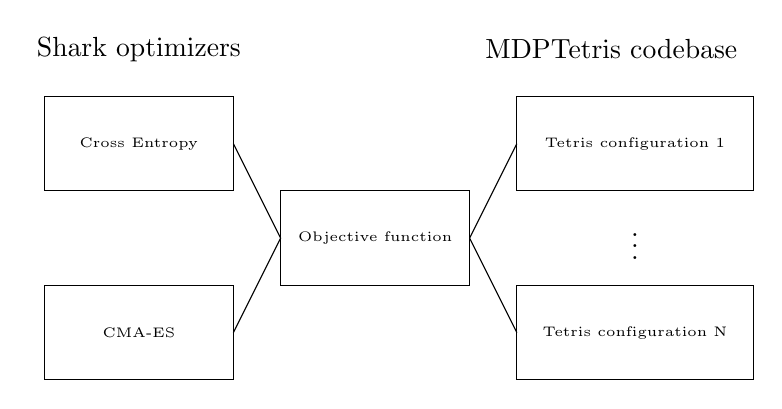
\begin{tikzpicture}[scale=0.6]
\draw  (0,0) rectangle (4,2);
\node at (2,1) {\tiny Objective function};
\draw  (-5,4) rectangle (-1,2);
\node at (-3,3) {\tiny Cross Entropy};
\draw  (-5,0) rectangle (-1,-2);
\node at (-3,-1) {\tiny CMA-ES};
\draw  (5,4) rectangle (10,2);
\draw  (5,0) rectangle (10,-2);
\node at (7.5,1) {$\vdots$};
\node at (7.5,3) {\tiny Tetris configuration 1};
\node at (7.5,-1) {\tiny Tetris configuration N};
\draw (-1,3) -- (0,1) -- (-1,-1);
\draw (5,3) -- (4,1) -- (5,-1);
\node at (-3,5) {Shark optimizers};
\node at (7,5) {MDPTetris codebase};
\end{tikzpicture}
\end{center}
\caption{Fusion of Shark and MDPTetris}
\end{figure}


The source code of the MDPTetris source code 
is accompanied with files that describe the
various existing features, that is files that defines 
the commonly used feature sets. As described, these files contains the identifiers of 
each feature to use, as well as two numbers respectively describing 
the agents reward function and how to evaluate a 'game over' state. 
The number for the reward function has remained unchanged at $0$ 
during all experiments. The "game-over" evaluation, for the
Bertsekas feature set, was initially set to $0$. Setting the 
"game-over" evaluation to $0$ means that the agent will not 
distinguish between regular moves and moves that results in losing
the game. If this setting remains at 0, the agent will always consult the
feature functions to rank its moves, yet setting this value to $-1$
the agent will always, regardless of feature functions, rank moves that ends
the game the lowest.
When running the experiments with this setting as $0$, a large portion
of the agents never exceeded a zero mean score. This occurs presumingly 
due to all agents failing quickly giving the optimization algorithm no 
useful feedback. However, setting the value
to $-1$, meaning that a "game-over" move yields $-\infty$ reward, 
none of the experiments got stuck on only zero scores. An example
of the layout of the feature file can be seen in figure \ref{fig:featfile}.
\begin{figure}[H]
\centering
\begin{lstlisting}
0    <- Describes the reward function
-1   <- Actions leading to game over is avoided at all cost
22   <- The policy contains 22 features
8 0  <- The feature with id 8 initially has weight 0
...  <- The remaining 21 features
\end{lstlisting}
\caption{Example of a file that describes a feature set. \label{fig:featfile}}
\end{figure}

\subsubsection{Game complexity \label{HardTetris}}
Both from other researchers and from the first experiments we executed, 
it quickly became clear that the time consumption of the optimization algorithms cannot be neglected.
Some papers suggests that running 10 executions of the Cross-entropy method
would take more than a month in total. These time estimates 
originates from experiments that were not conducted in parallel,
and on hardware from 2009, yet, the time consumption seemed to 
be a considerable issue.
In order to reduce the runtime of experiments 
to allow us more experiments in the evaluations, 
we can increase the "difficulty" of Tetris, by 
adjusting either the board size and/or adjusting the 
frequency of certain pieces. This has also been described 
before by Amine Boumaza, \citep{boumaza2009}.\\
To increase the difficulty of the game,
in our "Hard" Tetris, the s-block and z-block appear twice as often 
as the other pieces. As described by Boumaza, these pieces are the hardest to
place and will usually cause the player to produce holes and other irregularities
in the game board. Hence, the more frequent these pieces appear, the 
shorter the expected duration of the game.

\begin{figure}[H]
\begin{center}
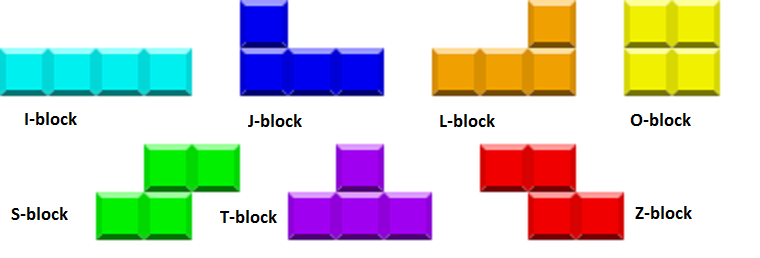
\includegraphics[scale=0.6]{img/Pieces}
\end{center}
\caption{Regular Tetris pieces \label{fig:TetrisPieces}}
\end{figure}

As using the harder version of Tetris, with the hard pieces appearing more frequent, shortens
the expected duration of a game and  the time it takes for an optimization algorithm 
to evaluate a search point, this configuration is indeed useful in searching for optimal parameters
of each algorithm. In the experiments leading to the best configurations of the two 
optimization algorithms, the harder version of Tetris is used. It is mentioned
by Amine Boumaza that using the harder to place pieces more frequently is a good method
for reducing the learning time, however, we have decided to conduct an experiment that explores
how the optimization algorithms behave when the game difficulty is changed.
We do expect that the learning curves develops much the same 
for both the hard and normal game difficulty, however
at lower scores for the harder setting.
To test if the difficulty setting has a significant impact, we used the Bertsekas
feature set (see table \ref{table:bertfeat}) and applied both the Cross-entropy 
Method and CMA-ES on the regular and hard configurations of Tetris.\\

\textbf{Results}\\
Table \ref{table:difficultyRes} renders the results of our experiments 
with with the hard and normal Tetris variants. CMA-ES and the Cross-entropy method 
were each applied 30 times to both game configurations. Table \ref{table:difficultyRes}
shows the means and quantiles of the scores gained in the last iteration.\\
The general settings of the experiments can be seen in the appendix section, \ref{AppendixGameComplexity}.

\begin{table}[H]
\centering
\small
\begin{tabular}{l l r r r r r}
Tetris Type & Optimizer & mean & Q1 & Q2 & Q3\\
\hline
Hard & Cross Entropy & $1633.607$ & $1357.170$ & $1606.565$ & $1938.71$\\
Normal & Cross Entropy & $100059.463$ & $79357.440$ & $105999.500$ & $111047.500$\\
Hard & CMA & $449.352$ & $201.850$ & $300.300$ & $529.350$\\
Normal & CMA & $49760.161$ & $42528.740$ & $49915.700$ & $67764.729$\\
\end{tabular}
\caption{Experiment testing game Normal Tetris against Hard Tetris \label{table:difficultyRes}}
\end{table}

\begin{figure}[H]
\centering
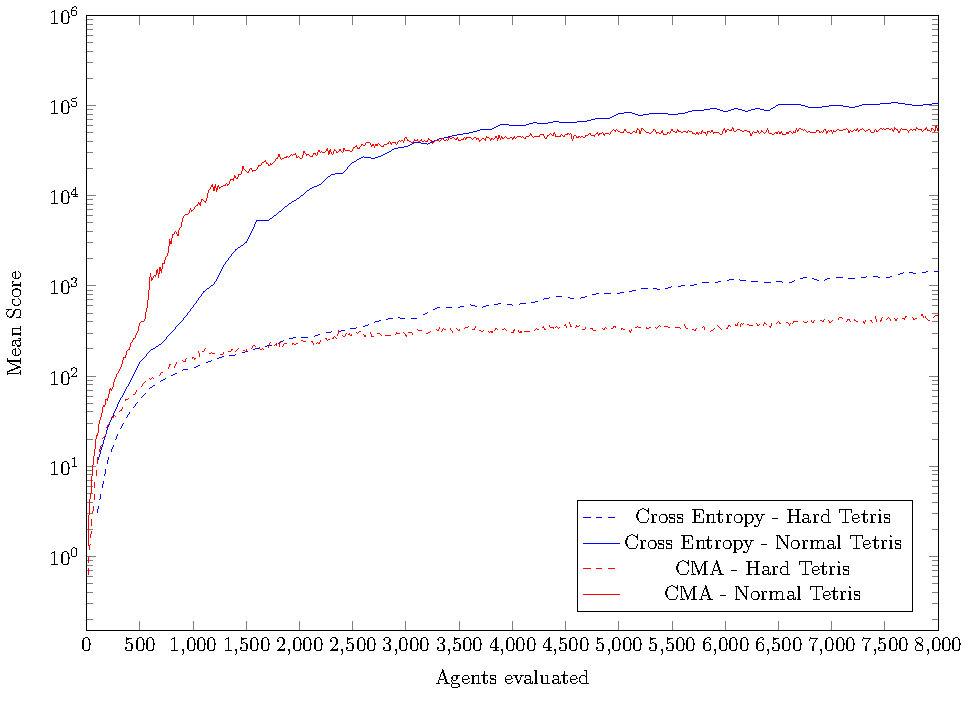
\includegraphics[scale=0.8]{data/complexity/mean/PlotFile.pdf}
\caption{Experiment testing Normal Tetris against Hard Tetris}
\end{figure}

\textbf{Analysis and discussion}\\
The results indicate that using Hard Tetris does not impact 
the general development of the algorithms, meaning we are 
able to use the harder Tetris for further experiments. 
From the graph it appears that the harder Tetris simply 
shifts the score compared to normal Tetris. However, we
will not use Hard Tetris for our final comparison experiments, to ensure that
the final conclusion is based on findings in the domain of the original problem. 
Therefore, we will primarily use Hard Tetris as a faster method for configuring
CMA-ES and the Cross-entropy method, especially when determining the optimal settings.
\\


\subsubsection{Comparison of feature sets  \label{compoffeatureset}}
As described in section \ref{prevWork}, there are different kind of feature sets which
impacts the performance of the agents. In our upcoming experiments, we are going to
use both the Dellacherie and Bertsekas feature set. For our initial comparison experiments
we are going to use the Bertsekas feature set, since other researchers report
a lower score with the Bertsekas feature set compared with the Dellacherie feature set
\citep{scherrer2009}. Compared to the \citep{scherrer2009} experiments, we don't want to maximize the
final score, but rather maximize the score with the lowest possible number of 
games evaluated.\\
It's important to note that we are not going to conduct comparison experiments with different
feature sets in the same experiment, since the algorithms needs to be on equal terms.\\
\\
We want to test whether the feature set has an impact on the performance of the algorithms,
therefore we want to test the two algorithms with both the Dellacherie and Bertsekas feature set.\\
\\
As the results from \ref{HardTetris} suggests, we consider usage of Hard Tetris \citep{boumaza2009} a valid means of asserting the performance difference in the algorithms with altering parameters.
Therefore, to prevent long runtimes, the following games were simulated
using Hard Tetris.\\

\textbf{Results}

In the following figures the mean results of 30 runs of both CMA-ES and the Cross-entropy method is presented. The settings for the Cross-entropy method remains at constant noise
with a noise term of $z^{(\generation)} = 4$ and an initial sigma of $\sigma_0 = 100$, 
and the CMA-ES with $\sigma_0 = 1$.\\
\\
Figure \ref{fig:featuresetCompareBertsekas} shows the experiment with the 
Bertsekas feature set. Which shows that when running the algorithms with a
harder game configuration, the algorithms behave mostly the same as with regular 
Tetris. Namely that CMA-ES converges faster than the Cross-entropy method, 
but is eventually outperformed.

\begin{figure}[H]
\begin{center}
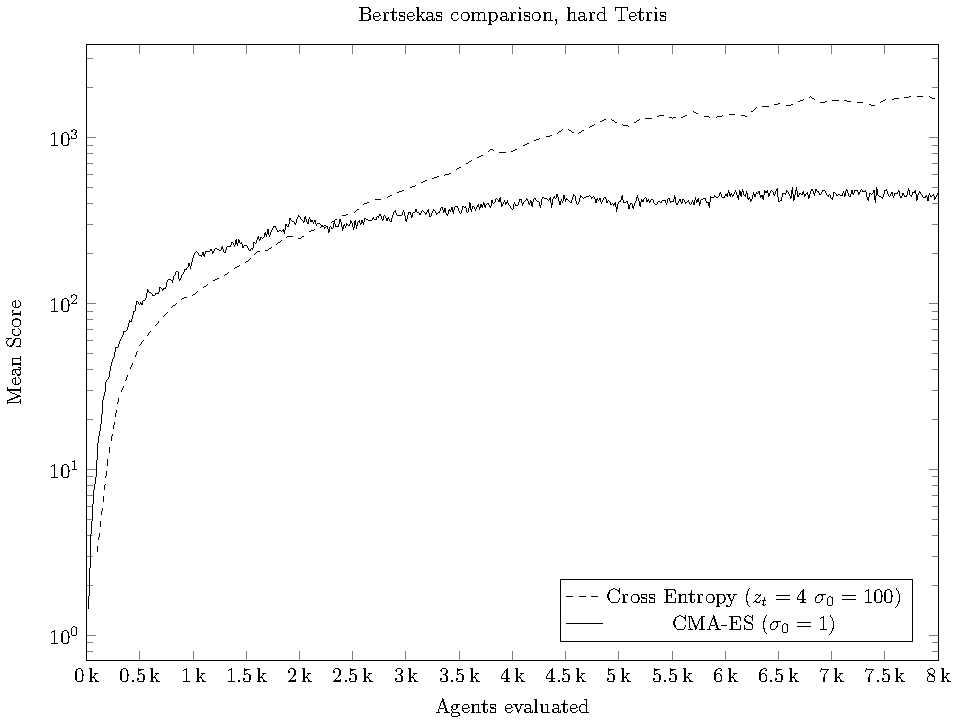
\includegraphics[scale=0.8]{plots/plotBertsekasCmaVsCEHardTetris}
\end{center}
\caption{Comparison between CMA-ES and the Cross-entropy method
using hard Tetris and the Bertsekas feature set 
\label{fig:featuresetCompareBertsekas}}
\end{figure}

When using the Dellacherie feature set a similar behaviour is observed.
However, the convergence seems to occur earlier and with a higher score
(figure \ref{fig:featuresetCompareDellacherie}).

\begin{figure}[H]
\begin{center}
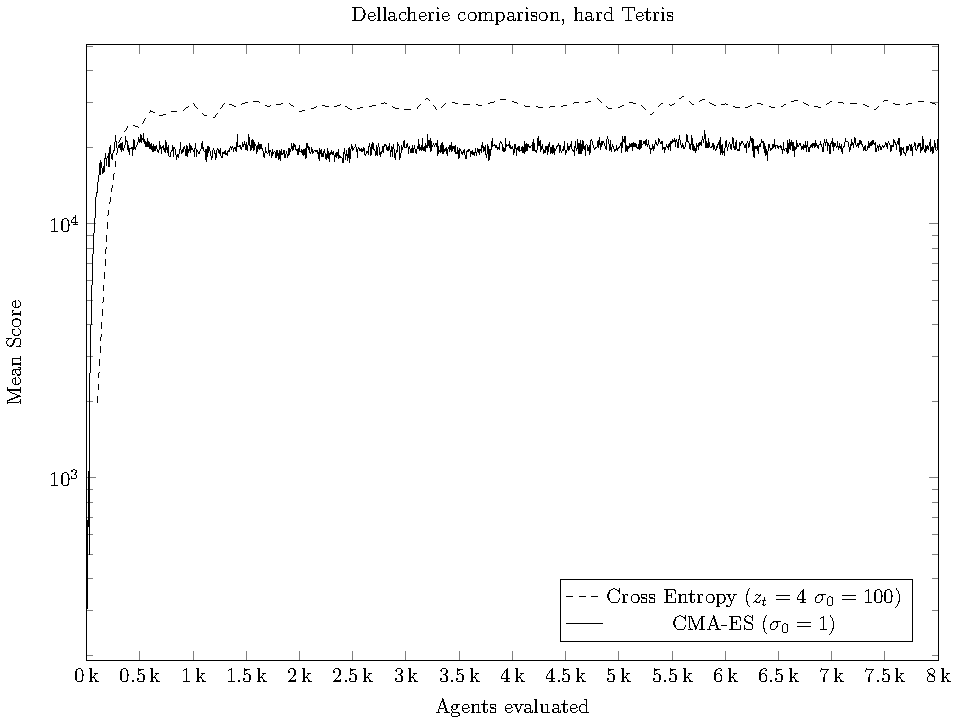
\includegraphics[scale=0.8]{plots/plotDellCmaVsCEHardTetris}
\end{center}
\caption{Comparison between CMA-ES and the Cross-entropy method 
using hard Tetris and the Dellacherie feature set
\label{fig:featuresetCompareDellacherie}}
\end{figure}

\textbf{Analysis and discussion}\\
The experiment with different feature sets indicates that the behaviour 
is not heavily dependant on the feature set.
It appears that changing the feature set simple shifts the score,
but does not affect the development of the graphs.\\
Therefore, we conclude that changing the feature set does not invalidate
the comparison of the two optimization algorithms. This means, that there's
no particular reason for using the Dellacherie feature set instead of the 
Bertsekas feature set, because neither CMA-ES or the Cross-entropy method seems
to benefit differently from the feature sets and the relative performance remains.


\subsection{Setup}

When executing the experiments, various parameters each have 
an impact on the final result of the learning curve. Thus, the parameters
are adjusted, first to match the experiments run by other researchers, 
and later to conduct as fair as possible comparisons between 
the Cross-entropy method and CMA-ES.\\
\\
% agents
The amount of vectors sampled in each generation $\populationSize$
has a high impact on the algorithm performance. By setting $\populationSize$
high, more policies are evaluated per iteration, and leads to a more thorough 
exploration of the search space. Thus the higher $\populationSize$ increases the
chances of finding a better mean for the next iteration.
However, higher $\populationSize$ also results in the
need for more evaluations per iteration. The goal for 
tuning this parameter is then
to set $\populationSize$ high enough to ensure 
exploration of good solutions, and yet 
low enough to avoid unnecessary evaluations.\\
In the implementation of CMA-ES from \shark , 
the algorithm  itself determines
the value of $\populationSize$ according to the 
size of the search space. 
The Cross-entropy method however, does not seem to have a 
general rule for this parameter,
so this value is manually adjusted to fit the 
problem as well as possible.\\
\\
% offspring
As both of the optimizing algorithm uses a subset of the sampled vectors
from a generation to update the distribution parameters, the number of 
offspring $\offspringNumber$ influences how the next generation is sampled.
By setting the value too high, the algorithm risks ceasing to progress any 
further since the updated mean would be too close to the previous one to 
significantly make a difference. By setting the value too low,
the risk of reaching a local optimum increases since the high-scoring agents
might have reached their high performance by chance.\\
The CMA-ES itself manages setting $\offspringNumber$ and the Cross-entropy method
is set according to the problem. Most authors that uses the Cross-entropy method for Tetris
sets the offspring size to $10\%$ of population size, that is 
$\offspringNumber = \lfloor 0.1 \cdot \populationSize \rfloor $.\\
\\
% Number of games per iteration
The number of games, $\numberOfEvaluations$, 
is the number of games  which each agent 
plays in each iteration. An agent's score is defined as the 
mean of the score of these 
$\numberOfEvaluations$ games.
We want this value low as possible, because as with the number of
agents, $\populationSize$, The number of games, $\numberOfEvaluations$, 
is another major factor in the run-time of the algorithm.
As Tetris is stochastic by nature, the score deviates a lot, 
even when the
same agent with the same policy plays multiple games. 
Hence, when assessing the true
performance of a policy it's rarely enough to play just few games. Thus, setting 
$\numberOfEvaluations$ high increases the likelihood of correctly choosing the best 
agents, yet, it also causes longer run times of the experiments.\\
\\
% Noise factor
Specific to the Cross-entropy method, 
most authors report that the performance of the 
algorithm increases dramatically when the sampling 
distribution is associated with
a noise term. The different types of 
noise are described in section \ref{CrossEntropy}.
The noise term is adjusted in order to 
prevent the algorithm from reaching a local optimum.
The current research shows that noise terms of $\noise^{(\generation)} = 4$ and 
$\noise^{(\generation)} = max \left( 5 - \generation / 10 \right)$ 
\citep{thiery:09} produces the best results.
The constant noise (such as $\noise^{(\generation)} = 4$) ensures that the algorithm
never settles in a too small area from which it samples, and forces it to explore
solutions that are further away from the mean. The further the 
algorithm progresses, 
the less noise is assumed needed, as the mean should approach a global optimum. to
address this, the linear decreasing noise 
is applied as it will lower the noise term
as the algorithm progresses.\\
\\
For the various experiments, these 
parameters will be tuned for the specific purpose 
at hand. In the verification of the Cross-entropy method, the parameters are set 
to match those reported in similar papers (\cite{thiery:09}, \cite{szita:06}).
In the comparison of the two algorithms, the parameters will be set such that 
the Cross-entropy method operates under as 
similar conditions as CMA-ES, to ensure an unbiased 
comparison.







\subsection{Verification of our implemented of the Cross-entropy method \label{varifyofce}}

Because the \shark\ library already contains an implementation of 
CMA-ES, but not an implementation of the Cross-entropy method, we extended the library
with our own implementation of the algorithm.\\
In order to verify the correctness of the implementation, 
we used the same experiments as used by 
Christophe Thiery and Bruno Scherrer \citep{thiery:09}. 
These experiments were used by Thiery and Scherrer to 
verify their own Cross-entropy method implementation with various types of noise correction. 
Therefore, we will perform the same experiments to verify our 
own contribution to the \shark\  library, by trying to achieve the same results.\\
\\
The setup is mirrored from the paper \citep{thiery:09}, 
with 100 agents ($\populationSize = 100$) per iteration,
and using the $\offspringNumber = 10$ best vectors
for the update step. After each iteration, 
an agent with the updated mean 
plays 30 games and the mean of these scores are recorded for the
learning curve.\\
During evaluation each agent plays one game, that is $\numberOfEvaluations = 1$.
A minor derivation from the figures present in \citep{thiery:09}, is 
the unit along the x-axis in the learning curve plots indicates 
the iteration number. As the experiments in this two algorithms
width variable population sizes are compared, the x-axis in all plots
indicated the number of Tetris games played during the learning. In one 
generation $\populationSize$ agents each play $\numberOfEvaluations$ games and hence
advance the x-axis by $\populationSize \numberOfEvaluations$.\\

\begin{figure}[H]
\begin{center}
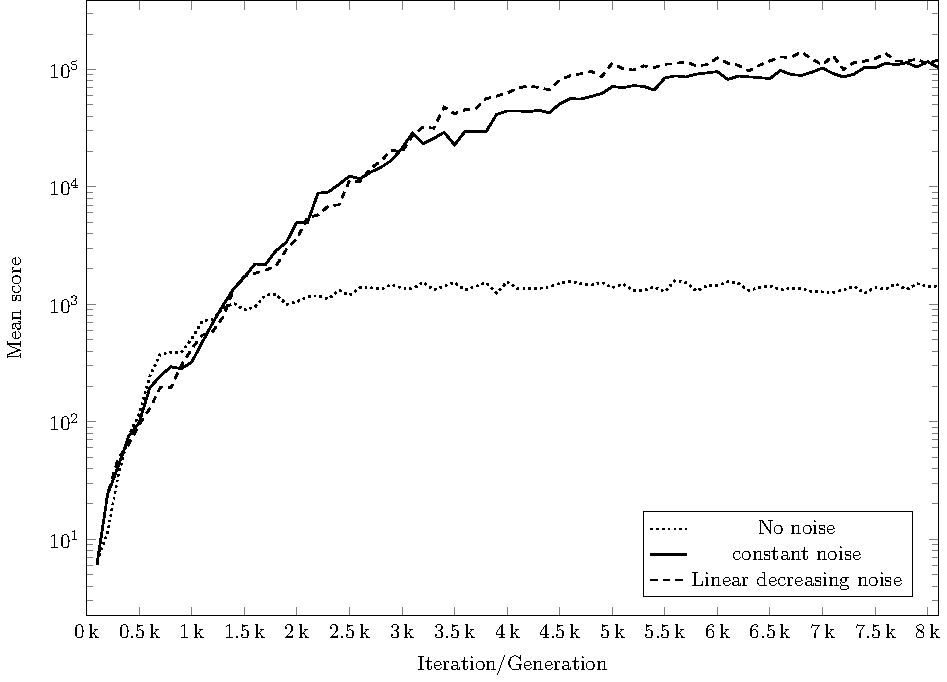
\includegraphics[scale=0.8]{plots/meansPlot}
\end{center}
\caption{Cross-Entropy mean performance \label{fig:cemean}}
\end{figure}

\clearpage
\begin{figure}[H]
\begin{center}
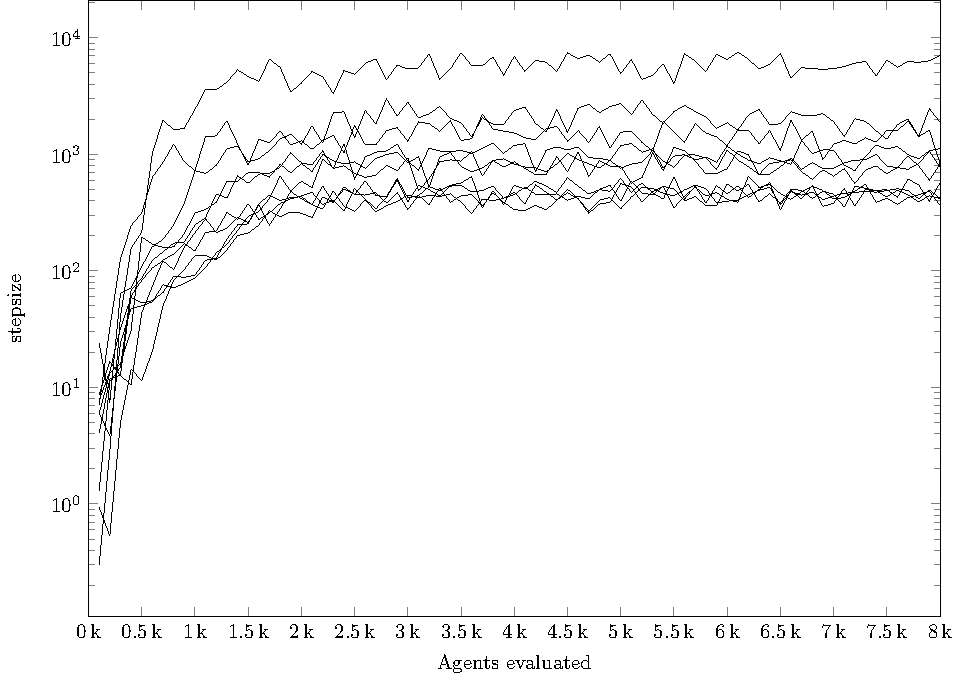
\includegraphics[scale=0.48]{plots/noNoisePlot}
\end{center}
\caption{No noise \label{fig:ceNoNoise}}
\end{figure}
\begin{figure}[H]
\begin{center}
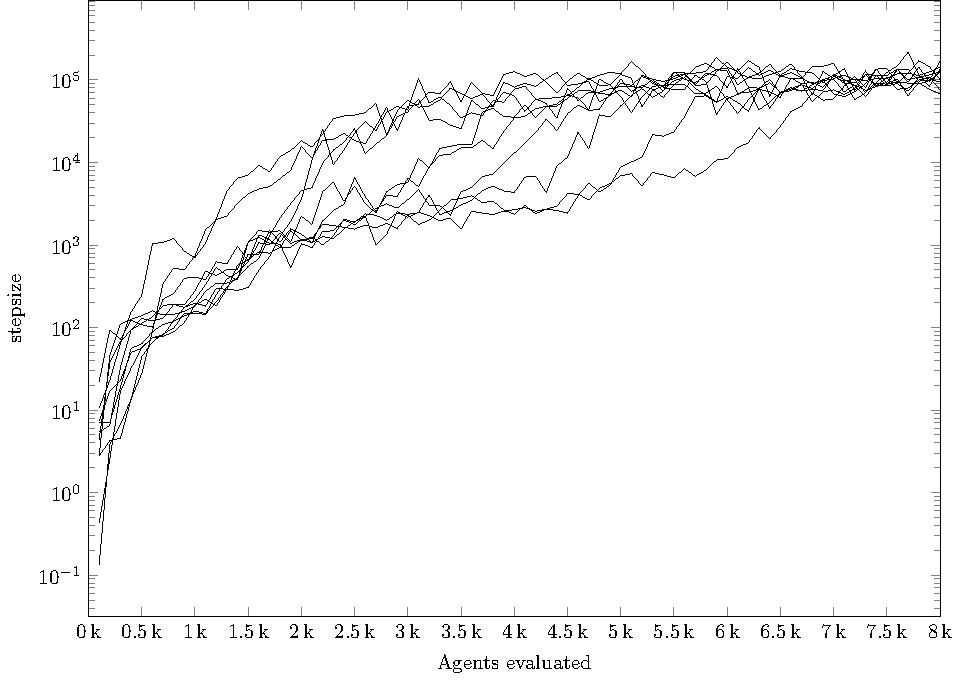
\includegraphics[scale=0.48]{plots/constantNoisePlot}
\end{center}
\caption{Constant noise \label{fig:ceCnstantNoise}}
\end{figure}
\begin{figure}[H]
\begin{center}
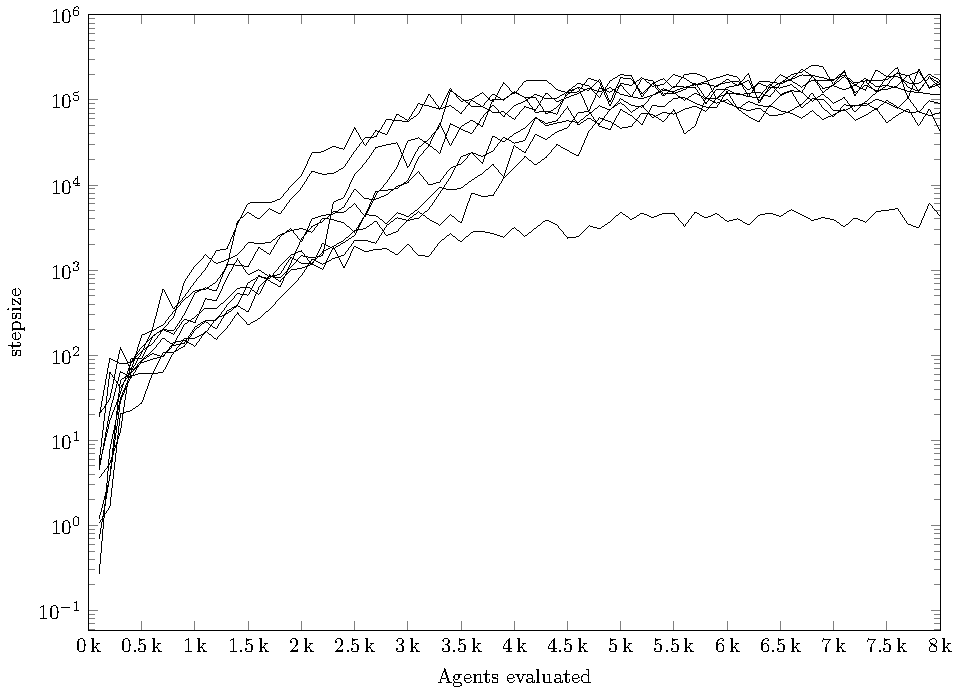
\includegraphics[scale=0.48]{plots/linearNoisePlot}
\end{center}
\caption{Linear decreasing noise \label{fig:ceLinNoise}}
\end{figure}

Figure \ref{fig:ceNoNoise}, \ref{fig:ceCnstantNoise} and
\ref{fig:ceLinNoise} shows 10 runs of each noise type. Figure
\ref{fig:cemean} shows the mean graph for each of the noise types.
The goal of these experiments were to replicate the experiments 
reported in \citep{thiery:09}. As the results seen from our experiments
to a high degree resemble those reported by Thiery et. al, we conclude
that our Cross-entropy method implementation works similar to theirs.\\
\\
When evaluating the score of the agent we also want to compute the confidence
interval in verifying the implementation of the Cross-entropy method. The mean agent plays 30 games
which leads to a confidence interval of $\pm36\%$ around the estimated mean,
which is similar to the confidence intervals in \citep{scherrer2009}.\\
By looking at the individual graphs for the different noise types 
(Figure \ref{fig:ceNoNoise}, \ref{fig:ceCnstantNoise} and
\ref{fig:ceLinNoise}), we get the following average scores.\\
\\
\textbf{Without noise (figure \ref{fig:ceNoNoise})}: The learning curve
stabilizes after 1,500 agents evaluated. And as it can be observed the
score variates much for the different executions between a score of 300 and 6,000
rows. This results in an average score of 1,400$\pm36\%$ rows.\\
\textbf{Constant noise (figure \ref{fig:ceCnstantNoise})}: 
The 10 executions reaches equivalent performances at some point, 
with a score between
54,000 and 154,000. This results in an average score of 105,000$\pm36\%$ rows.\\
\textbf{Linear decreasing noise (figure \ref{fig:ceLinNoise})}:
Most of the executions of this noise type settles around 200,000.
However, a single execution settled at a score of only around 5,000.
The mean performance of this noise type yielded a score of
120,000$\pm36\%$ \\

Based on the mean graphs and confidence interval compared to other papers, we can
hereby verify that our implementation of the Cross-entropy method works as intended. Even though the
experiments with linear decreasing noise in this case seems to outperform
the constant noise, other runs with linear decreasing noise ended in a mean 
performance of only 90,000$\pm36\%$. Yet, the constant noise is both from our
own experiments, and described in other research, noted to be the most reliable
noise type for reaching high scoring controllers \citep{scherrer2009}. 
Due to this, the constant noise is used in the 
benchmarking against CMA-ES.\\





\subsection{Optimal settings 
for the Cross-entropy method \label{optimalsettingsce}}

In this section we will determine the optimal settings for \begin{changebar}
\cbcolor{blue}
the Cross-entropy method
\end{changebar} through testing
of various adjustable parameters.\\
Compared to CMA-ES, the Cross-entropy method has fewer customizable parameters, more specifically 
only population-parent size and games played per agent.

\subsubsection{Population and selection size}
Other researchers run the Cross-entropy method with population size of
$\populationSize = 100$ and an offspring corresponding to 10\% of 
the population size, resulting in $\offspringNumber = 10$. As it's not 
discussed why this exact setting is applied, various settings of the Cross-entropy method
was executed to asses the performance of other configurations
in our experiments.
The experiments includes different population sizes 
$\populationSize \in \{12, 22, 50, 100, 200\}$ and offspring 
sizes of either $10\%$ and $50\%$ (since the CMA-ES algorithm by default
uses $50 \%$ selected vectors). 
A summary of the experiments can be seen in figure \ref{CEConfigTest}
on page \pageref{CEConfigTest}.

\begin{figure}[H]
\centering
\begin{tabular}{r r | r r r r}
$\populationSize$ & $\offspringNumber$ & mean & Q1 & Q2 & Q3\\
\hline
13 & $10\%$  & 1585,3     & 93,0      & 113,5        & 220,7\\
13 & $25\%$  & 30.496,9   & 15.222,1  & 20.264,2     & 39.019,8\\
13 & $50\%$  & 39.824,2   & 26.457,0  & 33.663,4     & 49.743,7\\
22 & $10\%$  & 35.841,6   & 20.391,9  & 42.045,5     & 48.464,6\\
22 & $25\%$  & 80.884,9   & 56.042,5  & 71.900,2     & 78.653,4\\
22 & $50\%$  & 52.887,4   & 23.531,9  & 42.161,0     & 83.144,1\\
50 & $10\%$  & 95,623,1   & 82.738,9  & 93.388,9     & 111.351,5\\
50 & $25\%$  & 110.525,0  & 103.128,1 & 111.195,5    & 121.974,4\\
50 & $50\%$  & 69.130,7   & 52.511,0  & 64.351,6     & 91.488,6\\
\hdashline
100 & $10\%$ & 115.868,7  & 84.368,5  & 122.238,5    & 146.457,0\\
\hdashline
100 & $25\%$ & 70.011,1   & 58.008,0  & 69.588,2     & 80.432,7\\
100 & $50\%$ & 22.910,4   & 4.037,7   & 14.353,7     & 47.215,9\\
200 & $10\%$ & 85.181,7   & 45.201,5  & 96.803,1     & 117.578,0\\
200 & $25\%$ & 32.894,6   & 8688,7    & 25.333,1     & 58.434,8\\
200 & $50\%$ & 946,4      & 585,0     & 802,5        & 1.267,7
\end{tabular}
\caption{the Cross-entropy method configuration test, 
see Appendix \ref{appendixCrossEntropyConfig} for the full plots 
of the experiments.  \label{CEConfigTest}}
\end{figure}

The experiments with different population and parent sizes
does not seem to support a choice for any other configuration 
than the mostly commonly used 
$\populationSize = 100$ and $\offspringNumber = 10$. \\
However, with a configuration of $\populationSize = 50$ and $\offspringNumber = 12$ convergence
is achieved faster (see figure \ref{fig:bestConfCE}). This means that the score limit is reached faster, which
results in longer computation time, than the $\populationSize = 100$ and $\offspringNumber = 10$
configuration. In other words, the $\populationSize = 100$ and $\offspringNumber = 10$ configuration 
is therefore preferred since it takes shorter computation time and the end-result is similar compared
to the $\populationSize = 50$ and $\offspringNumber = 12$ configuration, even though the latter 
configuration from our expriments converged faster. The experiments also apppears
to suffer from a high noise, yet both the mean and the quantiles favor the 
extensively tested the Cross-entropy method configuration of $\populationSize = 100$ and $\offspringNumber = 10$.

\begin{changebar}
\cbcolor{blue}
\begin{figure}[H]
\begin{tabular}{@{}l@{}l@{}}
\includegraphics[scale=1]{plots/ce_ConstantNoise_l50_o12_all} &
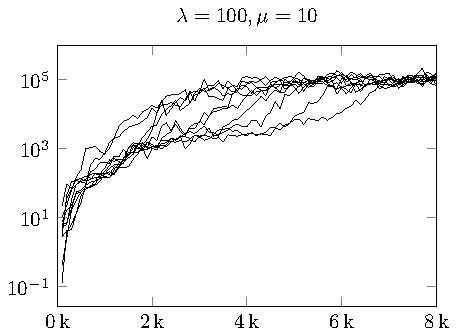
\includegraphics[scale=1]{plots/ce_ConstantNoise_l100_o10_all}
\end{tabular}
\caption{The two best configurations of the Cross-entropy method 
\label{fig:bestConfCE}}
\end{figure}
\end{changebar}

\subsubsection{Games per agent \label{GamesPerAgentCESection}}
Another parameter we can adjust is the number of 
games played each agent plays per generation. By playing
multiple games with each agent and using their 
mean score to compute the next generation mean. This
secures a higher chance of a better offspring generation,
but at the cost of more games
evaluated.\\
Table \ref{GamesPerAgentCE} shows the different values of
games per agent we are going to be
testing.

\begin{table}[H]
\centering
\begin{tabular}{c c c}
Population Size & Parent size & Games per Agent\\
\hline
$13$ & $10\%$ & 1/3/5/7/10\\
$13$ & $25\%$ & 1/3/5/7/10\\
$13$ & $50\%$ & 1/3/5/7/10\\
$22$ & $10\%$ & 1/3/5/7/10\\
$22$ & $25\%$ & 1/3/5/7/10\\
$22$ & $50\%$ & 1/3/5/7/10\\
$50$ & $10\%$ & 1/3/5/7/10\\
$50$ & $25\%$ & 1/3/5/7/10\\
$50$ & $50\%$ & 1/3/5/7/10\\
$100$ & $10\%$  & 1/3/5/7/10\\
$100$ & $25\%$  & 1/3/5/7/10\\
$100$ & $50\%$ & 1/3/5/7/10\\
$200$ & $10\%$ & 1/3/5/7/10\\
$200$ & $25\%$ & 1/3/5/7/10\\
$200$ & $50\%$ & 1/3/5/7/10
\end{tabular}
\caption{Games per agent of the Cross-entropy method experiment setup\label{GamesPerAgentCE}}
\end{table}

The experiments includes different games per agent of $\{1,3,5,7,10\}$. By increasing the number of games 
played per agent, we are increasing the evaluation cost by a multiplication factor in exchange for a more 
accurate evaluation of each agent. This is to avoid misconceiving poor performing agents
for good ones, as multiple evaluations will decrease the chance the agent having 
'lucky games'. However, we wish to find 
the best performing configuration with the lowest cost and maximum benefit, and evaluating multiple 
times will increase the function cost.\\
\\
\textbf{Results}\\
The total number of configuration experiments is 75, with 30 individual experiments each,
resulting in a total of
\begin{changebar} 
2,250
\end{changebar} 
individual experiment runs. These results are all included in 
appendix \ref{appendixCEPopulationParent}.\\
Below in table \ref{CEBestConfigTable} and figure \ref{CEBestConfigPlot}, the five best
best resulting configurations are depicted. We chose these by first selecting the best 
configuration of each Population-Parent size. This resulted in three
configurations for each Population-Parent size, which we then compared to determine the best
configuration for each Population-Parent size. Which is depicted in table \ref{CEBestConfigTable} and figure \ref{CEBestConfigPlot}.
\begin{table}[H]
\centering
\small
\begin{tabular}{r r r r r r r}
Population & Parent & Games per Agent & mean & Q1 & Q2 & Q3\\
\hline
$12$ & $6$ & 10 & $2109.837$ & $1802.968$ & $2021.165$ & $2276.652$\\
$22$ & $5$ & 5 & $2371.793$ & $2013.168$ & $2412.815$ & $2708.931$\\
$50$ & $12$ & 5 & $2749.991$ & $2605.171$ & $2702.400$ & $2835.960$\\
$100$ & $25$ & 3 & $2776.560$ & $2397.691$ & $2742.950$ & $3027.541$\\
$200$ & $50$ & 1 & $2950.767$ & $2564.118$ & $2841.065$ & $3377.189$\\
\end{tabular}
\caption{Best configurations of all population sizes - the Cross-entropy method \label{CEBestConfigTable}}
\end{table}

\begin{figure}[H]
\centering
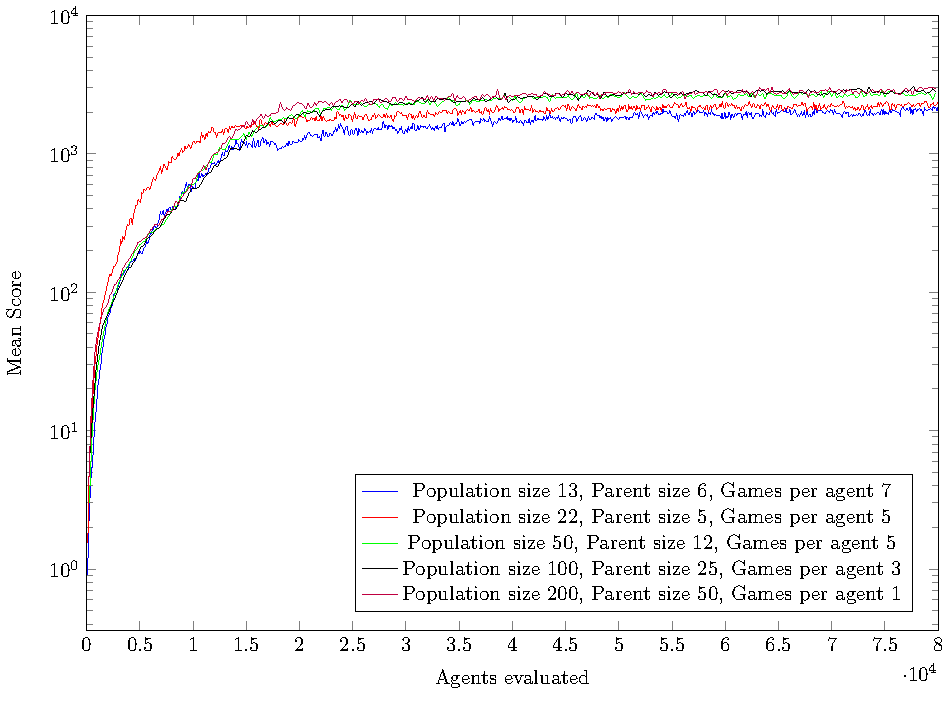
\includegraphics[scale=0.8]{data/ce_population_offspring/bestofall_population/PlotFile.pdf}
\caption{Best configurations of all population sizes - the Cross-entropy method \label{CEBestConfigPlot}}
\end{figure}

From table \ref{CEBestConfigTable} and figure \ref{CEBestConfigPlot}, we can see that population size 50 with parent size 12 and 5 games per agent, population size 100 with parent size 25 and 3 games per agent, and, population size 200 with parent size 50 and 1 game per agent, performs almost identically.\\

\textbf{Discussion and analysis}\\
From the graph and the table depicting the quantiles, it appears that the configuration
population size 200 with parent size 50 and 1 game per agent yields the best performance. 
It achieves the highest score with the fastest convergence of all the candidate solutions
we have listed.\\
Therefore, we will be using this configuration for the tuned comparison experiments.


\subsection{Optimal settings 
for CMA \label{optimalsettingscma}}

When finding the optimal settings for CMA we have a larger set of parameters we can adjust compared
to Cross Entropy. Again, as the same with Cross Entropy, we can adjust the population/parent size and
games per agent. Furthermore we can adjust the initial step-size, lower bound and recombination type.\\
The following sections will go into detail how these parameters affect the performance of CMA
algorithm. In the last section we will perform experiments to determine the optimal settings.

%In previous sections we focused on tuning Cross Entropy for the Tetris 
%problem. Whereas we deliberately chose not to tune CMA due to its implementation 
%into the Shark library \citep{shark08}. However, experiments with the "out of 
%the box" CMA from Shark, with default settings vs the tuned Cross Entropy
%resulted in CMA reaching convergence very fast but not achieving the same point
%limit as Cross Entropy.\\

\subsubsection{Recombination type}
Furthermore, CMA also has a unique formula for calculating the updated mean,
called the 'Recombination type' \ref{CMAtheory}. Where the recombination type
determines how much influence each of the offspring vectors has on the next
generation. Built into the CMA algorithm is three methods of recombination. 
\begin{itemize}
\item EQUAL, Each of the offspring vectors has equal influence in the generated mean.
\item LINEAR, The best of the offspring vectors has more influence. 
\item SUPERLINEAR, The vectors are weighted with a logarithmic equation.
\end{itemize}
\begin{changebar}
As default, CMA uses Super Linear recombination. However, Tetris is a problem
with multiple local optimums and heavy noise in its search space. 
\end{changebar}
This means, though a vector may be the best in its generation,
it could be a nearby local optimum. Therefore,
Super Linear recombination may not be the optimal recombination type for the Tetris problem.\\

The recombination types are covered in section \ref{CMAtheory} on 
page \pageref{eq:recomType}.


\subsubsection{Population and selection size}
By adjusting the population size to that similar of Cross Entropy, we are able
to get a fair comparison between the two algorithms, given each generation will
contain the same number of agents. By setting the population and parent size
to the same values, we in effect test if the covariance matrix and the step-size
control has a impact on the algorithm performance compared to Cross Entropy
which does not have the features.\\
Table \ref{CMAPopulationSelectionConfigTest} displays the values that we are going
to test for the population and selection size.

\begin{changebar}
\cbcolor{blue}
\begin{table}[h]
\centering
\begin{tabular}{r r}
Population size, $\populationSize$ & Parent size, $\offspringNumber$\\
\hline
$12$ & $1$\\
$12$ & $3$\\
$12$ & $6$\\
$22$ & $2$\\
$22$ & $5$\\
$22$ & $11$\\
$50$ & $5$\\
$50$ & $12$\\
$50$ & $25$\\
$100$ & $10$\\
$100$ & $25$\\
$100$ & $50$
\end{tabular}
\caption{CMA-ES configuration for population and parent size \label{CMAPopulationSelectionConfigTest}}
\end{table}
\end{changebar}

The experiments includes different population $N \in \{12,22,50,100\}$ and offspring sizes of either
10\%, 25\% and 50\%. We use 10\% because of the Cross Entropy recommended selection size, while
we use 25\% because of CMA-ES's standard selection size for the EQUAL recombination type. 
Furthermore we use 50\% because of CMA-ES's standard selection size for the LINEAR and SUPERLINEAR 
recombination type.

\subsubsection{Games per agent \label{CMAGamesPerAgentSection}}
As with Cross Entropy we can also adjust the number of games each agent plays per generation.
However, because of the recombination type for CMA, one game pr. agent may  be insufficient to assess the
performance of an agent. The Linear and Super Liner recombination types will value the better agents higher.
Therefore, it may occur that some better-on-average agent encounter an unlucky game, achieving a lower score than
it's actual potential allows. \\
Thus, evaluating each agent multiple times and using the average score for recombination may allow for a more accurate assessment.\\

The experiments includes different games per agent of $\{1,3,5,7,10\}$. We have chosen the same 
values as with Cross Entropy to get comparable results (see section \ref{GamesPerAgentCESection}).

\subsubsection{Initial step-size \label{sec:CMAInitialStepSize}}
Initially, the covariance matrix of CMA in generation $\generation = 0$
is the identity matrix. The initial step-size, $\sigma_0$, will hence in 
the first iteration scale the area in which the CMA algorithm searches.
As from section \ref{normalSamples}, it's known that the scale of the 
solutions has no impact on the scores. Hence, it's assumed that the initial 
step-size should not have any major impact on the results.

\begin{figure}[H]
\centering
\begin{tabular}{r | r r r r r}
$\sigma_0$ & mean & Q1 & Q2 & Q3\\
\hline
0.1 & 50769.3 & 21301.1 & 54588.7 & 73972.4\\
0.2 & 42290.6 & 32180.2 & 42290.6 & 49337.4\\
0.5 & 53893.7 & 14211.1 & 66773.0 & 85816.7\\
0.8 & 37557.7 & 1422.8  & 15450.8 & 93719.4\\
1.0 & 49537.9 & 31369.8 & 49537.4 & 58454.6
\end{tabular}
\caption{Results of CMA-ES with adjusted initial step-size \label{CMAInitialSigmaConfigTest}}
\end{figure}
The full graphs of the results from this experiment can be seen in 
appendix \ref{appendixCMAInitialSigma}.\\
For the initial experiments using CMA-ES, 
the only adjusted parameter is the initial 
step-size $\sigma_0$. The configurations of step-sizes were 
$\sigma_0 \in \{0.1, 0.2, 0.5, 0.8, 1.0\}$. As the table shows,
the final mean score does not seem to change with the initial step-size.
Furthermore, the adjustment of the step-sizes does not appear to 
have a drastic impact on the mean scores. However, based on both mean score and
quantiles, the best configuration seems to be $\sigma_0 = 0.5$. This is 
is also referred to as a typical initial setting in \citep{boumaza2009}.
Therefore, the conclusion remains that the initial step-size is not critical 
for the experiment.\\

To tell if the step-size is actually a significant parameter to adjust, results from 
the two best performing configurations are compared using the Mann-Whitney-Wilcoxon test\footnote{\url{https://stat.ethz.ch/R-manual/R-patched/library/stats/html/wilcox.test.html}}.
The Mann-Whitney-Wilcoxon test has the appealing property that it does not require any parameters
besides the actual data to test, and it does not require the assumption that data originates 
from a Gaussian distribution. The test accepts data from two populations, that may or may not 
be drawn from the same underlying distribution and will test against the null hypothesis, 
namely that the two populations have identical distribution. If the test concludes a 
confidence less then $5\%$ ($p < 0.05$), we cannot firmly reject the null hypothesis, 
and cannot conclude any significant difference in the population. From the experiments
with the initial sigma setting, the immediate choice of $\sigma_0$ would be 0.5.
The Wilcoxon test is applied to the data from the runs with $\sigma_0 \in \{0.5, 1\}$
using R\footnote{\url{https://cran.r-project.org/}}. The data supplied
to the wilcoxon test consists of the the mean scores from the last generation.
This test gives $p=0.5619$, which means that we cannot reject that the two 
populations differ, and the initial sigma is considered not to play a significant 
for the CMA-ES applied to Tetris.

\subsubsection{Lower bound}

As with the Cross Entropy method, to avoid early convergence
at a too low local optimum, a 
certain lower threshold for the variance should be applied when 
sampling vectors for solutions. In the Cross Entropy method, a constant 
noise term $z^{(\generation)} = 4$ i added to the variance for each component
of the sampled vectors. When the $i$'th component in cross entropy is
sampled as follows
\begin{align*}
\individual_i &\sim \mathcal{N}\left(m, \sigma^{2}\right)\\
              &\sim \sigma \mathcal{N}\left(m, 1\right)
\end{align*}
Then $\sigma^{2} \geq 4$. To gain the same effect for the CMA, a lower bound 
is applied to the step-size. Such a bound is implemented in the Shark library
as the following, where the value of the lower bound is $l$.
\begin{align*}
\sigma  \lambda_n \geq l
\end{align*}
Where $\lambda_n$ is the lowest eigenvalue in the covariance matrix. 
When the vectors are sampled, the samples are scaled by the matrix $D$
containing the eignvalues of the covariance matrix. 
Hence, if $\sigma \lambda_n \geq l$, then the smallest scaling
that takes place is at least $l$. As the vectors can be written 
as
\begin{align*}
\individual &\sim \mean + \sigma B 
\underbrace{D \mathcal{N}\left(0, I \right)}_{\mathcal{N}\left(0, D^2 \right)}
\end{align*}
Where $D \mathcal{N}\left(0, I \right)$ corresponds to 
$\mathcal{N}\left(0, D^2 \right)$ which, since $D$ is a diagonal
matrix, is just the same type of sampling as in Cross Entropy. 
The matrix $B$ will only rotate the the sampled vectors, and finally,
$\sigma$ will perform an isotropic scaling. 
To roughly resemble the constant noise configuration of Cross Entropy,
when sampling vectors, the lowest variance may not drop below 4. 
This is achieved by setting a lower bound $l=2$. If this applies,
the sampling can be written as
\begin{align*}
\individual &\sim \mean +  B \mathcal{N}\left(0, \sigma^2 D^2 \right)
\end{align*}
Where, with $l=2$, the lowest entry in the diagonal matrix $\sigma^2 D^2$
is $4$.\\
\\
To see if this setting makes sense, the CMA-ES was run with lower bounds as 
$l \in \{0.5, 2.0, 4.0\}$ with the results shown in figure \ref{CMALowerBoundConfigTest}.

\begin{figure}[H]
\centering
\begin{tabular}{r | r r r r r}
$l$ & mean & Q1 & Q2 & Q3\\
\hline
0.5 & 42800.7 & 6780.8  & 36863.0 & 74722.5\\
2.0 & 80733.4 & 62357.4 & 84349.0 & 108007.5\\
4.0 & 61497.2 & 55621.7 & 64940.1 & 81991.6\\
\end{tabular}
\caption{Results of CMA-ES lower bounds \label{CMALowerBoundConfigTest}}
\end{figure}
The raw graphs for this experiment is present in appendix \ref{appendixCMALowerBound}.\\
Evidently, the setting of a lower bound $l=2.0$ appears as the preferable choice, and this 
setting adopted across all further experiments.


\subsubsection{Experiment for finding the optimal settings \label{OptimalSettingsCMA}}
In this in section we are going to conduct a wide variety of experiments to determine
the best settings for CMA. More specifically we are going to find the best combination for
population size, parent size and games per agent.\\
Table \ref{SuperCMAExperiment} depict the different experiments we are
going to carry out.

\begin{table}[H]
\centering
\begin{tabular}{c c l c}
Population Size & Parent size & Recombination Type & Games per Agent\\
\hline
$12$ & $1$ & EQUAL/LINEAR/SUPERLINEAR & 1/3/5/7/10\\
$12$ & $3$ & EQUAL & 1/3/5/7/10\\
$12$ & $6$ & LINEAR/SUPERLINEAR & 1/3/5/7/10\\
$22$ & $2$ & EQUAL/LINEAR/SUPERLINEAR & 1/3/5/7/10\\
$22$ & $5$ & EQUAL & 1/3/5/7/10\\
$22$ & $11$ & LINEAR/SUPERLINEAR & 1/3/5/7/10\\
$50$ & $5$ & EQUAL/LINEAR/SUPERLINEAR & 1/3/5/7/10\\
$50$ & $12$ & EQUAL & 1/3/5/7/10\\
$50$ & $25$ & LINEAR/SUPERLINEAR & 1/3/5/7/10\\
$100$ & $10$ & EQUAL/LINEAR/SUPERLINEAR & 1/3/5/7/10\\
$100$ & $25$ & EQUAL & 1/3/5/7/10\\
$100$ & $50$ & LINEAR/SUPERLINEAR & 1/3/5/7/10
\end{tabular}
\caption{Full experiments overview \label{SuperCMAExperiment}}
\end{table}

The choice behind using the above population sizes is to use the same population sizes as
when we tuned Cross Entropy (see section \ref{optimalsettingsce}). However, we use a population
size of 12 instead of 10, because a population size of 12 is the stock setting for Shark CMA \citep{shark08}.\\
In regards to the parent size, they have been determined depending on the recombination type.
We use all three different recombination types for the 10\% parent sizes to make these experiments
correspond to the Cross Entropy settings (see section \ref{optimalsettingsce}). However, Shark CMA
has predetermined parent sizes for each recombination types, 25\% for EQUAL and 50\% for both
LINEAR and SUPERLINEAR \citep{shark08}. For this reason we also conduct experiments for each population
size to represent these Shark CMA preferred settings.
Furthermore we also test different number of games per agent as for the reason presented in section \ref{CMAGamesPerAgentSection}.\\\\
These experiments will be conducted using Hard Tetris (see section \ref{HardTetris}), in order
to lower the computation time.\\

\textbf{Results}\\
The total number of configuration experiments is 120, with 30 individual experiments each,
resulting in a total of 3.600 individual experiment runs. These results are all included in 
appendix \ref{appendixCMAPopulationParent}.\\
Below in table \ref{CMABestConfigTable} and figure \ref{CMABestConfigPlot}, the four best
best resulting configurations are depicted. We chose these by first selecting the best 
configuration of each Population-Parent size with each recombination type. This results in six
configurations for each Population-Parent size, which we then compare to determine the best
configuration for each Population-Parent size, regardless of recombination type. Which is depicted in table \ref{CMABestConfigTable} and figure \ref{CMABestConfigPlot}.

\begin{table}[H]
\centering
\small
\begin{tabular}{c c l c r r r r}
Population & Parent & Recombination & Games per Agent & Mean & Q1 & Q2 & Q3\\
\hline
$12$ & $6$  & SUPERLINEAR & 10 & $2472.293$ & $2194.049$ & $2430.780$ & $2709.040$\\
$22$ & $11$ & SUPERLINEAR & 10 & $2849.220$ & $2500.231$ & $2835.450$ & $3143.121$\\
$50$ & $25$ & SUPERLINEAR & 5  & $3211.658$ & $2889.689$ & $3305.485$ & $3694.480$\\
$100$ & $50$ & LINEAR     & 7  & $3322.076$ & $3160.098$ & $3289.370$ & $3537.850$
\end{tabular}
\caption{Best performing configurations of all population sizes \label{CMABestConfigTable}}
\end{table}

\begin{figure}[H]
\centering
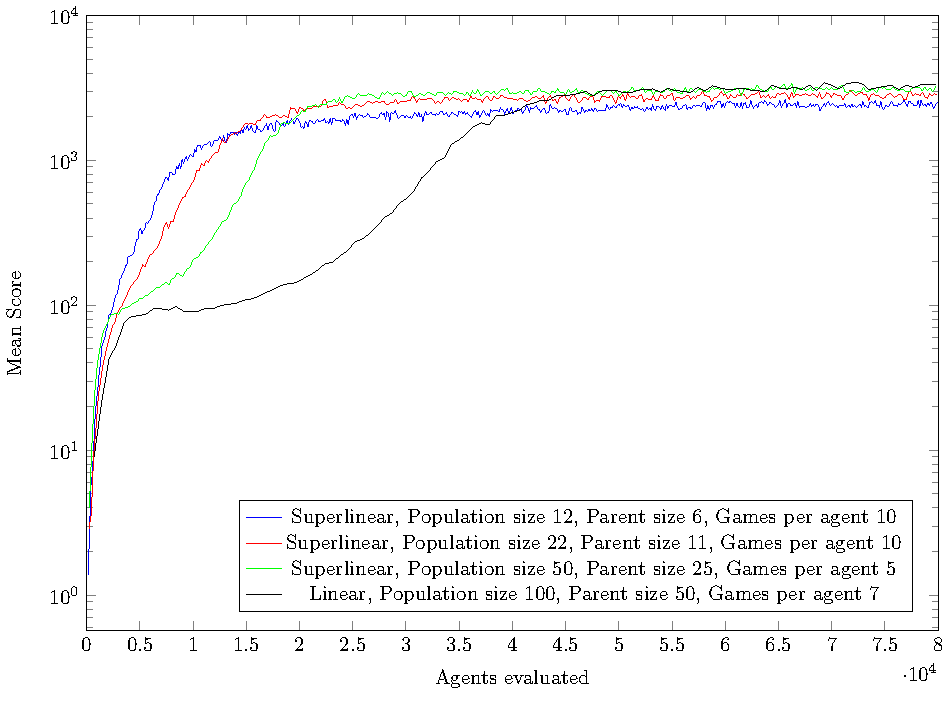
\includegraphics[scale=0.8]{data/cma_population_offspring/bestofall_population/PlotFile.pdf}
\caption{Best performing configurations of all population sizes \label{CMABestConfigPlot}}
\end{figure}

From table \ref{CMABestConfigTable} and figure \ref{CMABestConfigPlot}, we can see that
Linear recombination type, with population size 100, parent size 50 and 7 games per agent
(black) yields a better score compared to Superlinear with population size 50, parent size 25 and 5 games per agent (green).
However, green has a much faster convergence than black and almost reaches the same score.\\

\textbf{Analysis and discussion}\\
Because the green converges almost twice as fast as black, but reaches practically the same
score, we opt to use the Superlinear with population size 50, parent size 25 and 5 games per agent for the comparison experiments.\\
Therefore, we will be using this configuration for the tuned comparison experiments.











\subsection{Comparison between the Cross Entropy and CMA-ES}

In this section, we present the actual comparison experiments between the Cross-entropy method
and CMA-ES.
In the first experiment, we conduct a comparison experiment using the 
"default" settings for both CMA-ES and the Cross-entropy method. We use this experiment to
get an initial idea of how the two algorithms compare to each other, when using the commonly
used algorithm parameters.
In the second experiment, we conduct an experiment using the "optimized" settings
specified in section \ref{optimalsettingsce} for the Cross-entropy method and section
\ref{optimalsettingscma} for CMA-ES.\\
These experiments are used to conclude whether CMA-ES or the Cross-entropy method
is the better algorithm for learning Tetris.


\subsubsection{Initial comparison}
For the initial comparison we use the Bertsekas featureset, since the same featureset
was used for verifying the Cross Entropy implementation. Furthermore, others researchers
has used the Bertsekas featureset as a benchmarking standpoint \citep{thiery:09} \&
\citep{szita:06}.\\
The goal of this comparison is to get an initial idea of how the Shark implementation of
CMA compares to Cross Entropy.\\

\textbf{Results}

Using Cross Entropy with the constant noise setting and CMA with an initial step-size
of $0.5$, we get the following results, seen in figure \ref{fig:CMA_VS_CE_00}.\\

\begin{figure}[H]
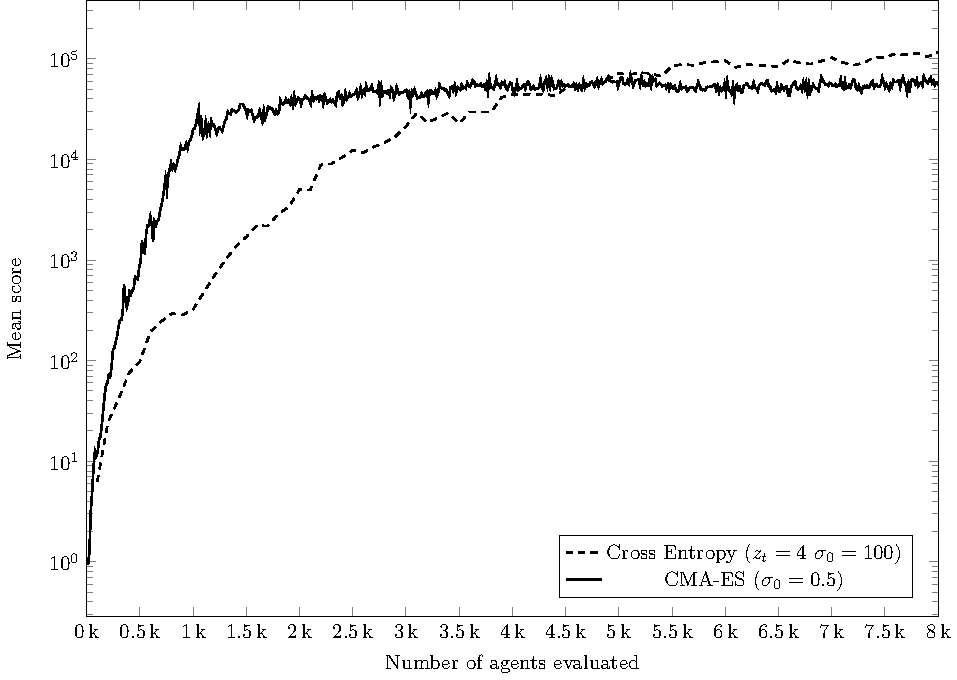
\includegraphics[scale=1]{plots/cmaCePlot}
\caption{Initial comparison between CMA-ES and Cross Entropy \label{fig:CMA_VS_CE_00}}
\end{figure}

As figure \ref{fig:CMA_VS_CE_00} reveals that CMA converges faster,
but reaches a local optimum at around 2,000 games played. Meanwhile CE has a 
slower convergence but reaches a better mean score compared to CM at around 5,500
agents evaluated. In detail, CMA on average reaches a score of 50,000 rows, and
CE reaches a score of 100,000.\\

\comment{Add the raw graphs to appendix}

\textbf{Analysis and discussion}

These results clearly defy our initial hypothesis as we predicted
for CMA to outperform CE, due to its more sophisticated nature. 
One reason for this outcome could possibly be that
CMA has a very little population size compared to Cross Entropy,
which could be a decisive lack as the objective function is noisy with 
a high variance. These results indicate a need to adjust the CMA
configuration, to prevent the too fast convergance.

Among the possible adjustments are:\\
\\
\textit{Enlargment of population size}\\
As the population size is quite small (only around 13)
for this experiment, the CMA algorithm might not be able
extract enough information at each generation. As seen in 
section \ref{optimalsettingsce}, CE looses performance as 
thepopulation size is set too low. This might be a problem 
that counts for CMA as well. In figure \ref{fig:CMA_VS_CE_00},
the CMA algorithm has much the same shape as \\
\\
\textit{Evaluate each agent multiple times}\\
A posible source of poor performance could be 
that the ranking of agents becomes very difficult
due to high noise. To better verify the actual
performance of an agent, it could be evaluated 
multiple times and let the mean of the evaluations
determine it's ranking.\\
\\
\textit{Change the recombination type}\\
As described in section \ref{CMAtheory}, 
the CMA algorithm is not bound to update its 
new mean to just the centroid of the selected 
vectors. Instead, it can weight better solutions
more heavily when moving its mean. When doing so,
it risks biasing vectors that appear to be better 
but in reality, just by faulty ranking, should
not be considered a good agent.\\
\\
None of the experiments seen so far has allowed a 
consistent mean score of more 
than 200,000. This brings concern into 
consideration, that it might be the objective function
that poses a natural limit on the score.
In this case the objective function
models playing Tetris with the Bertsekas featureset. 
It is unkown to us
whether it's possible to construct an agent 
with a mean score of more than
200,000 lines on average. 
Yet, as our aim is not to find the best controller,
untill both algorithms reaches the same upper limit 
of scores theres is no need
to alter the featureset just to
expand the maximum score reachable.\\
\\
Yet, to minimize the likelihood 
that the featureset were the cause of the 
poor performance of CMA, it seemed 
appropiate to conduct a similar comparison 
using another featureset. 
To speed up the process, the game difficulty were 
adujsted to casue agents to fail faster.
The increased difficulty and alternate
featureset is described in 
further detail in section \ref{compoffeatureset}.



\subsubsection{Tuned comparison \label{tunedComparison}}








\section{Conclusion}

To reach our goal of gathering empirical evidence to determine if either the Cross-entropy method
or the CMA-ES differ in performance when applied to Tetris, we implemented the Cross-entropy method into the Shark library and tested it against the pre-implemented version of the CMA-ES
algorithm. Our implementation of the Cross-entropy 
method has been accepted by the Shark development team, and is now part of the code base.
The widely used MDPTetris software was used to emulate the
Tetris games, and was used as the optimization problem for the optimization algorithms to solve.
The Cross-entropy method searches by using a Gaussian 
distribution, and therefore is stochastic in nature. Due to this, 
the verification of the algorithm was carried out as a comparison with other 
researchers works of the same algorithm applied to the same problem, namely Tetris.\\
\\
After confirming that the Cross-entropy method does produce similar results as 
what we've seen in our reference papers, we conducted an initial comparison between the
Cross-entropy method and the CMA-ES. The initial experiments used the default settings for CMA-ES
from Shark,
and the settings for the Cross-entropy method were the ones claimed to be optimal by other 
researchers. This initial experiment, revealed quite the opposite of our expectations 
according to our hypothesis, which was that the CMA-ES would outperform the Cross-entropy method
but at slower convergence. This experiment lead to the need of finding out whether the algorithms
could perform better with other settings. To find the better settings, a more difficult version
of Tetris was used to reduce the learning time of the algorithms. To thoroughly explore 
the impact of the different adjustable parameters more than 6,000 individual runs of the 
algorithms contributed to gain insight in how to best configure the two algorithms. These 
optimal settings were applied in a final comparison experiment.\\
\\
The results from the final experiment showed that a result that aligns better with our
hypothesis. The convergence of CMA-ES is heavily prolonged by the optimal settings
but does eventually reach scores that climbs slightly beyond those produced by the
Cross-entropy method. However, the final score of the two algorithms lies so close that
we cannot firmly differentiate between the two, and hence, cannot conclude that either of the
algorithms are better than the other. However, the results from our experiments 
suggests that the Cross-entropy method reaches its 
highest scores much faster than the CMA-ES under optimal settings, thus in conclusion
when learning Tetris using the MDPTetris platforms' approach the Cross-entropy method 
stands out as the preferable choice.



\section{Future work}

\subsection{Noise handling}

Especially for the CMA-ES when using the Superlinear recombination, the ranking of search
points is essential to the progression of the algorithm. As the score of the Tetris controllers
is under strong influence of noise, the CMA-ES can easily rank the 
candidate solutions wrongly. As controllers are conjectured and verified to
be exponentially distributed, the further the algorithm progress, the higher the likelihood
of faulty ranking. When the ranking becomes sufficiently unreliable, the CMA-ES will
no longer be able to tell which solutions are preferable and impair further progress
of the algorithm.\\
\\
One solution to this, which we have already used, is increasing the number of evaluations
performed on each search point. In our final experiment, the CMA-ES evaluated each agent
5 times to better distinguish between good and poor performing search points. This did turn out
to benefit the algorithm slightly, but at some cost. The high number of evaluations does not have a
significant effect at early stages. We saw that learning rate is quite high in during the first 
iterations but slows down as score, and therefore noise, increases. A simple solution
that we discussed  was to increase the number of evaluations based on iteration number.
A couple of ways to set 
\begin{align}
\numberOfEvaluations &=  \max\left( 1, k \lfloor \log_{2} \left( \generation \right)  \rfloor \right) &,\ k \in \mathbb{N}^+\\
\numberOfEvaluations &=  \max\left( 1, \left \lfloor{ \frac{\generation}{k} }\right \rfloor \right) &,\ k \in \mathbb{N}^+
\end{align}
This way, the number of evaluations increase with the iteration number, and should approximately
increase with the noise. This could help overcome the faulty ranking as noise gets higher.\\
\\
A more versatile solution to ensure good ranking is an approach described by
Amine Boumaza called racing \citep{boumaza2011:b}. In racing, the goal is to 
distinguish the search search points by constructing confidence intervals around each
search point like those described in section \ref{sec:confidenceIntervals}.
This way, the search points are evaluated either until some upper limit for evaluations,
or until the confidence interval around the search point no longer overlaps it's
neighbouring search points. This method for noise handling should keep the ranking 
valid as well as avoid unnecessary evaluations. The racing method is also described in 
\citep{heidrich-meisner:09c}.




\subsection{Reformulation of the search space}

In a talk given by Nikolaus Hansen, it was suggested that a source of poor performance 
for the CMA-ES is that the formulation of the problem is ill posed.
He mentioned that if the CMA-ES fails to perform well at optimizing some problems, however a reformulation of the problem could in many cases benefit the CMA-ES. As with the 
MDPTetris platform, the search points are sampled in $\mathbb{R}^n$ where 
$n$ is the number of dimensions. As we saw in section \ref{normalSamples}, the length 
of the sampled vector does not matter, only the direction. Our experiments also shows that 
the CMA-ES appears to move its search far away from the origin of the coordinate axis,
which may not be necessary. To overcome this, one might instead choose to search in angles 
of search vectors, and have all search points kept at length of 1. As an example, 
consider a feature set of 3 features. Then a candidate solution has the form of
\begin{align}
x &= \begin{pmatrix}
x_1 \\
x_2 \\
x_3
\end{pmatrix}
\end{align}
Instead of searching arbitraily in $\mathbb{R}^3$, we could search for two angles that rotates
a basis vector in first one coordinate axis, and then another. This way, a search point $p$ 
could be
\begin{align}
p &= \begin{pmatrix}
\theta_0\\
\theta_1
\end{pmatrix}
\end{align}
and the candidate solution $x$
\begin{align}
x &= 
\begin{bmatrix}
\cos\left( \theta_0 \right) & \sin\left( \theta_0 \right) & 0\\
-\sin\left( \theta_0 \right) & \cos\left( \theta_0 \right) & 0\\
0 & 0 & 1\\
\end{bmatrix}
\begin{bmatrix}
\cos\left( \theta_1 \right) & 0 & -\sin\left( \theta_1 \right)\\
0 & 1 & 0\\
\sin\left( \theta_1 \right) & 0 & \cos\left( \theta_1 \right)
\end{bmatrix}
\begin{pmatrix}
1\\
0\\
0
\end{pmatrix}
\end{align}
Hence, the search space would be reduced by one dimension, and all unique solutions would exist
within $[0; 2 \pi]$ in all dimensions and all candidate solutions would be points on the $n$-dimensional
hypersphere. The idea of this would be to prevent the CMA-ES to search too far off the origin of the
coordinate axis, and instead focus on thoroughly exploring the more confined search space.
How this reformulation of the problem impacts the performance of the algorithms is hard to predict.
However, the more confined search space would likely not benefit the Cross-entropy method
as much as with CMA-ES since our experiments shows that the Cross-entropy method already settles for 
solutions with values that are relatively close to 0.
The example is illustrated in figure \ref{fig:searchInAngles}

\begin{figure}[H]
\begin{center}
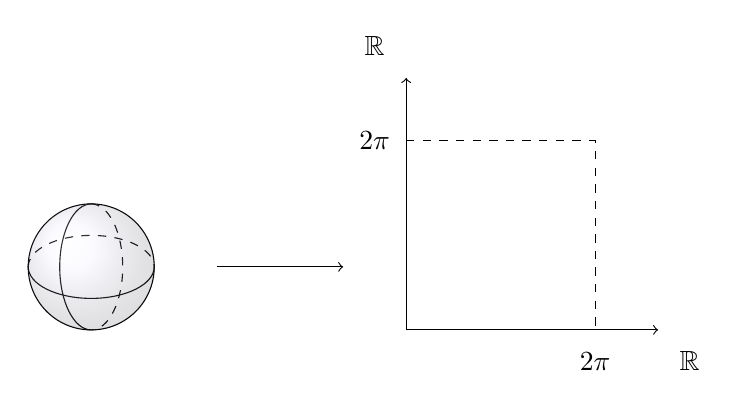
\begin{tikzpicture}[scale=0.8]
    \draw (-1,0) arc (180:360:1cm and 0.5cm);
    \draw[dashed] (-1,0) arc (180:0:1cm and 0.5cm);
    \draw (0,1) arc (90:270:0.5cm and 1cm);
    \draw[dashed] (0,1) arc (90:-90:0.5cm and 1cm);
    \draw (0,0) circle (1cm);
    \shade[ball color=blue!10!white,opacity=0.20] (0,0) circle (1cm);
    \draw[->] (2,0) -- (4,0);
\draw[->] (5,-1) node (v1) {} -- (5,3);
\draw[->] (5,-1) -- (9,-1);
\draw[dashed] (5,2) -- (8,2) -- (8,-1);
\node at (4.5,3.5) {$\mathbb{R}$};
\node at (9.5,-1.5) {$\mathbb{R}$};
\node at (4.5,2) {$2\pi$};
\node at (8,-1.5) {$2\pi$};
\end{tikzpicture}
\end{center}
\caption{Illustration of the 3-dimensional hypersphere, with a search space of $\mathbb{R}^2$
\label{fig:searchInAngles}}
\end{figure}







\clearpage

\bibliography{BSc2014}
\bibliographystyle{apalike}

\clearpage

\begin{appendices}

\section{Experiments}
This appendix contains all of the included experiments from which we have derived our results. Each of the plots, depending on the number of experiments, will depict the mean scores of the experiments or the experiments themselves.\\
With each experiment, a table detailing the parameter values will be included for others who would want to reproduce these experiments. Depending on the optimizer (weather it is Cross Entropy or CMA), the table will contain some custom rows, unique for the specific algorithm.\\
Similar for all experiments is the 30 games played with the new mean of each generation to generate the learning curve.\\
The tables are formatted 
\begin{table}[h]
\centering
\begin{tabular}{l r}
Optimizer & CMA\\
Number of Evaluations & -\\
Number of Learning Games & -\\
Population size& -\\
Parent size & -\\
Games per Agent & -\\
Tetris Type & -\\
\hline
Recombination Type & -\\
Initial Sigma & -\\
 & \\
\end{tabular}
\quad
\begin{tabular}{l r}
Optimizer & Cross Entropy\\
Number of Evaluations & -\\
Number of Learning Games & -\\
Population size & -\\
Parent size & -\\
Games per Agent & -\\
Tetris Type & -\\
\hline
Sigma & -\\
Noise Type & -\\
Noise & -
\end{tabular}
\caption{Overview of the two table formats}
\end{table}

\clearpage

\subsection{Game Complexity \label{AppendixGameComplexity}}
Experiments to test if game complexity can be used for tuning the CMA and CE configurations.

\begin{table}[h]
\centering
\begin{tabular}{l r}
Optimizer & Cross Entropy\\
Number of Evaluations & 8000\\
Population size & 100\\
Parent size & 10\\
Games per Agent & 1\\
Tetris Type & Hard\\
\hline
Sigma & 100\\
Noise Type & No noise\\
Noise & -
\end{tabular}
\quad
\begin{tabular}{l r}
Optimizer & Cross Entropy\\
Number of Evaluations & 8000\\
Population size & 100\\
Parent size & 10\\
Games per Agent & 1\\
Tetris Type & Normal\\
\hline
Sigma & 100\\
Noise Type & No noise\\
Noise & -
\end{tabular}
\caption{Cross Entropy settings for testing game complexity}
\end{table}

\begin{table}[h]
\centering
\begin{tabular}{l r}
Optimizer & CMA\\
Number of Evaluations & 8000\\
Number of Learning Games & 30\\
Population size& 13\\
Parent size & 6\\
Games per Agent & 1\\
Tetris Type & Hard\\
\hline
Recombination Type & Superlinear\\
Initial Sigma & 1
\end{tabular}
\quad
\begin{tabular}{l r}
Optimizer & CMA\\
Number of Evaluations & 8000\\
Number of Learning Games & 30\\
Population size& 13\\
Parent size & 6\\
Games per Agent & 1\\
Tetris Type & Normal\\
\hline
Recombination Type & Superlinear\\
Initial Sigma & 1
\end{tabular}
\caption{CMA settings for testing game complexity}
\end{table}

\clearpage

\begin{figure}
	\centering
	\captionsetup[subfigure]{justification=centering}
    \begin{subfigure}[b]{0.49\textwidth}
    	\caption{CMA - Hard Tetris}
        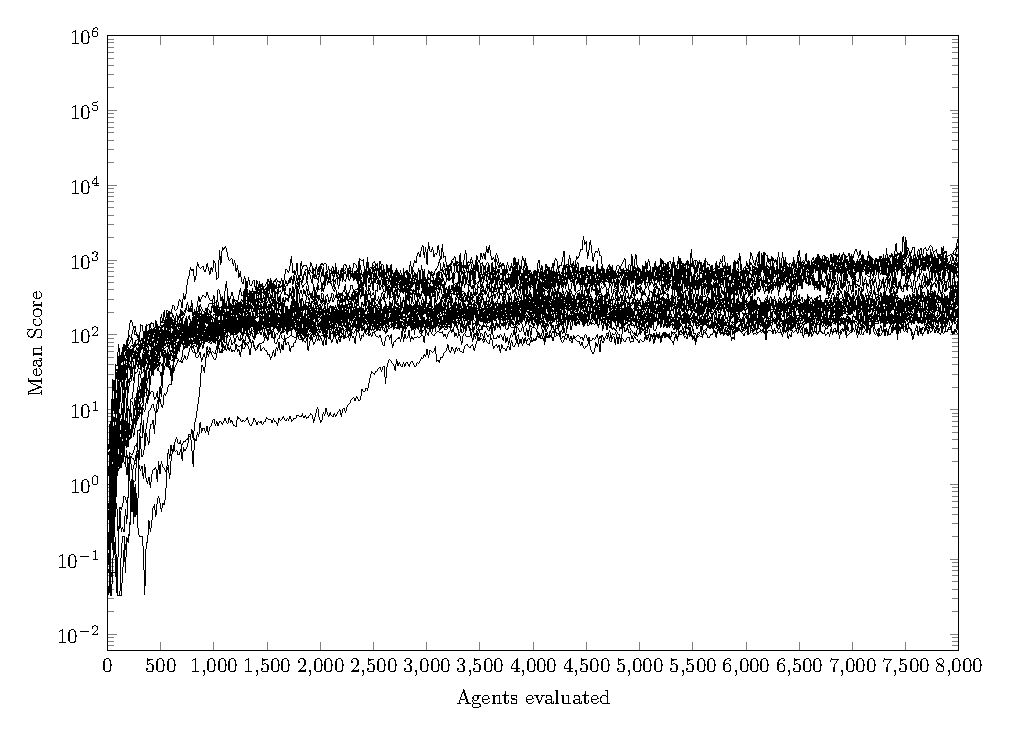
\includegraphics[width=\textwidth]{data/complexity/cma_hard/PlotFile.pdf}
    \end{subfigure} 
    \begin{subfigure}[b]{0.49\textwidth}
    	\caption{CMA - Normal Tetris}
        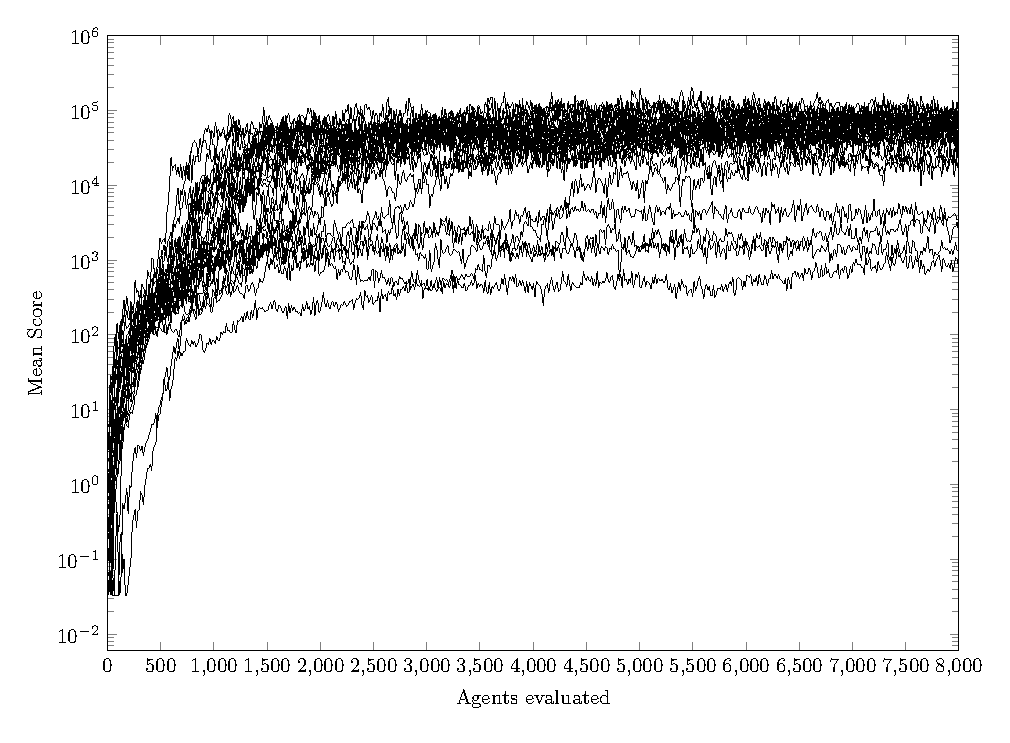
\includegraphics[width=\textwidth]{data/complexity/cma_normal/PlotFile.pdf}
    \end{subfigure}
    \begin{subfigure}[b]{0.49\textwidth}
    	\caption{Cross Entropy - Hard Tetris}
        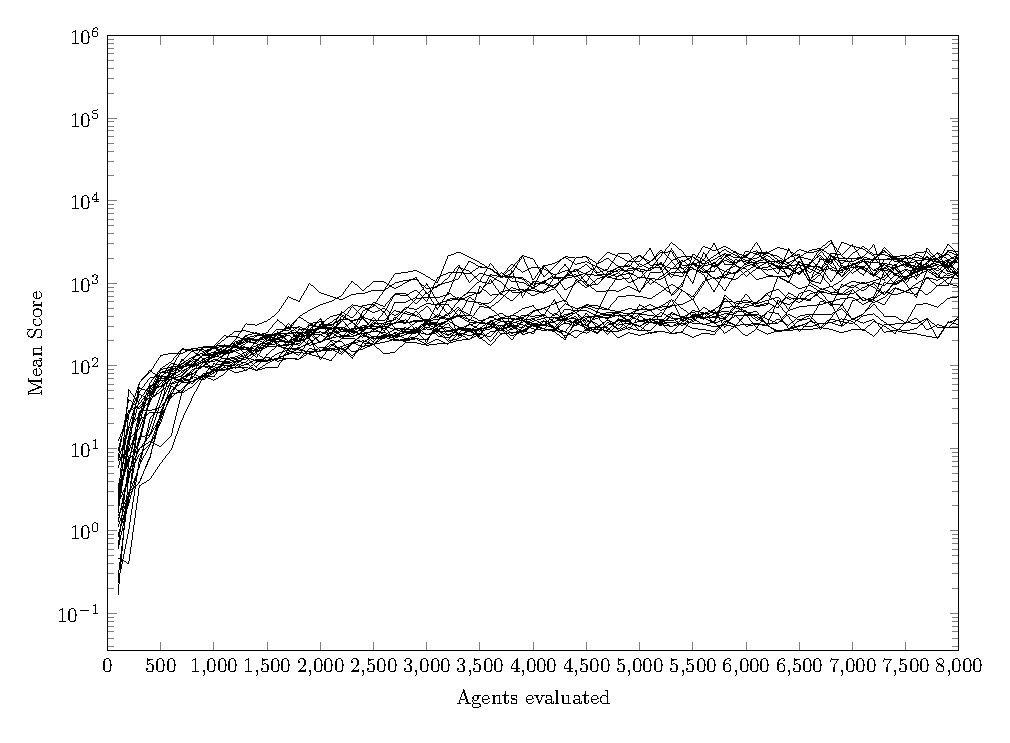
\includegraphics[width=\textwidth]{data/complexity/ce_hard/PlotFile.pdf}
    \end{subfigure}
    \begin{subfigure}[b]{0.49\textwidth}
    	\caption{Cross Entropy - Normal Tetris}
        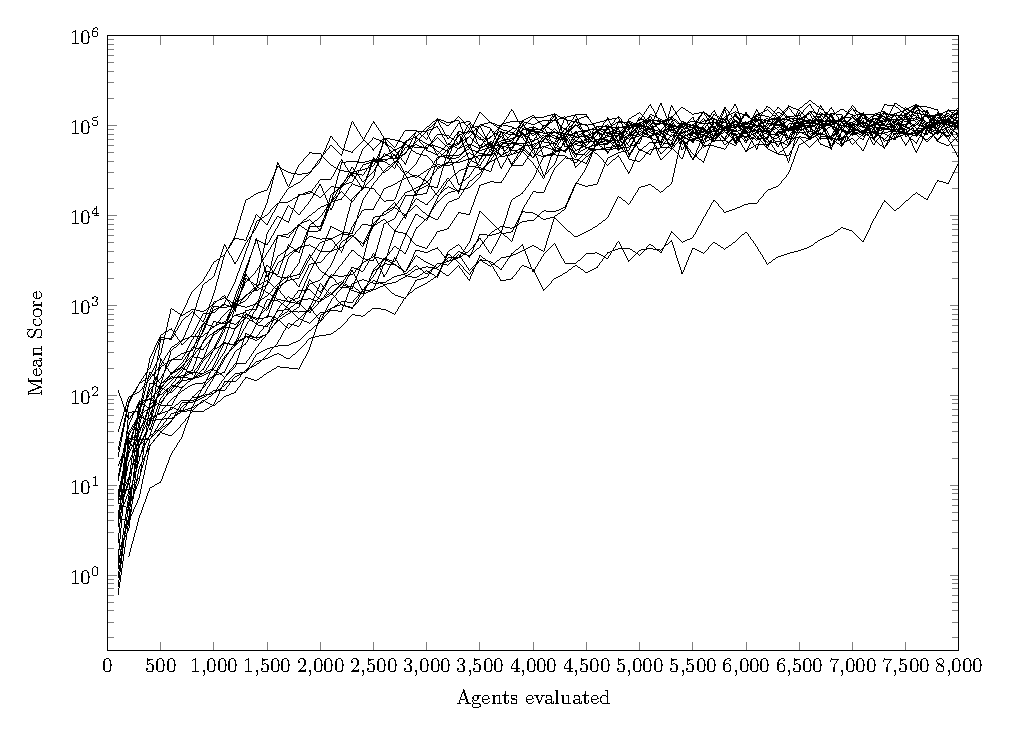
\includegraphics[width=\textwidth]{data/complexity/ce_normal/PlotFile.pdf}
    \end{subfigure}
    
    \caption{Complexity experiment results}
\end{figure}


\begin{table}[H]
\centering
\small
\begin{tabular}{c c c r r r r}
Tetris Type & Optimizer & mean & Q1 & Q2 & Q3\\
\hline
Hard & Cross Entropy & $1633.607$ & $1357.170$ & $1606.565$ & $1938.71$\\
Normal & Cross Entropy & $100059.463$ & $79357.440$ & $105999.500$ & $111047.500$\\
Hard & CMA & $449.352$ & $201.850$ & $300.300$ & $529.350$\\
Normal & CMA & $49760.161$ & $42528.740$ & $49915.700$ & $67764.729$\\
\end{tabular}
\caption{Experiment testing game Normal Tetris against Hard Tetris}
\end{table}

\begin{figure}[H]
\centering
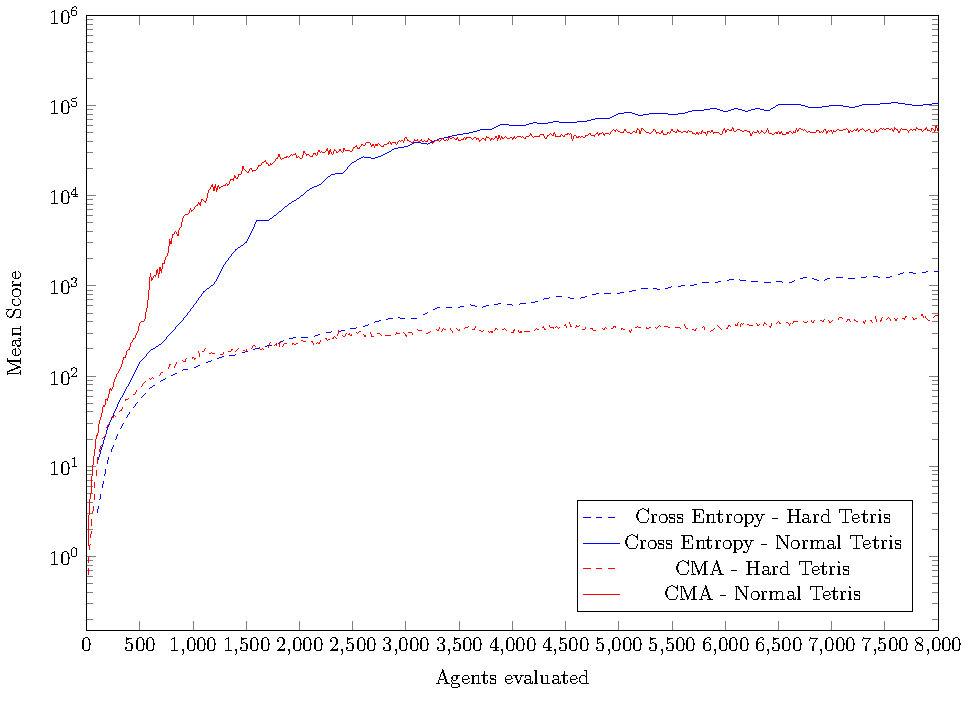
\includegraphics[scale=1]{data/complexity/mean/PlotFile.pdf}
\caption{Experiment testing game Normal Tetris against Hard Tetris}
\end{figure}

\clearpage

\subsection{Comparison - Comparison of featuresets}
Experiments to test Bertsekas and Dellacherie featuresets in regards to achieved score. This will tell if a different featureset affects the algorithms performance. 

\begin{table}[h]
\centering
\small
\caption{Shark stock CMA and Verified Cross Entropy}
\begin{tabular}{l r}
Optimizer & CMA\\
Number of Evaluations & 8000\\
Number of Learning Games & 30\\
Population size& 13\\
Parent size & 6\\
Games per Agent & 1\\
Tetris Type & Hard\\
\hline
Recombination Type & Superlinear\\
Initial Sigma & (what is stock)\\
\quad & \quad
\end{tabular}
\quad
\begin{tabular}{l r}
Optimizer & Cross Entropy\\
Number of Evaluations & 8000\\
Number of Learning Games & 30\\
Population size & 100\\
Parent size & 10\\
Games per Agent & 1\\
Tetris Type & Hard\\
\hline
Sigma & 100\\
Noise Type & Constant\\
Noise & 4
\end{tabular}
\end{table}

\comment{Add individual plots}

Used on the bertsekas and Dellacherie featuresets

\begin{figure}[H]
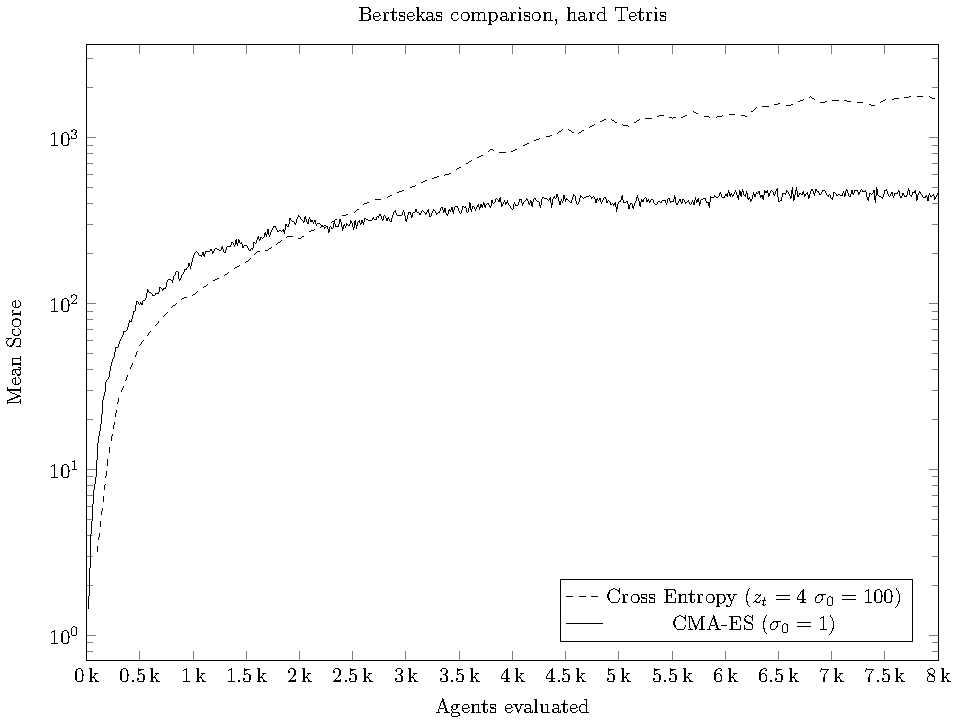
\includegraphics[scale=1]{plots/plotBertsekasCmaVsCEHardTetris}
\caption{Comparison between CMA-ES and Cross Entropy 
using hard Tetris and the Bertsekas featureset }
%\label{fig:featuresetCompareBertsekas}}
\end{figure}

\begin{figure}[H]
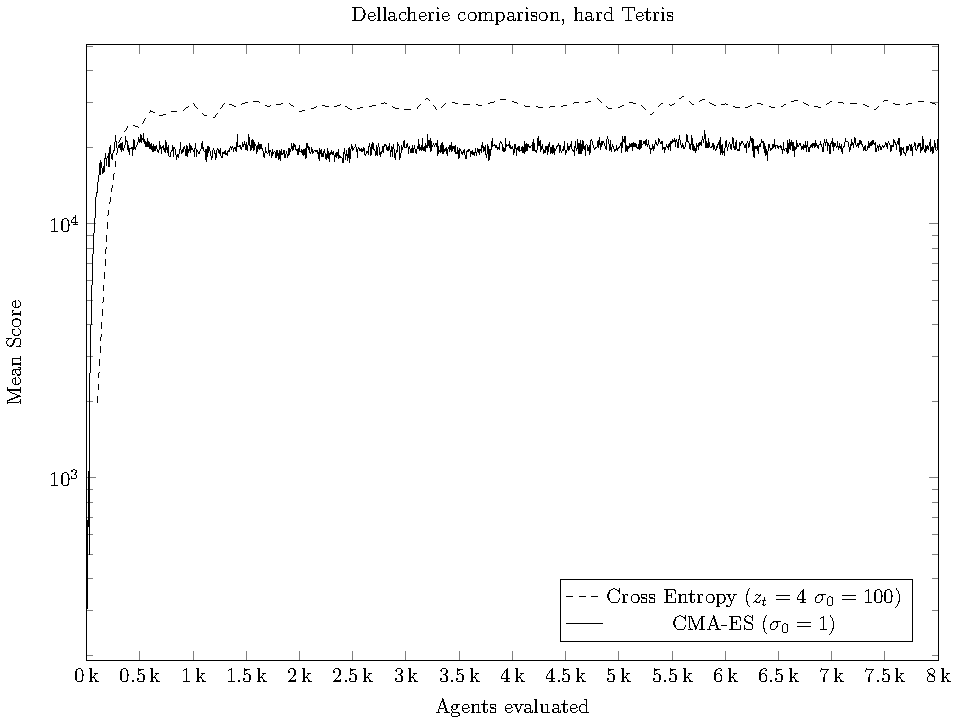
\includegraphics[scale=1]{plots/plotDellCmaVsCEHardTetris}
\caption{Comparison between CMA-ES and Cross Entropy 
using hard Tetris and the Dellacherie featureset}
%\label{fig:Dellacherie}}
\end{figure}

\clearpage

\subsection{Verification of Cross Entropy}
Using the same configuration as in "reference paper", we will reproduce the experiments to verify our implementation of Cross Entropy into the Shark Library.\\
\\
\begin{table}[h!]
\centering
\begin{tabular}{l r}
Optimizer & Cross Entropy\\
Number of Evaluations & 8000\\
Population size & 100\\
Parent size & 10\\
Games per Agent & 1\\
Tetris Type & Normal\\
\hline
Sigma & 100\\
Noise Type & No noise\\
Noise & -
\end{tabular}
\caption{Cross Entropy - No noise}
\end{table}

\begin{table}[h!]
\centering
\begin{tabular}{l r}
Optimizer & Cross Entropy\\
Number of Evaluations & 8000\\
Population size & 100\\
Parent size & 10\\
Games per Agent & 1\\
Tetris Type & Normal\\
\hline
Sigma & 100\\
Noise Type & Constant\\
Noise & 4
\end{tabular}
\caption{Cross Entropy - Constant noise}
\end{table}

\begin{table}[h!]
\centering
\begin{tabular}{l r}
Optimizer & Cross Entropy\\
Number of Evaluations & 8000\\
Population size & 100\\
Parent size & 10\\
Games per Agent & 1\\
Tetris Type & Normal\\
\hline
Sigma & 100\\
Noise Type & Linear decreasing\\
Noise & $max \left( 5 - \frac{t}{10}, 0 \right)$
\end{tabular}
\caption{Cross Entropy - Linear decreasing noise}
\end{table}

\clearpage

\begin{figure}[H]
\begin{center}
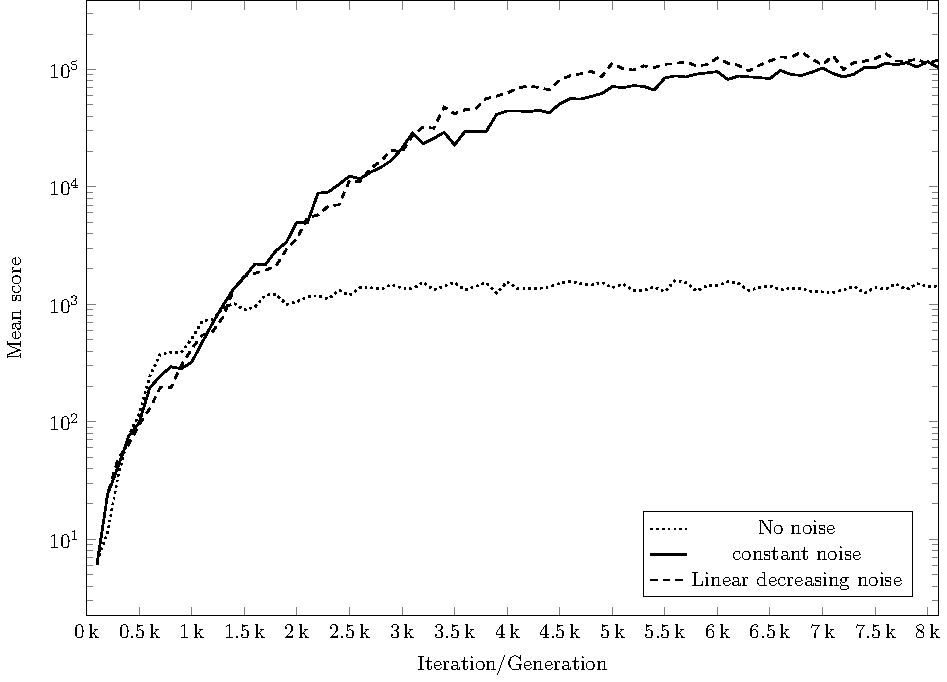
\includegraphics[scale=1]{plots/meansPlot}
\end{center}
\caption{Cross-Entropy mean performance}
\end{figure}

\clearpage
\begin{figure}[H]
\begin{center}
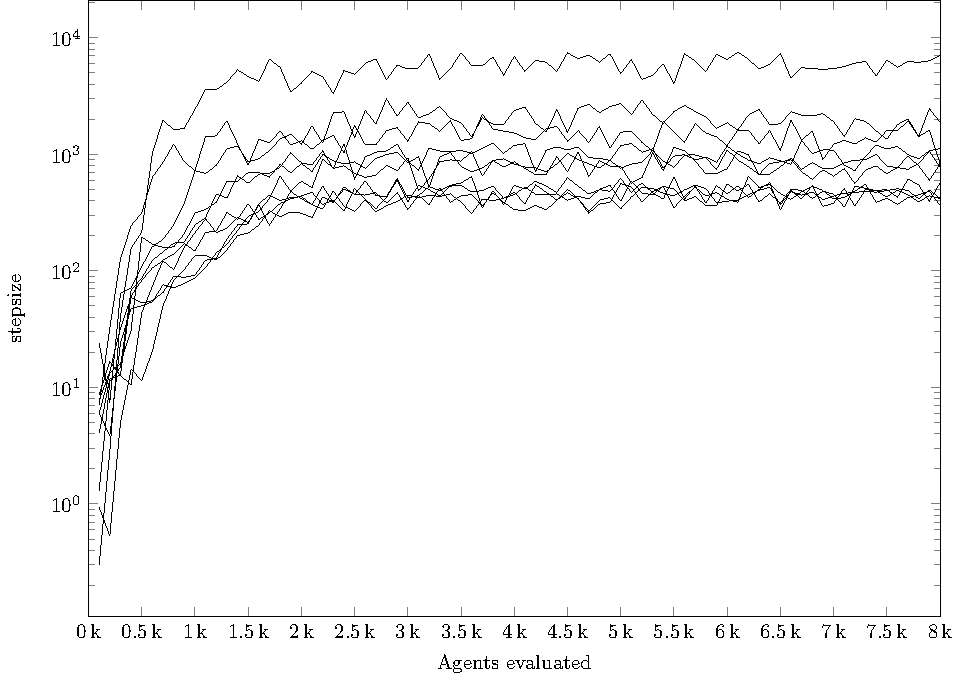
\includegraphics[scale=0.48]{plots/noNoisePlot}
\end{center}
\caption{No noise}
\end{figure}
\begin{figure}[H]
\begin{center}
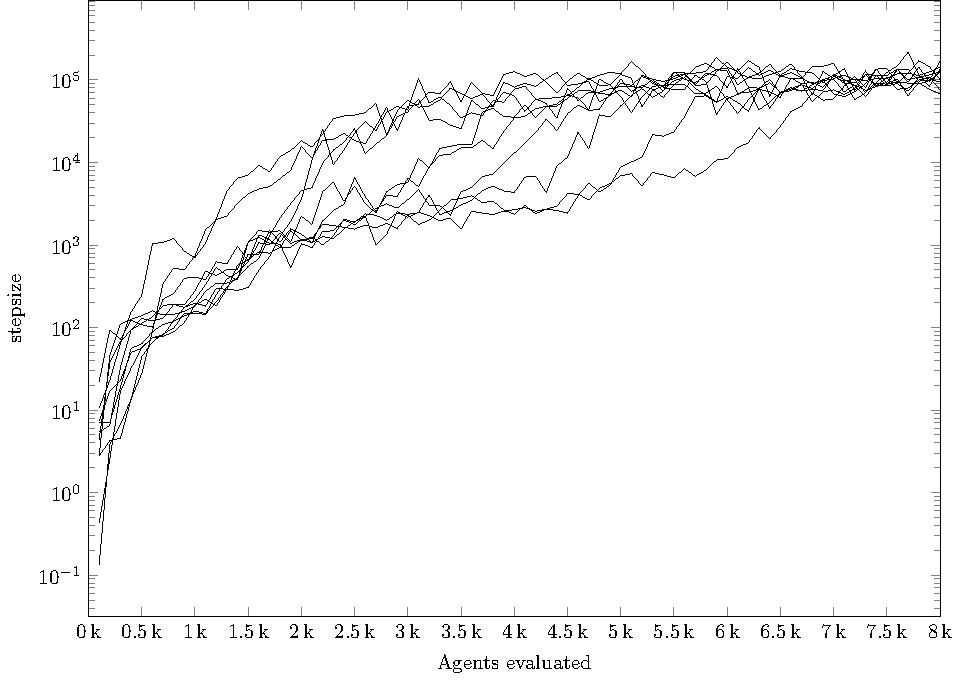
\includegraphics[scale=0.48]{plots/constantNoisePlot}
\end{center}
\caption{Constant noise}
\end{figure}
\begin{figure}[H]
\begin{center}
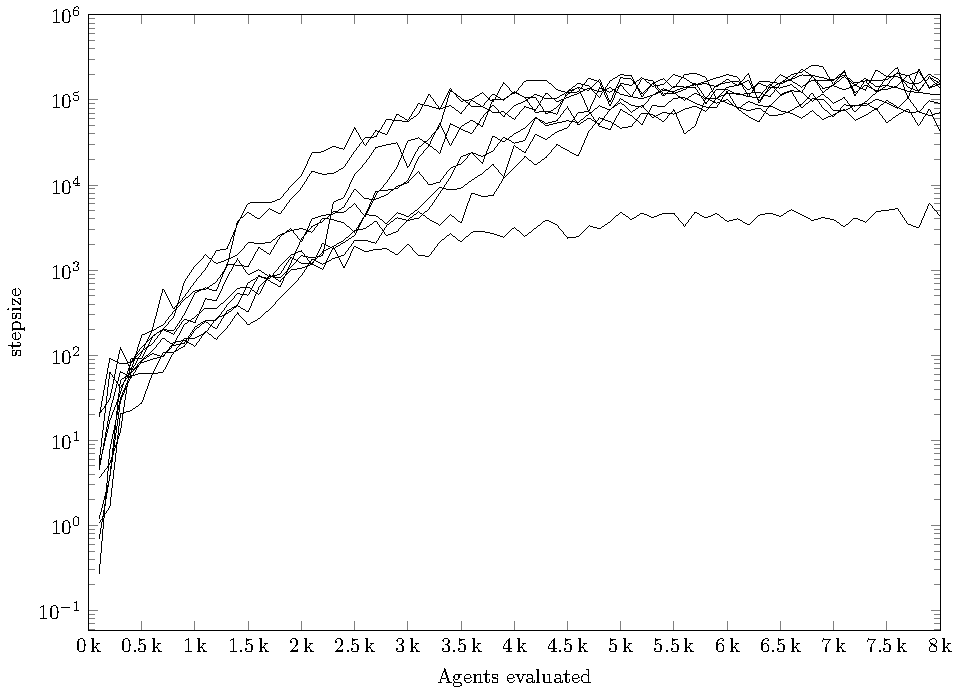
\includegraphics[scale=0.48]{plots/linearNoisePlot}
\end{center}
\caption{Linear decreasing noise}
\end{figure}


\clearpage

\subsection{Population and selection size}
\comment{Update plots and quantile table}\\
We want to investigate if there exists a better configuration than the 100/10 which was also previously used by other researchers.\\
In Cross Entropy for the Tetris problem, 10 \% Parent selection is used as standard. However, we will also test 50 \% Parent selection is a configuration from CMA which we will also test.\\
The general testing parameters are as follows
\begin{table}[h]
\centering
\begin{tabular}{l r}
Optimizer & Cross Entropy\\
Number of Evaluations & 8000\\
Population size & See table \ref{CEPopulationParentSize}\\
Parent size & See table \ref{CEPopulationParentSize}\\
Games per Agent & 1\\
Tetris Type & Normal\\
\hline
Sigma & 100\\
Noise Type & Constant\\
Noise & 4
\end{tabular}
\caption{General setup for Population/Parent size}
\end{table}

with the following population/Parent size

\begin{table}[h]
\centering
\begin{tabular}{l l}
Population size & Parent size\\
\hline
13 & 1\\
13 & 3\\
13 & 5\\
22 & 2\\
22 & 5\\
22 & 11\\
50 & 5\\
50 & 12\\
50 & 25\\
100 & 10\\
100 & 25\\
100 & 50\\
200 & 20\\
200 & 50\\
200 & 100
\end{tabular}
\caption{Population/Parent size \label{CEPopulationParentSize}}
\end{table}

INSERT PLOTS HERE.\\
\\
quantile table and two graphs over the mean plots of 10 \% and 50 \% Parent size

\clearpage

\begin{figure}[H]
\centering
\begin{tabular}{r r | r r r r}
population & offspring & mean & Q1 & Q2 & Q3\\
\hline
13 & $10\%$  & 1585,3     & 93,0      & 113,5        & 220,7\\
13 & $25\%$  & 30.496,9   & 15.222,1  & 20.264,2     & 39.019,8\\
13 & $50\%$  & 39.824,2   & 26.457,0  & 33.663,4     & 49.743,7\\
22 & $10\%$  & 35.841,6   & 20.391,9  & 42.045,5     & 48.464,6\\
22 & $25\%$  & 80.884,9   & 56.042,5  & 71.900,2     & 78.653,4\\
22 & $50\%$  & 52.887,4   & 23.531,9  & 42.161,0     & 83.144,1\\
50 & $10\%$  & 95,623,1   & 82.738,9  & 93.388,9     & 111.351,5\\
50 & $25\%$  & 110.525,0  & 103.128,1 & 111.195,5    & 121.974,4\\
50 & $50\%$  & 69.130,7   & 52.511,0  & 64.351,6     & 91.488,6\\
100 & $10\%$ & 115.868,7  & 84.368,5  & 122.238,5    & 146.457,0\\
100 & $25\%$ & 70.011,1   & 58.008,0  & 69.588,2     & 80.432,7\\
100 & $50\%$ & 22.910,4   & 4.037,7   & 14.353,7     & 47.215,9\\
200 & $10\%$ & 85.181,7   & 45.201,5  & 96.803,1     & 117.578,0\\
200 & $25\%$ & 32.894,6   & 8688,7    & 25.333,1     & 58.434,8\\
200 & $50\%$ & 946,4      & 585,0     & 802,5        & 1.267,7
\end{tabular}
\caption{Cross Entropy configuration test}
\end{figure}


The plots from the configuration of cross entropy.
All plots shows the numbers of games played along the x-axis
and the mean score of the centroid agent along the y-axis.

\begin{tabular}{@{}l@{}l@{}}
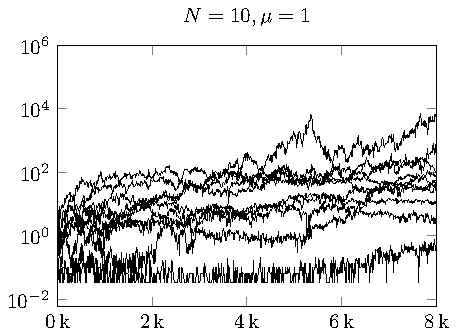
\includegraphics[scale=1]{plots/ce_ConstantNoise_l10_o1_all} &
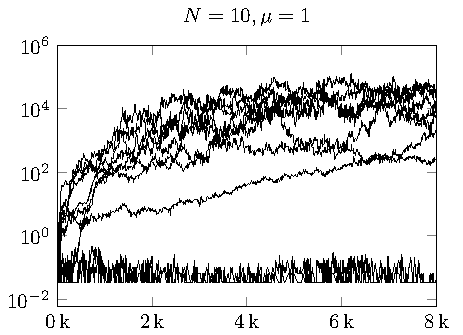
\includegraphics[scale=1]{plots/ce_ConstantNoise_l10_o5_all}
\end{tabular}

\begin{tabular}{@{}l@{}l@{}}
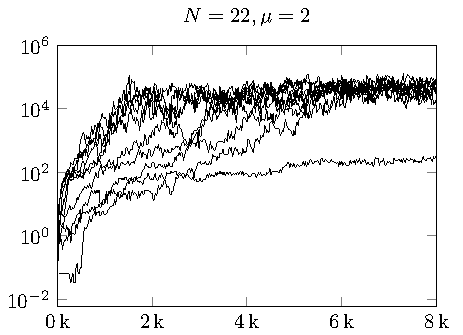
\includegraphics[scale=1]{plots/ce_ConstantNoise_l22_o2_all}&
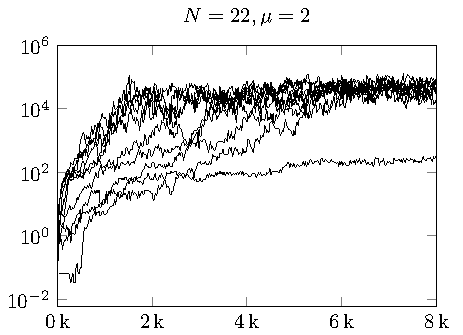
\includegraphics[scale=1]{plots/ce_ConstantNoise_l22_o2_all}
\end{tabular}

\begin{tabular}{@{}l@{}l@{}}
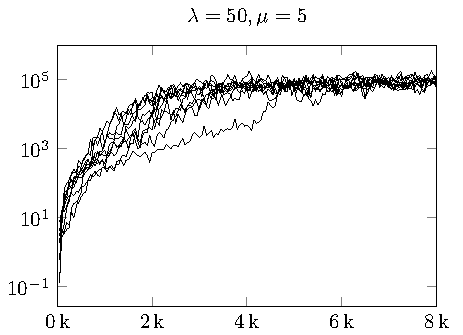
\includegraphics[scale=1]{plots/ce_ConstantNoise_l50_o5_all} &
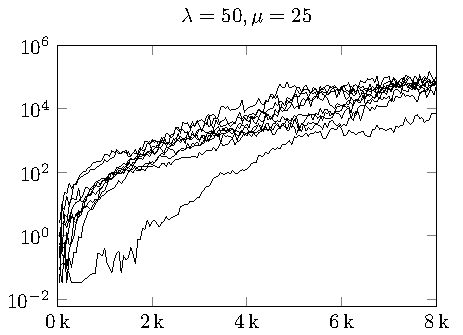
\includegraphics[scale=1]{plots/ce_ConstantNoise_l50_o25_all}
\end{tabular}

\begin{tabular}{@{}l@{}l@{}}
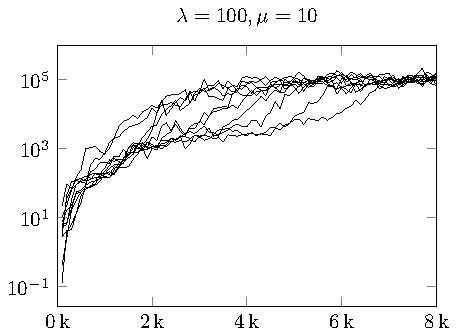
\includegraphics[scale=1]{plots/ce_ConstantNoise_l100_o10_all} &
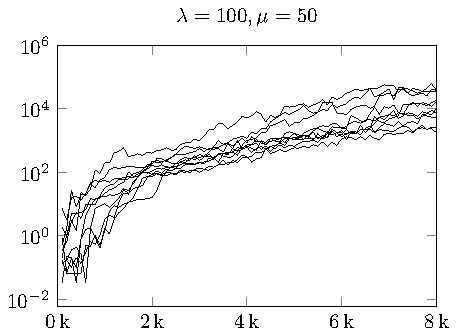
\includegraphics[scale=1]{plots/ce_ConstantNoise_l100_o50_all}
\end{tabular}

\begin{tabular}{@{}l@{}l@{}}
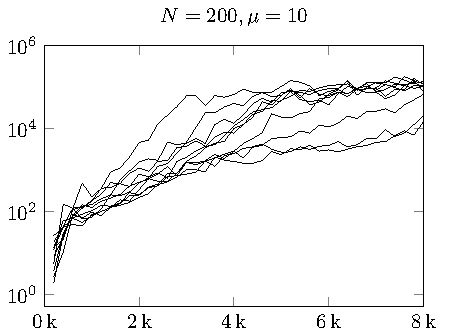
\includegraphics[scale=1]{plots/ce_ConstantNoise_l200_o20_all} &
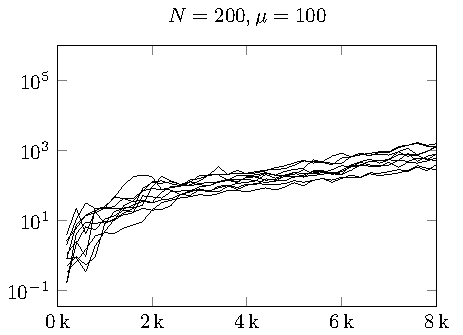
\includegraphics[scale=1]{plots/ce_ConstantNoise_l200_o100_all}
\end{tabular}


\clearpage

\subsection{Optimal settings for Cross Entropy - Games per agent \label{appendixCEPopulationParent}}
Experiment to determine the optimal number of games played per agent for best resulting score at lowest evaluation cost.

\begin{table}[h]
\centering
\caption{General setup for Population/Parent size}
\begin{tabular}{l r}
Optimizer & Cross Entropy\\
Number of Evaluations & 80000\\
Population size & See table \ref{GamesPerAgentCE}\\
Parent size & See table \ref{GamesPerAgentCE}\\
Games per Agent & See table \ref{GamesPerAgentCE}\\
Tetris Type & Hard\\
\hline
Sigma & 100\\
Noise Type & Constant\\
Noise & 4
\end{tabular}
\end{table}

with the following population/Parent size and number of games played per agent


\begin{table}[H]
\centering
\begin{tabular}{c c c}
Population Size & Parent size & Games per Agent\\
\hline
$12$ & $10\%$ & 1/3/5/7/10\\
$12$ & $25\%$ & 1/3/5/7/10\\
$12$ & $50\%$ & 1/3/5/7/10\\
$22$ & $10\%$ & 1/3/5/7/10\\
$22$ & $25\%$ & 1/3/5/7/10\\
$22$ & $50\%$ & 1/3/5/7/10\\
$50$ & $10\%$ & 1/3/5/7/10\\
$50$ & $25\%$ & 1/3/5/7/10\\
$50$ & $50\%$ & 1/3/5/7/10\\
$100$ & $10\%$ & 1/3/5/7/10\\
$100$ & $25\%$ & 1/3/5/7/10\\
$100$ & $50\%$ & 1/3/5/7/10\\
$200$ & $10\%$ & 1/3/5/7/10\\
$200$ & $25\%$ & 1/3/5/7/10\\
$200$ & $50\%$ & 1/3/5/7/10
\end{tabular}
\caption{Games per agent CE experiment setup}
%\label{GamesPerAgentCE}}
\end{table}

\clearpage

\begin{figure}
	\centering
	\captionsetup[subfigure]{justification=centering}
    \begin{subfigure}[b]{0.49\textwidth}
    	\caption{Population size 13, Parent size 1}
        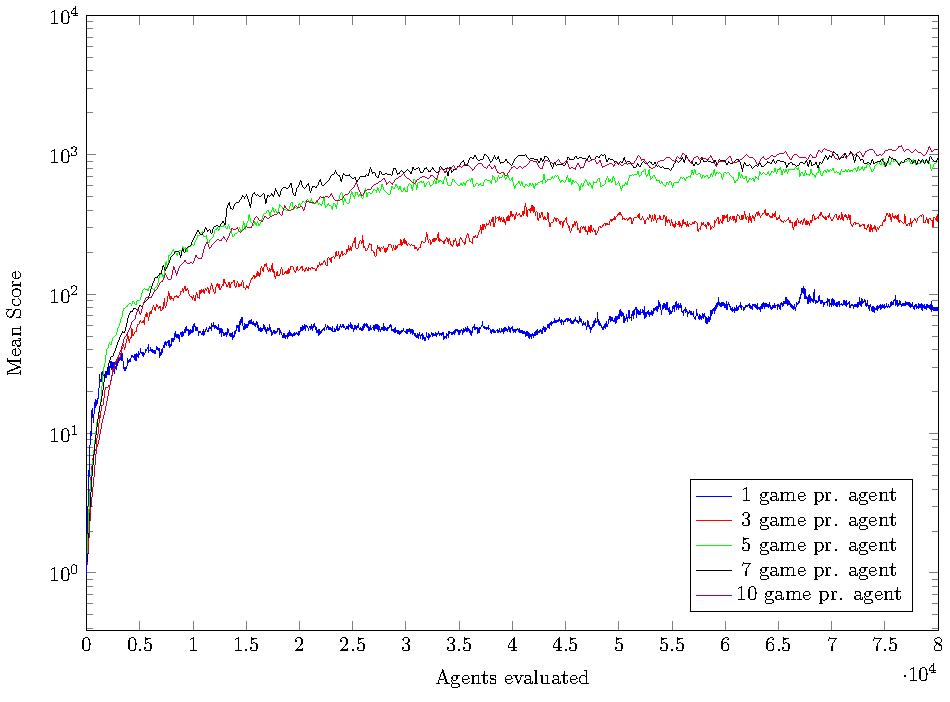
\includegraphics[width=\textwidth]{data/ce_population_offspring/13x_split/constant_l13_o1/mean/PlotFile.pdf}
    \end{subfigure} 
    \begin{subfigure}[b]{0.49\textwidth}
    	\caption{Population size 13, Parent size 3}
        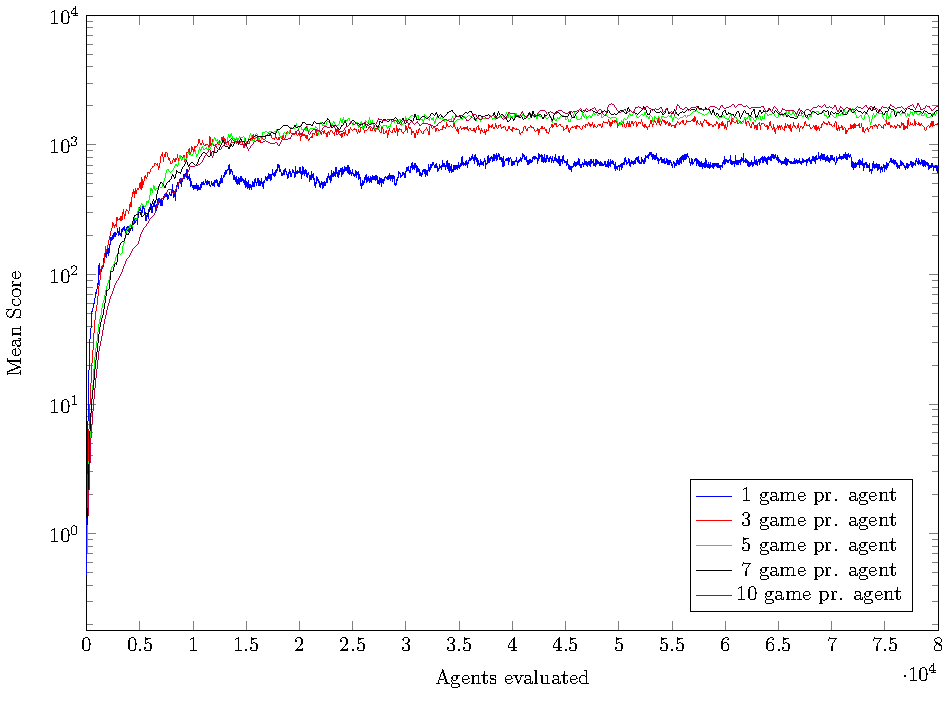
\includegraphics[width=\textwidth]{data/ce_population_offspring/13x_split/constant_l13_o3/mean/PlotFile.pdf}
    \end{subfigure}
    \begin{subfigure}[b]{0.49\textwidth}
    	\caption{Population size 13, Parent size 6}
        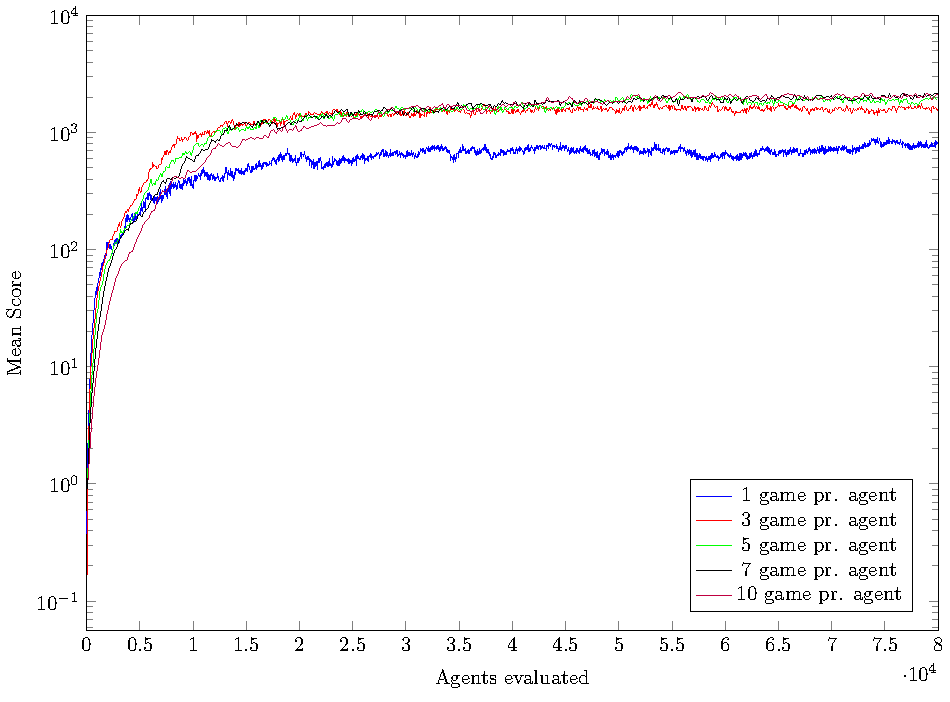
\includegraphics[width=\textwidth]{data/ce_population_offspring/13x_split/constant_l13_o6/mean/PlotFile.pdf}
    \end{subfigure}
    \begin{subfigure}[b]{0.49\textwidth}
    	\caption{Population size 22, Parent size 2}
        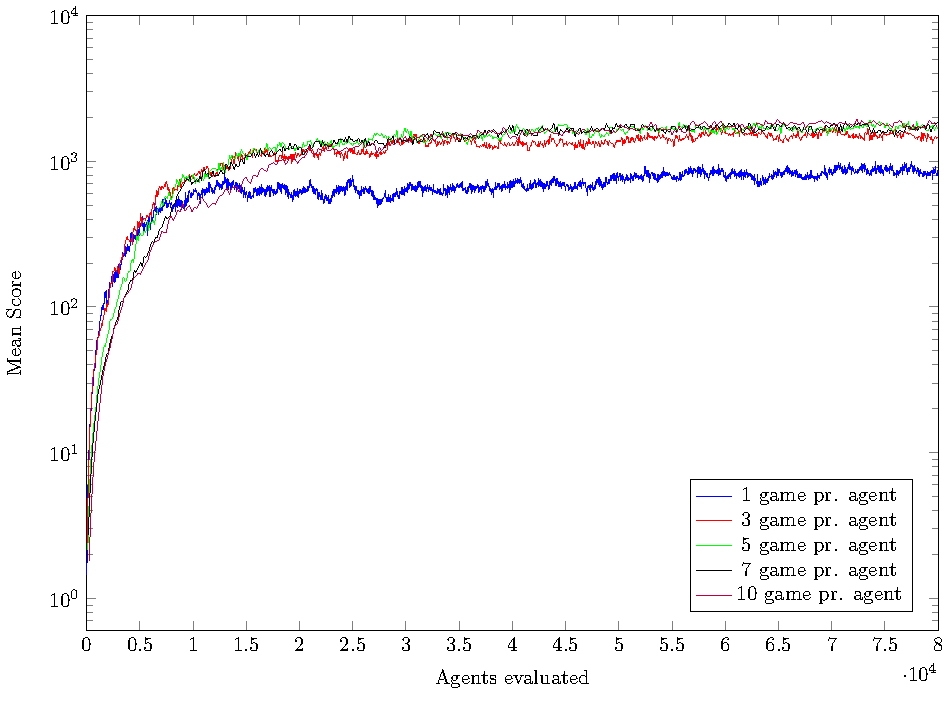
\includegraphics[width=\textwidth]{data/ce_population_offspring/22x_split/constant_l22_o2/mean/PlotFile.pdf}
    \end{subfigure}
    \begin{subfigure}[b]{0.49\textwidth}
    	\caption{Population size 22, Parent size 5}
        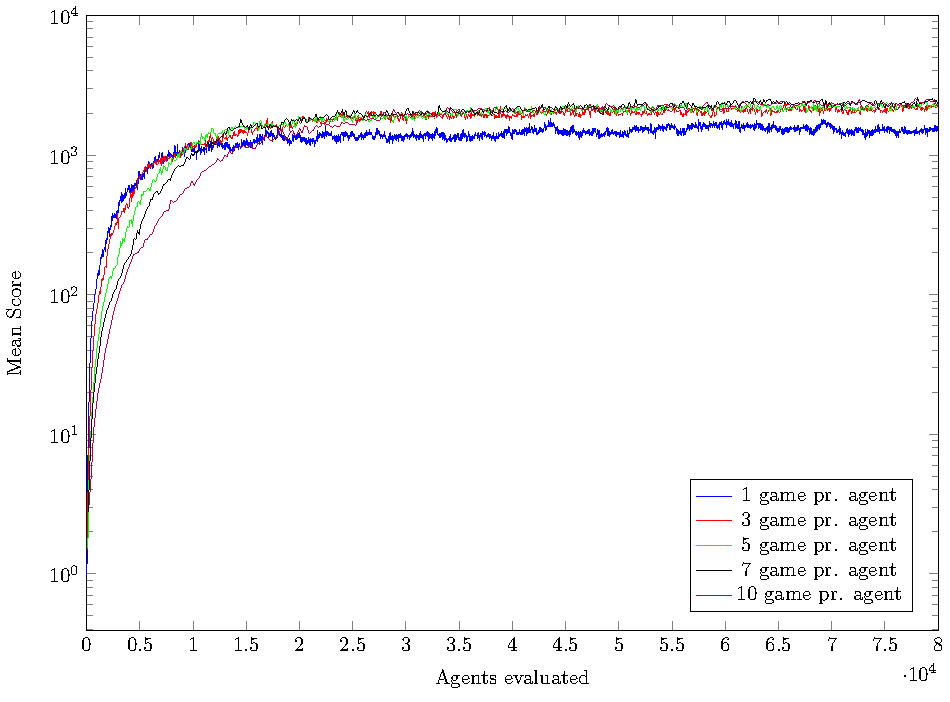
\includegraphics[width=\textwidth]{data/ce_population_offspring/22x_split/constant_l22_o5/mean/PlotFile.pdf}
    \end{subfigure}
    \begin{subfigure}[b]{0.49\textwidth}
    	\caption{Population size 22, Parent size 11}
        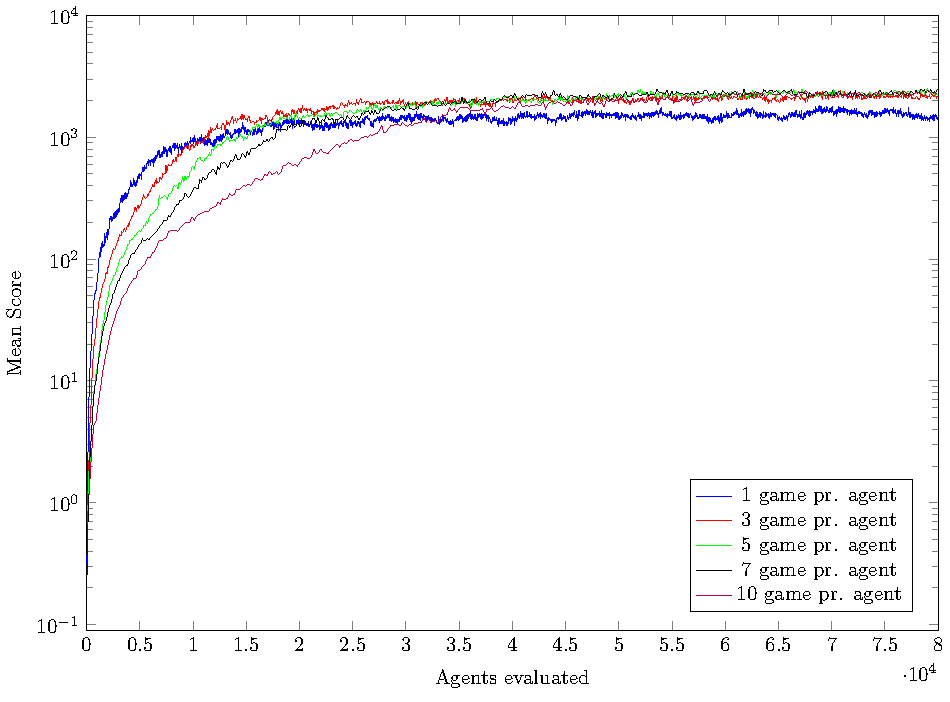
\includegraphics[width=\textwidth]{data/ce_population_offspring/22x_split/constant_l22_o11/mean/PlotFile.pdf}
    \end{subfigure}
    
    \caption{Mean results for population size 12 and 22 with parent sizes $10 \% , 25 \%$ and $50 \%$}
\end{figure}

\clearpage

\begin{figure}
	\centering
	\captionsetup[subfigure]{justification=centering}
    \begin{subfigure}[b]{0.49\textwidth}
    	\caption{Population size 50, Parent size 5}
        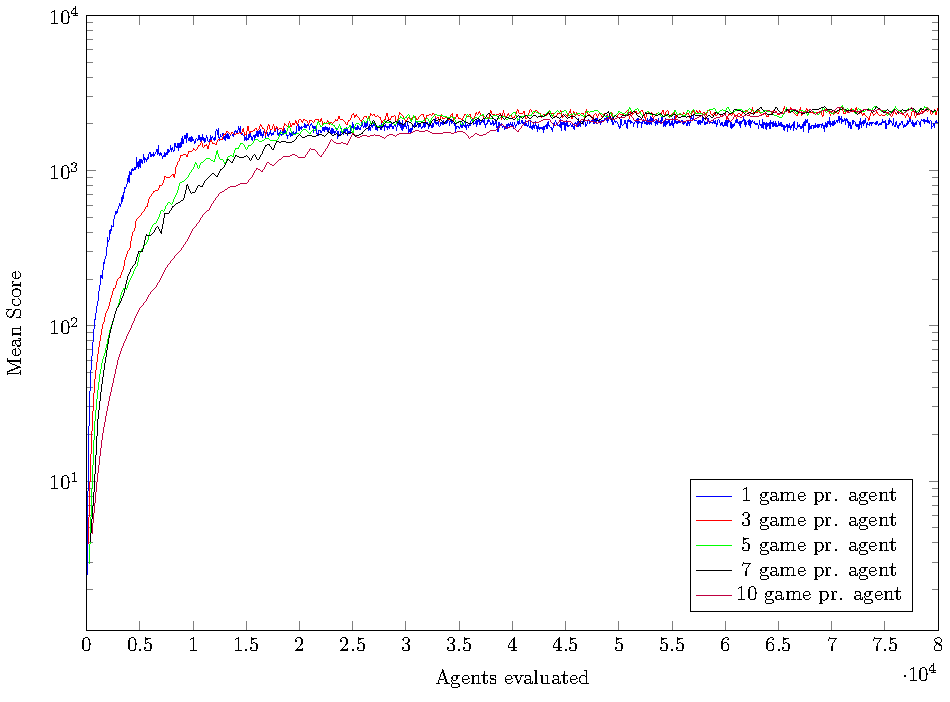
\includegraphics[width=\textwidth]{data/ce_population_offspring/50x_split/constant_l50_o5/mean/PlotFile.pdf}
    \end{subfigure} 
    \begin{subfigure}[b]{0.49\textwidth}
    	\caption{Population size 50, Parent size 12}
        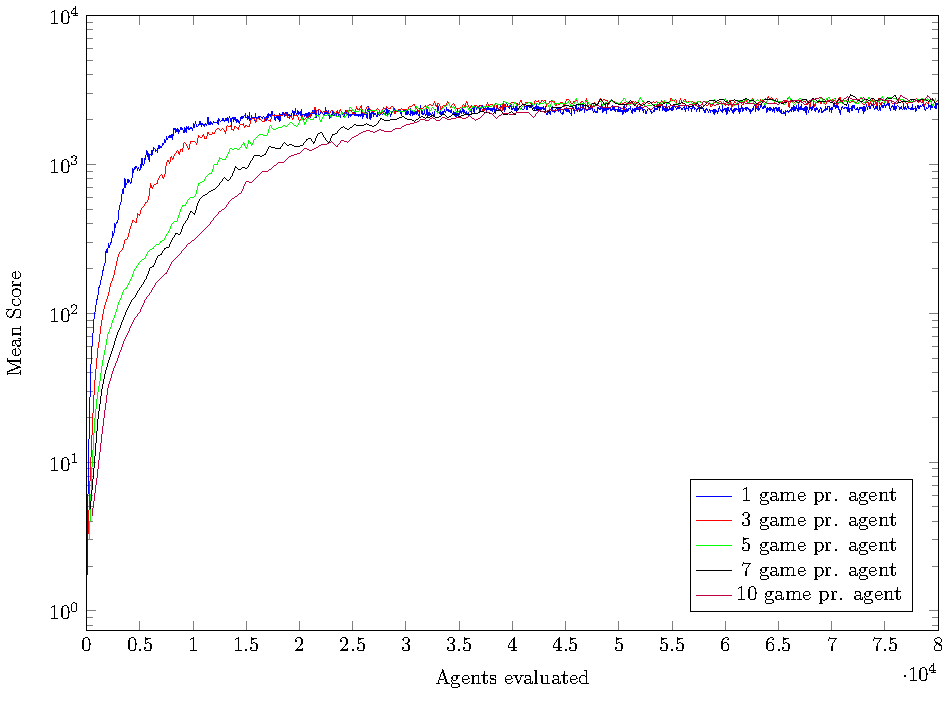
\includegraphics[width=\textwidth]{data/ce_population_offspring/50x_split/constant_l50_o12/mean/PlotFile.pdf}
    \end{subfigure}
    \begin{subfigure}[b]{0.49\textwidth}
    	\caption{Population size 50, Parent size 25}
        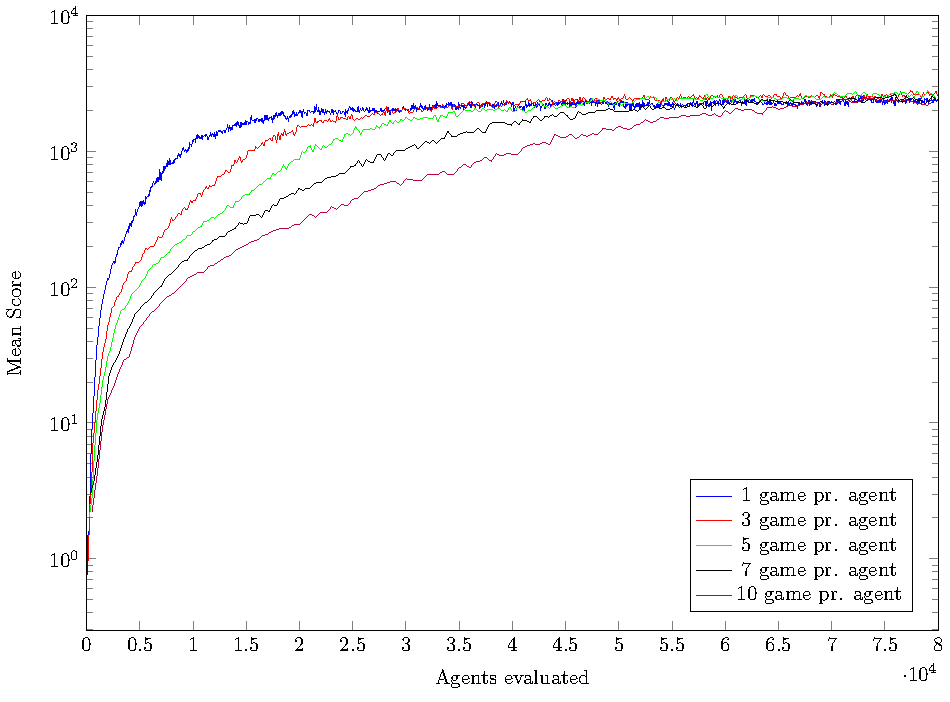
\includegraphics[width=\textwidth]{data/ce_population_offspring/50x_split/constant_l50_o25/mean/PlotFile.pdf}
    \end{subfigure}
    \begin{subfigure}[b]{0.49\textwidth}
    	\caption{Population size 100, Parent size 10}
        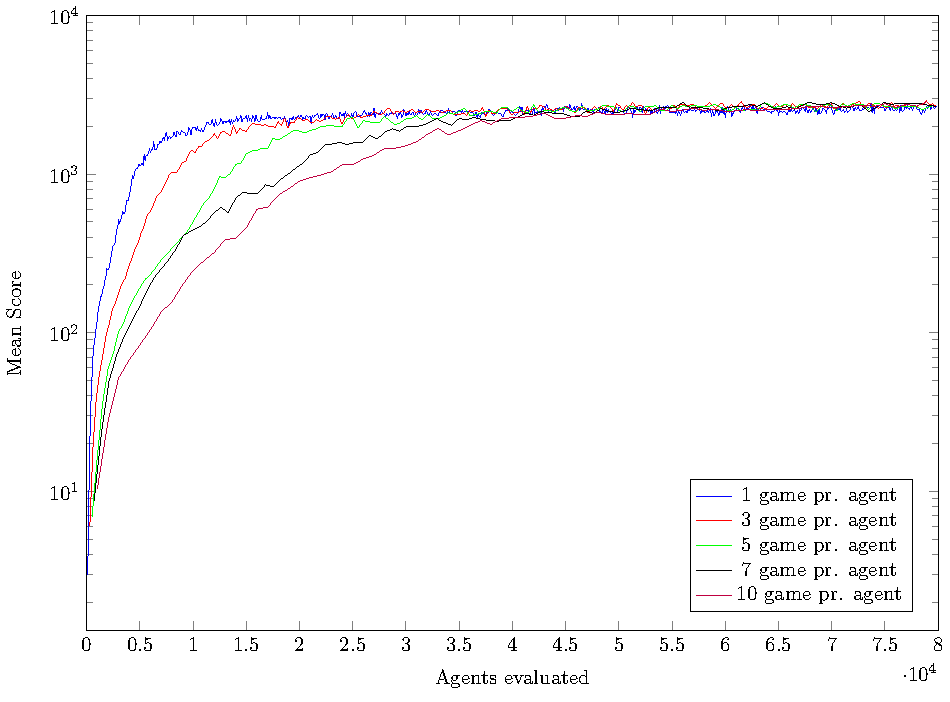
\includegraphics[width=\textwidth]{data/ce_population_offspring/100x_split/constant_l100_o10/mean/PlotFile.pdf}
    \end{subfigure}
    \begin{subfigure}[b]{0.49\textwidth}
    	\caption{Population size 100, Parent size 25}
        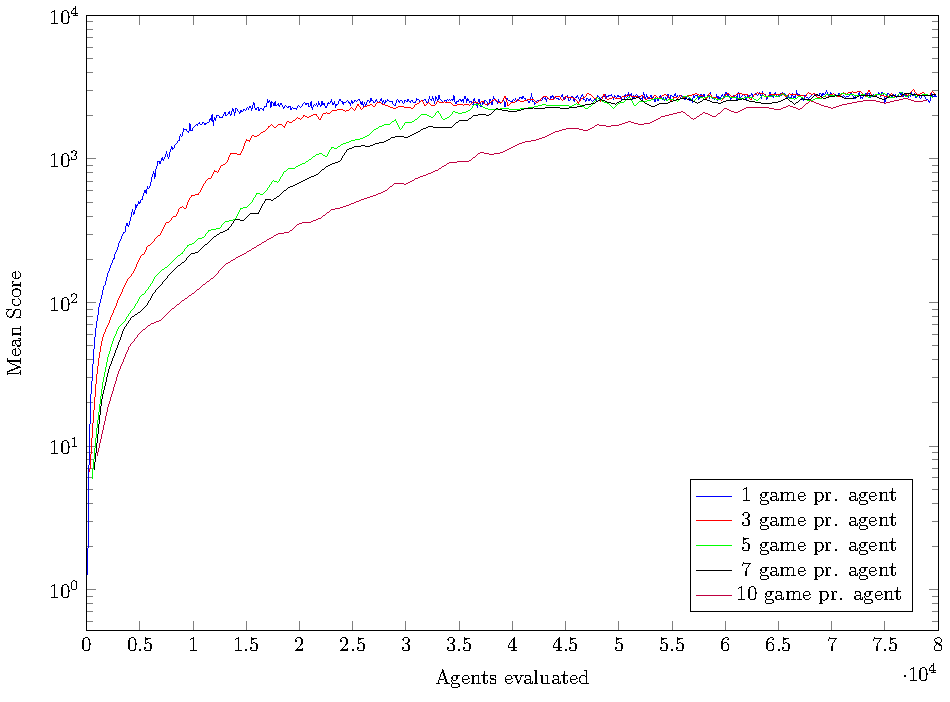
\includegraphics[width=\textwidth]{data/ce_population_offspring/100x_split/constant_l100_o25/mean/PlotFile.pdf}
    \end{subfigure}
    \begin{subfigure}[b]{0.49\textwidth}
    	\caption{Population size 100, Parent size 50}
        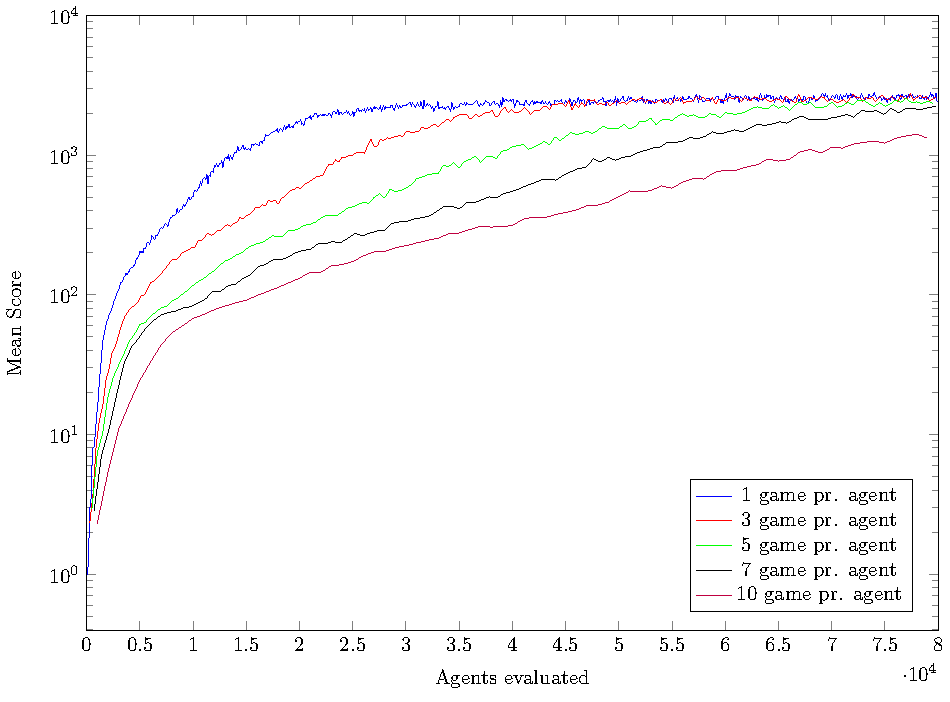
\includegraphics[width=\textwidth]{data/ce_population_offspring/100x_split/constant_l100_o50/mean/PlotFile.pdf}
    \end{subfigure}
    
    \caption{Mean results for population size 50 and 100 with parent sizes $10 \% , 25 \%$ and $50 \%$}
\end{figure}

\clearpage

\begin{figure}
	\captionsetup[subfigure]{justification=centering}
    \begin{subfigure}[b]{0.49\textwidth}
    	\caption{Population size 200, Parent size 20}
        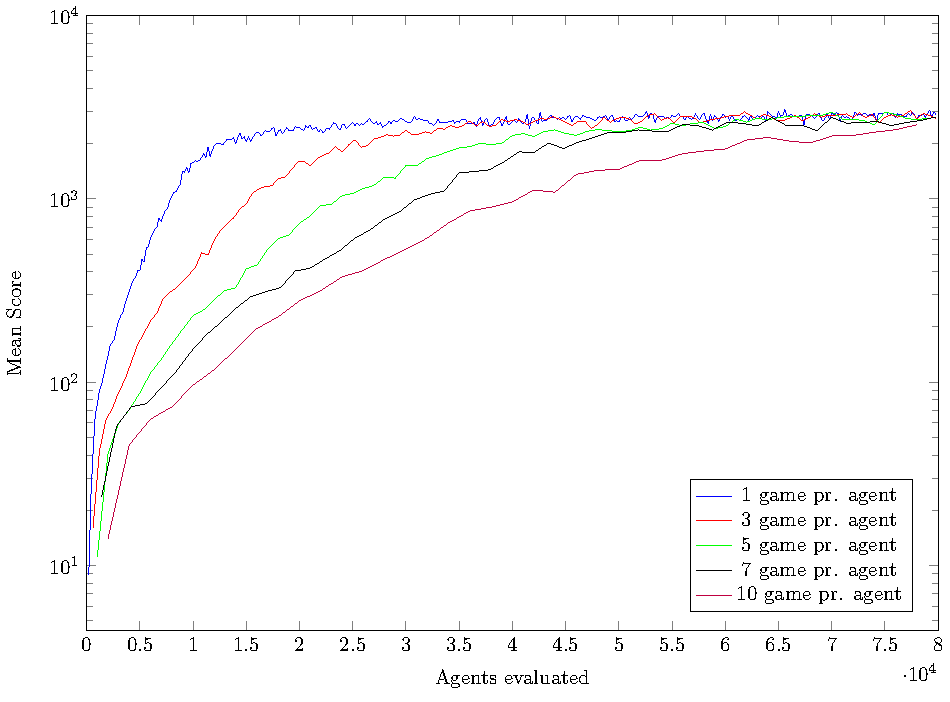
\includegraphics[width=\textwidth]{data/ce_population_offspring/200x_split/constant_l200_o20/mean/PlotFile.pdf}
    \end{subfigure} 
    \begin{subfigure}[b]{0.49\textwidth}
    	\caption{Population size 200, Parent size 50}
        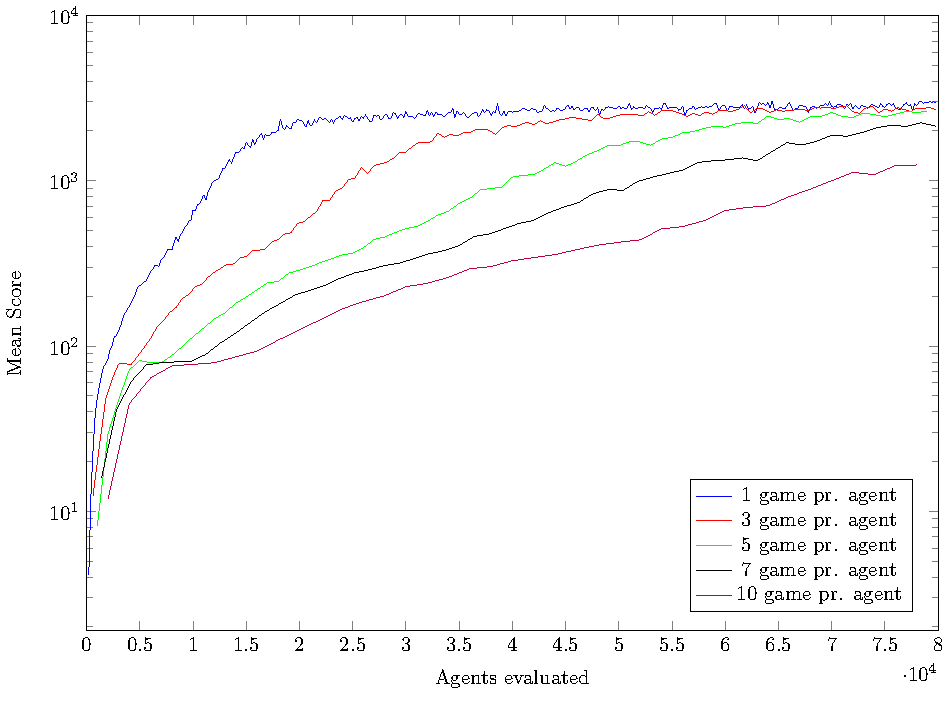
\includegraphics[width=\textwidth]{data/ce_population_offspring/200x_split/constant_l200_o50/mean/PlotFile.pdf}
    \end{subfigure}
    \begin{subfigure}[b]{0.49\textwidth}
    	\caption{Population size 200, Parent size 100}
        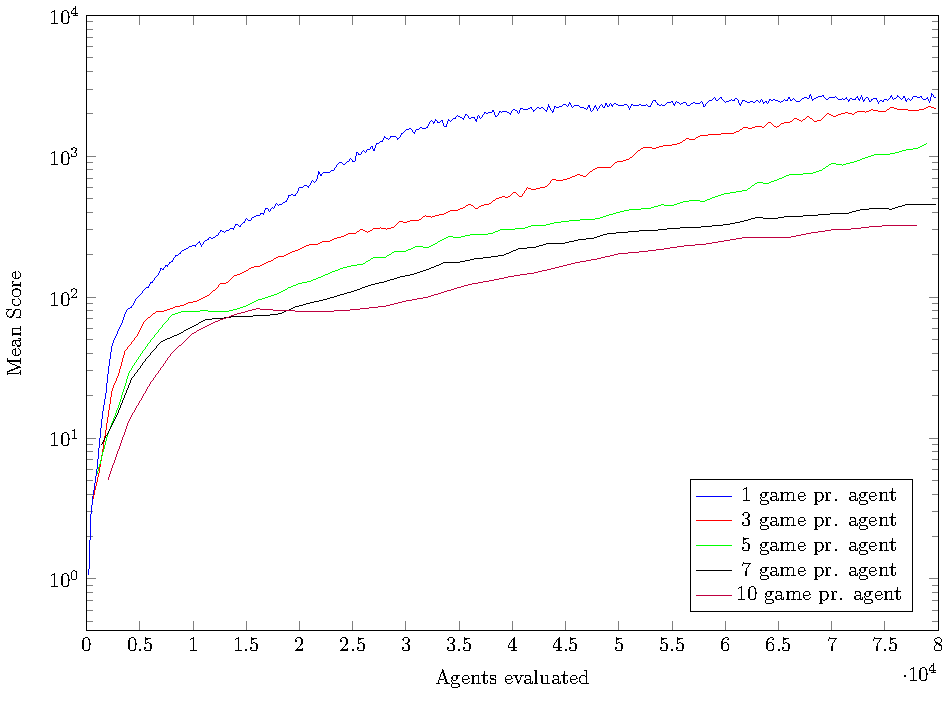
\includegraphics[width=\textwidth]{data/ce_population_offspring/200x_split/constant_l200_o100/mean/PlotFile.pdf}
    \end{subfigure}
    
    \caption{Mean results for population size 200 with parent sizes $10 \% , 25 \%$ and $50 \%$}
\end{figure}

\clearpage

\begin{table}[H]
\centering
\small
\begin{tabular}{c c c r r r r}
Population & Parent & Games per Agent & mean & Q1 & Q2 & Q3\\
\hline
$13$ & $1$ & 1 & $76.402$ & $46.143$ & $58.850$ & $87.786$\\
$13$ & $1$ & 3 & $329.847$ & $180.787$ & $266.633$ & $418.630$\\
$13$ & $1$ & 5 & $870.593$ & $648.593$ & $870.466$ & $1047.998$\\
$13$ & $1$ & 7 & $951.487$ & $646.383$ & $915.418$ & $1130.101$\\
\hdashline
$13$ & $1$ & 10 & $1098.654$ & $834.683$ & $939.150$ & $1270.262$\\
\hdashline
$13$ & $3$ & 1 & $681.930$ & $451.493$ & $615.583$ & $777.900$\\
$13$ & $3$ & 3 & $1485.366$ & $1260.690$ & $1497.965$ & $1582.008$\\
$13$ & $3$ & 5 & $1779.540$ & $1448.080$ & $1764.150$ & $2103.521$\\
$13$ & $3$ & 7 & $1844.008$ & $1635.631$ & $1790.465$ & $2025.209$\\
\hdashline
$13$ & $3$ & 10 & $1992.749$ & $1566.989$ & $1965.365$ & $2381.089$\\
\hdashline
$13$ & $6$ & 1 & $814.019$ & $598.073$ & $736.783$ & $966.0269$\\
$13$ & $6$ & 3 & $1595.290$ & $1219.319$ & $1504.700$ & $1870.699$\\
$13$ & $6$ & 5 & $1981.514$ & $1695.181$ & $1927.700$ & $2151.810$\\
\hdashline
$13$ & $6$ & 7 & $2173.595$ & $1818.110$ & $2105.500$ & $2398.201$\\
\hdashline
$13$ & $6$ & 10 & $2129.880$ & $1825.599$ & $2058.970$ & $2391.860$\\
\hdashline
\end{tabular}
\caption{population 12 - Cross Entropy}
\end{table}

\begin{table}[H]
\centering
\small
\begin{tabular}{c c c r r r r}
Population & Parent & Games per Agent & mean & Q1 & Q2 & Q3\\
\hline
$22$ & $2$ & 1 & $849.001$ & $542.797$ & $799.083$ & $1031.299$\\
$22$ & $2$ & 3 & $1442.883$ & $1276.870$ & $1437.550$ & $1541.938$\\
$22$ & $2$ & 5 & $1668.974$ & $1352.250$ & $1579.885$ & $1849.210$\\
\hdashline
$22$ & $2$ & 7 & $1843.644$ & $1575.732$ & $1860.815$ & $2112.678$\\
\hdashline
$22$ & $2$ & 10 & $1732.664$ & $1475.000$ & $1754.785$ & $2024.980$\\
$22$ & $5$ & 1 & $1485.692$ & $1202.661$ & $1561.635$ & $1661.268$\\
$22$ & $5$ & 3 & $2250.239$ & $2081.798$ & $2210.850$ & $2435.021$\\
\hdashline
$22$ & $5$ & 5 & $2371.793$ & $2013.168$ & $2412.815$ & $2708.931$\\
\hdashline
$22$ & $5$ & 7 & $2351.371$ & $1976.141$ & $2274.180$ & $2586.641$\\
$22$ & $5$ & 10 & $2266.329$ & $2010.798$ & $2175.850$ & $2365.220$\\
$22$ & $11$ & 1 & $1415.511$ & $1011.101$ & $1327.030$ & $1600.599$\\
$22$ & $11$ & 3 & $2168.012$ & $1966.552$ & $2119.100$ & $2456.230$\\
$22$ & $11$ & 5 & $2245.854$ & $2017.992$ & $2222.900$ & $2424.450$\\
\hdashline
$22$ & $11$ & 7 & $2463.227$ & $2091.090$ & $2384.230$ & $2702.740$\\
\hdashline
$22$ & $11$ & 10 & $2282.032$ & $1957.148$ & $2257.285$ & $2565.950$\\
\end{tabular}
\caption{population 22 - Cross Entropy}
\end{table}


\begin{table}[H]
\centering
\small
\begin{tabular}{c c c r r r r}
Population & Parent & Games per Agent & mean & Q1 & Q2 & Q3\\
\hline
$50$ & $5$ & 1 & $2060.069$ & $1731.441$ & $1967.465$ & $2076.389$\\
\hdashline
$50$ & $5$ & 3 & $2524.279$ & $2195.189$ & $2501.985$ & $2848.859$\\
\hdashline
$50$ & $5$ & 5 & $2418.023$ & $2283.708$ & $2388.770$ & $2639.078$\\
$50$ & $5$ & 7 & $2433.615$ & $2145.718$ & $2356.800$ & $2734.611$\\
$50$ & $5$ & 10 & $2341.267$ & $2104.480$ & $2252.570$ & $2418.809$\\
$50$ & $12$ & 1 & $2563.539$ & $2283.399$ & $2502.880$ & $2830.192$\\
$50$ & $12$ & 3 & $2702.266$ & $2322.849$ & $2565.365$ & $2841.160$\\
\hdashline
$50$ & $12$ & 5 & $2749.991$ & $2605.171$ & $2702.400$ & $2835.960$\\
\hdashline
$50$ & $12$ & 7 & $2527.792$ & $2287.091$ & $2476.965$ & $2758.970$\\
$50$ & $12$ & 10 & $2687.438$ & $2342.811$ & $2577.285$ & $2838.771$\\
$50$ & $25$ & 1 & $2396.866$ & $2115.161$ & $2357.980$ & $2664.099$\\
\hdashline
$50$ & $25$ & 3 & $2572.860$ & $2308.748$ & $2615.185$ & $2861.858$\\
\hdashline
$50$ & $25$ & 5 & $2485.564$ & $2226.889$ & $2419.080$ & $2747.609$\\
$50$ & $25$ & 7 & $2396.309$ & $2180.099$ & $2306.165$ & $2605.832$\\
$50$ & $25$ & 10 & $2332.305$ & $2019.738$ & $2268.415$ & $2561.252$\\
\end{tabular}
\caption{population 50 - Cross Entropy}
\end{table}



\begin{table}[H]
\centering
\small
\begin{tabular}{c c c r r r r}
Population & Parent & Games per Agent & mean & Q1 & Q2 & Q3\\
\hline
$100$ & $10$ & 1 & $2658.689$ & $2469.169$ & $2601.480$ & $2866.970$\\
$100$ & $10$ & 3 & $2677.629$ & $2375.419$ & $2770.615$ & $3004.819$\\
$100$ & $10$ & 5 & $2690.802$ & $2360.800$ & $2646.920$ & $2946.831$\\
$100$ & $10$ & 7 & $2678.393$ & $2442.688$ & $2630.120$ & $2877.830$\\
\hdashline
$100$ & $10$ & 10 & $2880.385$ & $2636.640$ & $2828.880$ & $3108.429$\\
\hdashline
$100$ & $25$ & 1 & $2702.678$ & $2443.269$ & $2692.620$ & $2973.202$\\
\hdashline
$100$ & $25$ & 3 & $2776.560$ & $2397.691$ & $2742.950$ & $3027.541$\\
\hdashline
$100$ & $25$ & 5 & $2666.479$ & $2469.161$ & $2673.770$ & $2917.939$\\
$100$ & $25$ & 7 & $2555.354$ & $2187.871$ & $2461.220$ & $2866.030$\\
$100$ & $25$ & 10 & $2823.755$ & $2540.171$ & $2729.280$ & $2933.510$\\
$100$ & $50$ & 1 & $2409.168$ & $2206.828$ & $2299.435$ & $2534.019$\\
\hdashline
$100$ & $50$ & 3 & $2622.402$ & $2318.410$ & $2714.500$ & $2905.521$\\
\hdashline
$100$ & $50$ & 5 & $2351.742$ & $2213.480$ & $2410.500$ & $2532.500$\\
$100$ & $50$ & 7 & $2232.970$ & $2035.291$ & $2296.430$ & $2466.811$\\
$100$ & $50$ & 10 & $1320.906$ & $1088.809$ & $1231.050$ & $1618.431$\\
\end{tabular}
\caption{population 100 - Cross Entropy}
\end{table}


\begin{table}[H]
\centering
\small
\begin{tabular}{c c c r r r r}
Population & Parent & Games per Agent & mean & Q1 & Q2 & Q3\\
\hline
\hdashline
$200$ & $20$ & 1 & $2880.572$ & $2596.999$ & $2764.400$ & $3184.290$\\
\hdashline
$200$ & $20$ & 3 & $2735.539$ & $2493.400$ & $2751.215$ & $2849.329$\\
$200$ & $20$ & 5 & $2756.202$ & $2609.579$ & $2728.885$ & $2826.881$\\
$200$ & $20$ & 7 & $2797.015$ & $2515.971$ & $2722.150$ & $3036.839$\\
$200$ & $20$ & 10 & $2531.674$ & $2186.629$ & $2652.365$ & $2897.672$\\
\hdashline
$200$ & $50$ & 1 & $2950.767$ & $2564.118$ & $2841.065$ & $3377.189$\\
\hdashline
$200$ & $50$ & 3 & $2677.694$ & $2414.600$ & $2559.765$ & $2803.289$\\
$200$ & $50$ & 5 & $2627.598$ & $2296.710$ & $2641.415$ & $2999.199$\\
$200$ & $50$ & 7 & $2140.359$ & $1884.261$ & $2173.235$ & $2418.772$\\
$200$ & $50$ & 10 & $1245.519$ & $625.930$ & $1009.132$ & $1644.630$\\
\hdashline
$200$ & $100$ & 1 & $2589.020$ & $2391.080$ & $2594.285$ & $2798.470$\\
\hdashline
$200$ & $100$ & 3 & $2164.732$ & $2018.790$ & $2136.900$ & $2335.079$\\
$200$ & $100$ & 5 & $1235.709$ & $837.947$ & $1195.730$ & $1478.081$\\
$200$ & $100$ & 7 & $451.171$ & $377.813$ & $421.150$ & $498.470$\\
$200$ & $100$ & 10 & $320.356$ & $287.023$ & $322.733$ & $350.773$\\
\end{tabular}
\caption{population 200 - Cross Entropy}
\end{table}

\clearpage

\begin{table}[H]
\centering
\small
\begin{tabular}{c c c r r r r}
Population & Parent & Games per Agent & mean & Q1 & Q2 & Q3\\
\hline
$13$ & $1$ & 10 & $1098.654$ & $834.683$ & $939.150$ & $1270.262$\\
$13$ & $3$ & 10 & $1992.749$ & $1566.989$ & $1965.365$ & $2381.089$\\
$13$ & $6$ & 7 & $2173.595$ & $1818.110$ & $2105.500$ & $2398.201$\\
\end{tabular}
\caption{population 13 - Cross Entropy}
\end{table}

\begin{figure}[H]
\centering
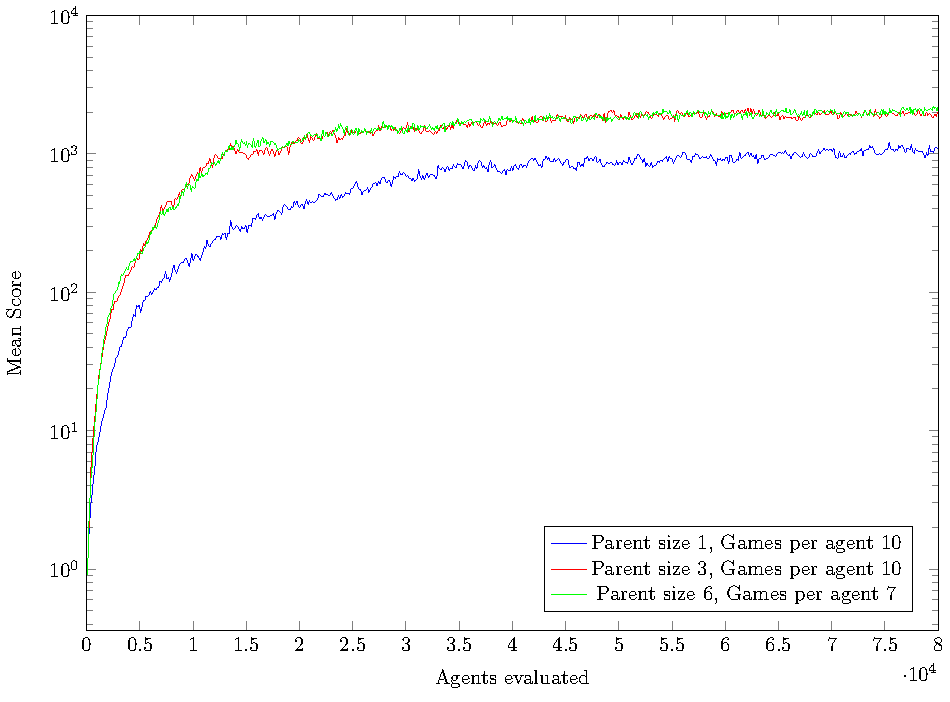
\includegraphics[scale=1]{data/ce_population_offspring/bestofeach_population/13x/PlotFile.pdf}
\caption{Best performing configurations for population size 13}
\end{figure}

\clearpage

\begin{table}[H]
\centering
\small
\begin{tabular}{c c c r r r r}
Population & Parent & Games per Agent & mean & Q1 & Q2 & Q3\\
\hline
$22$ & $2$ & 7 & $1843.644$ & $1575.732$ & $1860.815$ & $2112.678$\\
$22$ & $5$ & 5 & $2371.793$ & $2013.168$ & $2412.815$ & $2708.931$\\
$22$ & $11$ & 7 & $2463.227$ & $2091.090$ & $2384.230$ & $2702.740$\\
\end{tabular}
\caption{population 22 - Cross Entropy}
\end{table}

\begin{figure}[H]
\centering
\includegraphics[scale=1]{data/ce_population_offspring/bestofeach_population/22x/PlotFile.pdf}
\caption{Best performing configurations for population size 22}
\end{figure}

\clearpage

\begin{table}[H]
\centering
\small
\begin{tabular}{c c c r r r r}
Population & Parent & Games per Agent & mean & Q1 & Q2 & Q3\\
\hline
$50$ & $5$ & 3 & $2524.279$ & $2195.189$ & $2501.985$ & $2848.859$\\
$50$ & $12$ & 5 & $2749.991$ & $2605.171$ & $2702.400$ & $2835.960$\\
$50$ & $25$ & 3 & $2572.860$ & $2308.748$ & $2615.185$ & $2861.858$\\
\end{tabular}
\caption{population 50 - Cross Entropy}
\end{table}

\begin{figure}[H]
\centering
\includegraphics[scale=1]{data/ce_population_offspring/bestofeach_population/50x/PlotFile.pdf}
\caption{Best performing configurations for population size 50}
\end{figure}

\clearpage

\begin{table}[H]
\centering
\small
\begin{tabular}{c c c r r r r}
Population & Parent & Games per Agent & mean & Q1 & Q2 & Q3\\
\hline
$100$ & $10$ & 10 & $2880.385$ & $2636.640$ & $2828.880$ & $3108.429$\\
$100$ & $25$ & 3 & $2776.560$ & $2397.691$ & $2742.950$ & $3027.541$\\
$100$ & $50$ & 3 & $2622.402$ & $2318.410$ & $2714.500$ & $2905.521$\\
\end{tabular}
\caption{population 100 - Cross Entropy}
\end{table}

\begin{figure}[H]
\centering
\includegraphics[scale=1]{data/ce_population_offspring/bestofeach_population/100x/PlotFile.pdf}
\caption{Best performing configurations for population size 100}
\end{figure}

\clearpage

\begin{table}[H]
\centering
\small
\begin{tabular}{c c c r r r r}
Population & Parent & Games per Agent & mean & Q1 & Q2 & Q3\\
\hline
$200$ & $20$ & 1 & $2880.572$ & $2596.999$ & $2764.400$ & $3184.290$\\
$200$ & $50$ & 1 & $2950.767$ & $2564.118$ & $2841.065$ & $3377.189$\\
$200$ & $100$ & 1 & $2589.020$ & $2391.080$ & $2594.285$ & $2798.470$\\
\end{tabular}
\caption{population 200 - Cross Entropy}
\end{table}

\begin{figure}[H]
\centering
\includegraphics[scale=1]{data/ce_population_offspring/bestofeach_population/200x/PlotFile.pdf}
\caption{Best performing configurations for population size 200}
\end{figure}

\clearpage

\begin{table}[H]
\centering
\small
\begin{tabular}{c c c r r r r}
Population & Parent & Games per Agent & mean & Q1 & Q2 & Q3\\
\hline
$13$ & $6$ & 7 & $2173.595$ & $1818.110$ & $2105.500$ & $2398.201$\\
$22$ & $5$ & 5 & $2371.793$ & $2013.168$ & $2412.815$ & $2708.931$\\
$50$ & $12$ & 5 & $2749.991$ & $2605.171$ & $2702.400$ & $2835.960$\\
$100$ & $25$ & 3 & $2776.560$ & $2397.691$ & $2742.950$ & $3027.541$\\
$200$ & $50$ & 1 & $2950.767$ & $2564.118$ & $2841.065$ & $3377.189$\\
\end{tabular}
\caption{Best configurations of all population sizes - Cross Entropy}
\end{table}

\begin{figure}[H]
\centering
\includegraphics[scale=1]{data/ce_population_offspring/bestofall_population/PlotFile.pdf}
\caption{Best configurations of all population sizes - Cross Entropy}
\end{figure}

% initial sigma cma experiment
\clearpage

\subsection{Optimal settings for CMA - Initial Step-size \label{appendixCMAInitialSigma}}
Experiments to find the best initial step-size for CMA.

\begin{table}[h]
\centering
\caption{Overview of the two table formats}
\begin{tabular}{l r}
Optimizer & CMA\\
Number of Evaluations & 8000\\
Number of Learning Games &30\\
Population size& 13\\
Parent size & 6\\
Games per Agent & 1\\
Tetris Type & Normal\\
\hline
Recombination Type & Superlinear\\
Initial Sigma & See table \ref{InitialSigmaTest}
\end{tabular}
\end{table}

with the following initial sigma

\begin{table}[H]
\centering
\begin{tabular}{c | c c c c c c}
$\sigma_0$ & 0.1 & 0.2 & 0.5 & 0.8 & 1.0
\end{tabular}
\caption{Initial sigma configurations \label{InitialSigmaTest}}
\end{table}
This sections lists the raw graphs of the experiments that were
to determine the effect of the initial sigma setting. 

\begin{tabular}{@{}l@{}l@{}}
\includegraphics[scale=1]{plots/cma_initial_sigma_0_1} &
\includegraphics[scale=1]{plots/cma_initial_sigma_0_2}
\end{tabular}

\begin{tabular}{@{}l@{}l@{}}
\includegraphics[scale=1]{plots/cma_initial_sigma_0_5} &
\includegraphics[scale=1]{plots/cma_initial_sigma_0_8}
\end{tabular}

\begin{tabular}{@{}l@{}l@{}}
\includegraphics[scale=1]{plots/cma_initial_sigma_1_0} &
\end{tabular}



\begin{figure}[H]
\centering
\begin{tabular}{r | r r r r r}
$\sigma_0$ & mean & Q1 & Q2 & Q3\\
\hline
0.1 & 50769.3 & 21301.1 & 54588.7 & 73972.4\\
0.2 & 42290.6 & 32180.2 & 42290.6 & 49337.4\\
0.5 & 53893.7 & 14211.1 & 66773.0 & 85816.7\\
0.8 & 37557.7 & 1422.8  & 15450.8 & 93719.4\\
1.0 & 49537.9 & 31369.8 & 49537.4 & 58454.6
\end{tabular}
\caption{Results of CMA-ES with adjusted initial step-size \label{CMAInitialSigmaConfigTestAppendix}}
\end{figure}


% initial Lower bound
\clearpage

\subsection{Optimal settings for CMA - Lower bound \label{appendixCMALowerBound}}
\comment{Lower boud plots are wrong}\\
Experiments to find the best lower bound of $\sigma \lambda_n > l$ for CMA.

\begin{table}[h]
\centering
\caption{Overview of the two table formats}
\begin{tabular}{l r}
Optimizer & CMA\\
Number of Evaluations & 8000\\
Number of Learning Games &30\\
Population size& 13\\
Parent size & 6\\
Games per Agent & 1\\
Tetris Type & Normal\\
\hline
Recombination Type & Superlinear\\
Lower bound & See table \ref{appendixLowerBound}
\end{tabular}
\end{table}

with the following lower bounds

\begin{table}[H]
\centering
\begin{tabular}{c | c c c}
$l$ & 0.5 & 2.0 & 4.0
\end{tabular}
\caption{Lower bound configurations \label{appendixLowerBound}}
\end{table}
This sections lists the raw graphs of the experiments that were
to determine the effect of the initial sigma setting. 

\begin{tabular}{@{}l@{}l@{}}
\includegraphics[scale=1]{plots/cma_lower_bound_0_5} &
\includegraphics[scale=1]{plots/cma_lower_bound_2_0}\\
\includegraphics[scale=1]{plots/cma_lower_bound_4_0} &
\end{tabular}

\begin{figure}[H]
\centering
\begin{tabular}{r | r r r r r}
$l$ & mean & Q1 & Q2 & Q3\\
\hline
0.5 & 42800.7 & 6780.8  & 36863.0 & 74722.5\\
2.0 & 80733.4 & 62357.4 & 84349.0 & 108007.5\\
4.0 & 61497.2 & 55621.7 & 64940.1 & 81991.6\\
\end{tabular}
\caption{Results of CMA-ES lower bounds \label{appendixCMALowerBoundConfigTest}}
\end{figure}





\clearpage

\subsection{Optimal settings for CMA - Experiment for finding the optimal settings \label{appendixCMAPopulationParent}}
Experiments finding the best configuration of population and parent size with recombination type. The parent size is dependent on the recombination type, therefore we tested these parameter together.
\begin{table}[h]
\centering
\begin{tabular}{l r}
Optimizer & CMA\\
Number of Evaluations & 80000\\
Number of Learning Games &30\\
Population size& See table \ref{SuperCMAExperiment}\\
Parent size & See table \ref{SuperCMAExperiment}\\
Games per Agent & See table \ref{SuperCMAExperiment}\\
Tetris Type & Hard\\
\hline
Recombination Type & See table \ref{SuperCMAExperiment}\\
Initial Sigma & 1
\end{tabular}
\caption{CMA experiment parameters for testing games per agent}
\end{table}

\begin{table}[H]
\centering
\begin{tabular}{c c l c}
Population Size & Parent size & Recombination Type & Games per Agent\\
\hline
$12$ & $1$ & EQUAL/LINEAR/SUPERLINEAR & 1/3/5/7/10\\
$12$ & $3$ & EQUAL & 1/3/5/7/10\\
$12$ & $6$ & LINEAR/SUPERLINEAR & 1/3/5/7/10\\
$22$ & $2$ & EQUAL/LINEAR/SUPERLINEAR & 1/3/5/7/10\\
$22$ & $5$ & EQUAL & 1/3/5/7/10\\
$22$ & $11$ & LINEAR/SUPERLINEAR & 1/3/5/7/10\\
$50$ & $5$ & EQUAL/LINEAR/SUPERLINEAR & 1/3/5/7/10\\
$50$ & $12$ & EQUAL & 1/3/5/7/10\\
$50$ & $25$ & LINEAR/SUPERLINEAR & 1/3/5/7/10\\
$100$ & $10$ & EQUAL/LINEAR/SUPERLINEAR & 1/3/5/7/10\\
$100$ & $25$ & EQUAL & 1/3/5/7/10\\
$100$ & $50$ & LINEAR/SUPERLINEAR & 1/3/5/7/10
\end{tabular}
\caption{Full experiments overview \label{SuperCMAExperimentAppendix}}
\end{table}


%\begin{figure}
%\centering
%\caption{Population size 12, Parent size 1, \\Meanscore of EQUAL recombination}
%\includegraphics[scale=0.5]{data/cma_population_offspring/12x_split/equal_l12_o1/mean/PlotFile.pdf}
%\end{figure}


\clearpage

\begin{figure}
	\centering
	\captionsetup[subfigure]{justification=centering}
    \begin{subfigure}[b]{0.49\textwidth}
    	\caption{Population size 12, Parent size 1,\\EQUAL recombination}
        \includegraphics[width=\textwidth]{data/cma_population_offspring/12x_split/equal_l12_o1/mean/PlotFile.pdf}
    \end{subfigure} 
    \begin{subfigure}[b]{0.49\textwidth}
    	\caption{Population size 12, Parent size 3,\\EQUAL recombination}
        \includegraphics[width=\textwidth]{data/cma_population_offspring/12x_split/equal_l12_o3/mean/PlotFile.pdf}
    \end{subfigure}
    \begin{subfigure}[b]{0.49\textwidth}
    	\caption{Population size 12, Parent size 1,\\LINEAR recombination}
        \includegraphics[width=\textwidth]{data/cma_population_offspring/12x_split/linear_l12_o1/mean/PlotFile.pdf}
    \end{subfigure}
    \begin{subfigure}[b]{0.49\textwidth}
    	\caption{Population size 12, Parent size 6,\\LINEAR recombination}
        \includegraphics[width=\textwidth]{data/cma_population_offspring/12x_split/linear_l12_o6/mean/PlotFile.pdf}
    \end{subfigure}
    \begin{subfigure}[b]{0.49\textwidth}
    	\caption{Population size 12, Parent size 1,\\SUPERLINEAR recombination}
        \includegraphics[width=\textwidth]{data/cma_population_offspring/12x_split/superlinear_l12_o1/mean/PlotFile.pdf}
    \end{subfigure}
    \begin{subfigure}[b]{0.49\textwidth}
    	\caption{Population size 12, Parent size 6,\\SUPERLINEAR recombination}
        \includegraphics[width=\textwidth]{data/cma_population_offspring/12x_split/superlinear_l12_o6/mean/PlotFile.pdf}
    \end{subfigure}
    
    \caption{Mean results for population size 12 with variating recombination}
\end{figure}

\begin{figure}
    \centering
    \captionsetup[subfigure]{justification=centering}
    \begin{subfigure}[b]{0.49\textwidth}
    	\centering
        \caption{Population size 22, Parent size 2,\\EQUAL recombination}
        \includegraphics[width=\textwidth]{data/cma_population_offspring/22x_split/equal_l22_o2/mean/PlotFile.pdf}
    \end{subfigure} 
    \begin{subfigure}[b]{0.49\textwidth}
    	\centering
    	\caption{Population size 22, Parent size 5,\\EQUAL recombination}
        \includegraphics[width=\textwidth]{data/cma_population_offspring/22x_split/equal_l22_o5/mean/PlotFile.pdf}
    \end{subfigure}
    \begin{subfigure}[b]{0.49\textwidth}
    	\centering
    	\caption{Population size 22, Parent size 2,\\LINEAR recombination}
        \includegraphics[width=\textwidth]{data/cma_population_offspring/22x_split/linear_l22_o2/mean/PlotFile.pdf}
    \end{subfigure}
    \begin{subfigure}[b]{0.49\textwidth}
    	\centering
    	\caption{Population size 22, Parent size 11,\\LINEAR recombination}
        \includegraphics[width=\textwidth]{data/cma_population_offspring/22x_split/linear_l22_o11/mean/PlotFile.pdf}
    \end{subfigure}
    \begin{subfigure}[b]{0.49\textwidth}
    	\centering
    	\caption{Population size 22, Parent size 2,\\SUPERLINEAR recombination}
        \includegraphics[width=\textwidth]{data/cma_population_offspring/22x_split/superlinear_l22_o2/mean/PlotFile.pdf}
    \end{subfigure}
    \begin{subfigure}[b]{0.49\textwidth}
    	\centering
    	\caption{Population size 22, Parent size 11,\\SUPERLINEAR recombination}
        \includegraphics[width=\textwidth]{data/cma_population_offspring/22x_split/superlinear_l22_o11/mean/PlotFile.pdf}
    \end{subfigure}
    
    \caption{Mean results for population size 22 with variating recombination}
\end{figure}

\begin{figure}
    \centering
    \captionsetup[subfigure]{justification=centering}
    \begin{subfigure}[b]{0.49\textwidth}
    	\centering
        \caption{Population size 50, Parent size 5,\\EQUAL recombination}
        \includegraphics[width=\textwidth]{data/cma_population_offspring/50x_split/equal_l50_o5/mean/PlotFile.pdf}
    \end{subfigure} 
    \begin{subfigure}[b]{0.49\textwidth}
    	\centering
    	\caption{Population size 50, Parent size 12,\\EQUAL recombination}
        \includegraphics[width=\textwidth]{data/cma_population_offspring/50x_split/equal_l50_o12/mean/PlotFile.pdf}
    \end{subfigure}
    \begin{subfigure}[b]{0.49\textwidth}
    	\centering
    	\caption{Population size 50, Parent size 5,\\LINEAR recombination}
        \includegraphics[width=\textwidth]{data/cma_population_offspring/50x_split/linear_l50_o5/mean/PlotFile.pdf}
    \end{subfigure}
    \begin{subfigure}[b]{0.49\textwidth}
    	\centering
    	\caption{Population size 50, Parent size 25,\\LINEAR recombination}
        \includegraphics[width=\textwidth]{data/cma_population_offspring/50x_split/linear_l50_o25/mean/PlotFile.pdf}
    \end{subfigure}
    \begin{subfigure}[b]{0.49\textwidth}
    	\centering
    	\caption{Population size 50, Parent size 5,\\SUPERLINEAR recombination}
        \includegraphics[width=\textwidth]{data/cma_population_offspring/50x_split/superlinear_l50_o5/mean/PlotFile.pdf}
    \end{subfigure}
    \begin{subfigure}[b]{0.49\textwidth}
    	\centering
    	\caption{Population size 50, Parent size 25,\\SUPERLINEAR recombination}
        \includegraphics[width=\textwidth]{data/cma_population_offspring/50x_split/superlinear_l50_o25/mean/PlotFile.pdf}
    \end{subfigure}
    
    \caption{Mean results for population size 50 with variating recombination}
\end{figure}

\begin{figure}
    \centering
    \captionsetup[subfigure]{justification=centering}
    \begin{subfigure}[b]{0.49\textwidth}
    	\centering
        \caption{Population size 100, Parent size 10,\\EQUAL recombination}
        \includegraphics[width=\textwidth]{data/cma_population_offspring/100x_split/equal_l100_o10/mean/PlotFile.pdf}
    \end{subfigure} 
    \begin{subfigure}[b]{0.49\textwidth}
    	\centering
    	\caption{Population size 100, Parent size 25,\\EQUAL recombination}
        \includegraphics[width=\textwidth]{data/cma_population_offspring/100x_split/equal_l100_o25/mean/PlotFile.pdf}
    \end{subfigure}
    \begin{subfigure}[b]{0.49\textwidth}
    	\centering
    	\caption{Population size 100, Parent size 10,\\LINEAR recombination}
        \includegraphics[width=\textwidth]{data/cma_population_offspring/100x_split/linear_l100_o10/mean/PlotFile.pdf}
    \end{subfigure}
    \begin{subfigure}[b]{0.49\textwidth}
    	\centering
    	\caption{Population size 100, Parent size 50,\\LINEAR recombination}
        \includegraphics[width=\textwidth]{data/cma_population_offspring/100x_split/linear_l100_o50/mean/PlotFile.pdf}
    \end{subfigure}
    \begin{subfigure}[b]{0.49\textwidth}
    	\centering
    	\caption{Population size 100, Parent size 10,\\SUPERLINEAR recombination}
        \includegraphics[width=\textwidth]{data/cma_population_offspring/100x_split/superlinear_l100_o10/mean/PlotFile.pdf}
    \end{subfigure}
    \begin{subfigure}[b]{0.49\textwidth}
    	\centering
    	\caption{Population size 100, Parent size 50,\\SUPERLINEAR recombination}
        \includegraphics[width=\textwidth]{data/cma_population_offspring/100x_split/superlinear_l100_o50/mean/PlotFile.pdf}
    \end{subfigure}
    
    \caption{Mean results for population size 100 with variating recombination}
\end{figure}

\clearpage

\begin{table}[H]
\centering
\small
\begin{tabular}{c c c c r r r r}
Population & Parent & Recombination & Games per Agent & mean & Q1 & Q2 & Q3\\
\hline
$12$ & $1$ & EQUAL & 1 & $86.998$ & $53.557$ & $63.417$ & $111.313$\\
$12$ & $1$ & EQUAL & 3 & $458.616$ & $256.637$ & $349.033$ & $576.899$\\
$12$ & $1$ & EQUAL & 5 & $1089.245$ & $850.220$ & $1104.535$ & $1299.039$\\
$12$ & $1$ & EQUAL & 7 & $1081.248$ & $918.049$ & $1089.400$ & $1248.619$\\
\hdashline
$12$ & $1$ & EQUAL & 10 & $1134.339$ & $863.523$ & $1061.050$ & $1297.359$\\
\hdashline
$12$ & $1$ & LINEAR & 1 & $76.228$ & $45.587$ & $53.917$ & $74.353$\\
$12$ & $1$ & LINEAR & 3 & $717.883$ & $380.890$ & $556.950$ & $878.597$\\
$12$ & $1$ & LINEAR & 5 & $720.393$ & $503.130$ & $708.484$ & $893.517$\\
$12$ & $1$ & LINEAR & 7 & $1043.547$ & $732.367$ & $969.217$ & $1234.040$\\
\hdashline
$12$ & $1$ & LINEAR & 10 & $1276.041$ & $1135.609$ & $1196.120$ & $1502.029$\\
\hdashline
$12$ & $1$ & SUPERLINEAR & 1 & $64.211$ & $45.687$ & $64.483$ & $78.090$\\
$12$ & $1$ & SUPERLINEAR & 3 & $646.760$ & $429.043$ & $661.817$ & $860.470$\\
$12$ & $1$ & SUPERLINEAR & 5 & $925.410$ & $726.360$ & $948.300$ & $1158.021$\\
$12$ & $1$ & SUPERLINEAR & 7 & $1034.002$ & $792.567$ & $924.350$ & $1269.131$\\
\hdashline
$12$ & $1$ & SUPERLINEAR & 10 & $1401.300$ & $1194.430$ & $1440.500$ & $1569.012$\\
\hdashline
\end{tabular}
\caption{Population size 12, Parent size 1 - "Cross Entropy"-inspired configuration}
\end{table}

\begin{table}[H]
\centering
\small
\begin{tabular}{c c c c r r r r}
Population & Parent & Recombination & Games per Agent & mean & Q1 & Q2 & Q3\\
\hline
$12$ & $3$ & EQUAL & 1 & $461.762$ & $266.047$ & $408.034$ & $639.013$\\
$12$ & $3$ & EQUAL & 3 & $1364.176$ & $1199.310$ & $1438.880$ & $1579.560$\\
$12$ & $3$ & EQUAL & 5 & $1754.634$ & $1464.239$ & $1621.035$ & $1945.010$\\
$12$ & $3$ & EQUAL & 7 & $1884.765$ & $1614.661$ & $1800.485$ & $2156.972$\\
\hdashline
$12$ & $3$ & EQUAL & 10 & $1940.783$ & $1566.721$ & $1913.415$ & $2210.251$\\
\hdashline
$12$ & $6$ & LINEAR & 1 & $626.867$ & $447.440$ & $538.150$ & $724.913$\\
$12$ & $6$ & LINEAR & 3 & $1844.453$ & $1568.829$ & $1831.265$ & $2227.479$\\
$12$ & $6$ & LINEAR & 5 & $2148.853$ & $1846.459$ & $2118.335$ & $2588.010$\\
$12$ & $6$ & LINEAR & 7 & $2144.345$ & $1860.340$ & $2160.900$ & $2428.348$\\
\hdashline
$12$ & $6$ & LINEAR & 10 & $2365.089$ & $2072.719$ & $2263.665$ & $2637.732$\\
\hdashline
$12$ & $6$ & SUPERLINEAR & 1 & $669.005$ & $506.817$ & $648.167$ & $836.377$\\
$12$ & $6$ & SUPERLINEAR & 3 & $1901.814$ & $1572.260$ & $1932.515$ & $2151.189$\\
$12$ & $6$ & SUPERLINEAR & 5 & $2098.654$ & $1965.472$ & $2115.250$ & $2453.069$\\
$12$ & $6$ & SUPERLINEAR & 7 & $2402.888$ & $2055.329$ & $2387.700$ & $2635.870$\\
\hdashline
$12$ & $6$ & SUPERLINEAR & 10 & $2472.293$ & $2194.049$ & $2430.780$ & $2709.040$\\
\hdashline
\end{tabular}
\caption{Population size 12, Parent size 3/6 - CMA configuration}
\end{table}


\begin{table}[H]
\centering
\small
\begin{tabular}{c c c c r r r r}
Population & Parent & Recombination & Games per Agent & mean & Q1 & Q2 & Q3\\
\hline
$22$ & $2$ & EQUAL & 1 & $684.551$ & $429.890$ & $597.534$ & $877.150$\\
$22$ & $2$ & EQUAL & 3 & $1473.504$ & $1197.290$ & $1490.865$ & $1713.091$\\
$22$ & $2$ & EQUAL & 5 & $1648.777$ & $1425.150$ & $1630.535$ & $1826.372$\\
$22$ & $2$ & EQUAL & 7 & $1762.786$ & $1521.832$ & $1769.180$ & $2033.799$\\
\hdashline
$22$ & $2$ & EQUAL & 10 & $1895.305$ & $1630.891$ & $1849.75$ & $2043.442$\\
\hdashline
$22$ & $2$ & LINEAR & 1 & $513.271$ & $398.023$ & $524.850$ & $589.467$\\
$22$ & $2$ & LINEAR & 3 & $1374.423$ & $1082.859$ & $1255.985$ & $1561.119$\\
$22$ & $2$ & LINEAR & 5 & $1607.568$ & $1513.389$ & $1656.465$ & $1791.069$\\
$22$ & $2$ & LINEAR & 7 & $1770.294$ & $1538.900$ & $1691.165$ & $1881.590$\\
\hdashline
$22$ & $2$ & LINEAR & 10 & $2158.396$ & $1966.351$ & $2085.235$ & $2162.541$\\
\hdashline
$22$ & $2$ & SUPERLINEAR & 1 & $698.811$ & $359.367$ & $622.467$ & $937.423$\\
$22$ & $2$ & SUPERLINEAR & 3 & $1447.704$ & $1281.119$ & $1452.680$ & $1640.468$\\
$22$ & $2$ & SUPERLINEAR & 5 & $1714.875$ & $1362.931$ & $1733.230$ & $2023.590$\\
\hdashline
$22$ & $2$ & SUPERLINEAR & 7 & $1783.623$ & $1603.389$ & $1720.335$ & $1937.749$\\
\hdashline
$22$ & $2$ & SUPERLINEAR & 10 & $1859.642$ & $1636.870$ & $1915.650$ & $2208.830$\\
\end{tabular}
\caption{Population size 22, Parent size 2 - "Cross Entropy"-inspired configuration}
\end{table}


\begin{table}[H]
\centering
\small
\begin{tabular}{c c c c r r r r}
Population & Parent & Recombination & Games per Agent & mean & Q1 & Q2 & Q3\\
\hline
$22$ & $5$ & EQUAL & 1 & $1411.458$ & $1207.060$ & $1528.050$ & $1707.590$\\
$22$ & $5$ & EQUAL & 3 & $2209.730$ & $2129.521$ & $2213.285$ & $2471.751$\\
$22$ & $5$ & EQUAL & 5 & $2274.419$ & $1933.249$ & $2187.800$ & $2570.399$\\
$22$ & $5$ & EQUAL & 7 & $2386.088$ & $2112.841$ & $2328.500$ & $2573.261$\\
\hdashline
$22$ & $5$ & EQUAL & 10 & $2462.409$ & $2277.180$ & $2418.100$ & $2600.411$\\
\hdashline
$22$ & $11$ & LINEAR & 1 & $1604.434$ & $1181.603$ & $1549.735$ & $1678.111$\\
$22$ & $11$ & LINEAR & 3 & $2774.378$ & $2460.992$ & $2594.900$ & $3030.310$\\
$22$ & $11$ & LINEAR & 5 & $2530.796$ & $2382.050$ & $2658.915$ & $2990.851$\\
\hdashline
$22$ & $11$ & LINEAR & 7 & $2763.353$ & $2597.450$ & $2705.080$ & $3000.242$\\
\hdashline
$22$ & $11$ & LINEAR & 10 & $2707.983$ & $2146.209$ & $2800.435$ & $3273.401$\\
$22$ & $11$ & SUPERLINEAR & 1 & $1666.214$ & $1447.430$ & $1660.900$ & $1856.908$\\
$22$ & $11$ & SUPERLINEAR & 3 & $2581.119$ & $2306.02$ & $2548.380$ & $2759.428$\\
$22$ & $11$ & SUPERLINEAR & 5 & $2635.429$ & $2409.620$ & $2574.785$ & $2863.849$\\
$22$ & $11$ & SUPERLINEAR & 7 & $2661.638$ & $2411.232$ & $2575.030$ & $2945.200$\\
\hdashline
$22$ & $11$ & SUPERLINEAR & 10 & $2849.220$ & $2500.231$ & $2835.450$ & $3143.121$\\
\hdashline
\end{tabular}
\caption{Population size 22, Parent size 5/11 - CMA configuration}
\end{table}


\begin{table}[H]
\centering
\small
\begin{tabular}{c c c c r r r r}
Population & Parent & Recombination & Games per Agent & mean & Q1 & Q2 & Q3\\
\hline
$50$ & $5$ & EQUAL & 1 & $1999.620$ & $1789.150$ & $1902.020$ & $2161.948$\\
$50$ & $5$ & EQUAL & 3 & $2471.173$ & $2178.651$ & $2389.070$ & $2660.220$\\
$50$ & $5$ & EQUAL & 5 & $2849.482$ & $2459.460$ & $2875.835$ & $3276.190$\\
$50$ & $5$ & EQUAL & 7 & $2466.801$ & $2355.349$ & $2517.335$ & $2644.751$\\
\hdashline
$50$ & $5$ & EQUAL & 10 & $2801.923$ & $2479.088$ & $2915.980$ & $3081.018$\\
\hdashline
$50$ & $5$ & LINEAR & 1 & $1931.703$ & $1659.412$ & $1885.150$ & $2130.479$\\
$50$ & $5$ & LINEAR & 3 & $2612.345$ & $2380.759$ & $2529.150$ & $2796.729$\\
$50$ & $5$ & LINEAR & 5 & $2410.633$ & $2067.111$ & $2357.830$ & $2675.572$\\
\hdashline
$50$ & $5$ & LINEAR & 7 & $2842.090$ & $2497.952$ & $2922.965$ & $3136.509$\\
\hdashline
$50$ & $5$ & LINEAR & 10 & $2696.952$ & $2518.290$ & $2678.400$ & $2923.010$\\
$50$ & $5$ & SUPERLINEAR & 1 & $1962.410$ & $1715.568$ & $1781.865$ & $2009.488$\\
$50$ & $5$ & SUPERLINEAR & 3 & $2493.884$ & $2220.200$ & $2398.230$ & $2762.609$\\
$50$ & $5$ & SUPERLINEAR & 5 & $2541.065$ & $2268.881$ & $2593.150$ & $2974.558$\\
$50$ & $5$ & SUPERLINEAR & 7 & $2647.412$ & $2448.010$ & $2745.400$ & $3058.870$\\
\hdashline
$50$ & $5$ & SUPERLINEAR & 10 & $2757.388$ & $2357.062$ & $2886.950$ & $3187.282$\\
\hdashline
\end{tabular}
\caption{Population size 50, Parent size 5 - "Cross Entropy"-inspired configuration}
\end{table}

\begin{table}[H]
\centering
\small
\begin{tabular}{c c c c r r r r}
Population & Parent & Recombination & Games per Agent & mean & Q1 & Q2 & Q3\\
\hline
$50$ & $12$ & EQUAL & 1 & $2395.091$ & $2095.030$ & $2442.485$ & $2778.160$\\
$50$ & $12$ & EQUAL & 3 & $2878.667$ & $2550.399$ & $2794.915$ & $3102.639$\\
$50$ & $12$ & EQUAL & 5 & $2760.846$ & $2509.000$ & $2695.450$ & $3006.988$\\
$50$ & $12$ & EQUAL & 7 & $2913.846$ & $2627.310$ & $2809.600$ & $3128.439$\\
\hdashline
$50$ & $12$ & EQUAL & 10 & $2957.794$ & $2636.478$ & $2843.380$ & $3222.420$\\
\hdashline
$50$ & $25$ & LINEAR & 1 & $2355.564$ & $2262.991$ & $2543.665$ & $2752.431$\\
$50$ & $25$ & LINEAR & 3 & $2857.170$ & $2464.251$ & $2830.765$ & $3209.929$\\
$50$ & $25$ & LINEAR & 5 & $3036.881$ & $2807.050$ & $3095.300$ & $3416.750$\\
$50$ & $25$ & LINEAR & 7 & $3043.399$ & $2821.049$ & $3099.235$ & $3239.032$\\
\hdashline
$50$ & $25$ & LINEAR & 10 & $3167.873$ & $2941.590$ & $3130.385$ & $3415.520$\\
\hdashline
$50$ & $25$ & SUPERLINEAR & 1 & $2418.057$ & $2352.851$ & $2553.465$ & $2718.759$\\
$50$ & $25$ & SUPERLINEAR & 3 & $2958.686$ & $2715.579$ & $2941.800$ & $3173.361$\\
\hdashline
$50$ & $25$ & SUPERLINEAR & 5 & $3211.658$ & $2889.689$ & $3305.485$ & $3694.480$\\
\hdashline
$50$ & $25$ & SUPERLINEAR & 7 & $3147.611$ & $2799.510$ & $3123.550$ & $3457.999$\\
$50$ & $25$ & SUPERLINEAR & 10 & $3265.516$ & $2928.771$ & $3162.250$ & $3389.121$\\
\end{tabular}
\caption{Population size 50, Parent size 12/25 - CMA configuration}
\end{table}


\begin{table}[H]
\centering
\small
\begin{tabular}{c c c c r r r r}
Population & Parent & Recombination & Games per Agent & mean & Q1 & Q2 & Q3\\
\hline
$100$ & $10$ & EQUAL & 1 & $2528.158$ & $2380.122$ & $2680.785$ & $2782.850$\\
$100$ & $10$ & EQUAL & 3 & $2763.118$ & $2488.878$ & $2696.685$ & $2962.190$\\
$100$ & $10$ & EQUAL & 5 & $2783.246$ & $2399.949$ & $2693.285$ & $2900.391$\\
\hdashline
$100$ & $10$ & EQUAL & 7 & $3016.342$ & $2835.049$ & $2985.150$ & $3292.910$\\
\hdashline
$100$ & $10$ & EQUAL & 10 & $2940.037$ & $2703.859$ & $2920.615$ & $3216.410$\\
$100$ & $10$ & LINEAR & 1 & $2655.099$ & $2409.162$ & $2691.850$ & $2961.091$\\
$100$ & $10$ & LINEAR & 3 & $2823.674$ & $2526.560$ & $2792.500$ & $2974.549$\\
\hdashline
$100$ & $10$ & LINEAR & 5 & $3204.395$ & $2928.050$ & $3248.515$ & $3371.008$\\
\hdashline
$100$ & $10$ & LINEAR & 7 & $2993.126$ & $2639.021$ & $3031.065$ & $3277.642$\\
$100$ & $10$ & LINEAR & 10 & $2726.273$ & $2402.502$ & $2748.535$ & $3009.198$\\
$100$ & $10$ & SUPERLINEAR & 1 & $2571.936$ & $2211.051$ & $2634.850$ & $2811.190$\\
$100$ & $10$ & SUPERLINEAR & 3 & $2853.959$ & $2552.749$ & $2870.600$ & $3005.292$\\
\hdashline
$100$ & $10$ & SUPERLINEAR & 5 & $3009.495$ & $2816.660$ & $2989.900$ & $3189.310$\\
\hdashline
$100$ & $10$ & SUPERLINEAR & 7 & $2935.614$ & $2540.342$ & $2887.085$ & $3232.508$\\
$100$ & $10$ & SUPERLINEAR & 10 & $2941.535$ & $2705.290$ & $2893.580$ & $3153.510$\\
\end{tabular}
\caption{Population size 100, Parent size 10 - "Cross Entropy"-inspired configuration}
\end{table}


\begin{table}[H]
\centering
\small
\begin{tabular}{c c c c r r r r}
Population & Parent & Recombination & Games per Agent & mean & Q1 & Q2 & Q3\\
\hline
$100$ & $25$ & EQUAL & 1 & $2885.131$ & $2565.572$ & $2886.735$ & $3231.600$\\
\hdashline
$100$ & $25$ & EQUAL & 3 & $3244.544$ & $2924.488$ & $3270.885$ & $3525.671$\\
\hdashline
$100$ & $25$ & EQUAL & 5 & $3065.143$ & $2773.848$ & $3032.830$ & $3347.358$\\
$100$ & $25$ & EQUAL & 7 & $3125.085$ & $2758.298$ & $3054.950$ & $3486.672$\\
$100$ & $25$ & EQUAL & 10 & $3258.533$ & $2976.271$ & $3144.750$ & $3598.868$\\
$100$ & $50$ & LINEAR & 1 & $3099.651$ & $2814.781$ & $3019.830$ & $3466.380$\\
$100$ & $50$ & LINEAR & 3 & $3125.019$ & $2706.618$ & $3087.815$ & $3368.681$\\
$100$ & $50$ & LINEAR & 5 & $3171.761$ & $2941.030$ & $3138.515$ & $3436.670$\\
\hdashline
$100$ & $50$ & LINEAR & 7 & $3322.076$ & $3160.098$ & $3289.370$ & $3537.850$\\
\hdashline
$100$ & $50$ & LINEAR & 10 & $3320.153$ & $3040.611$ & $3291.335$ & $3633.491$\\
$100$ & $50$ & SUPERLINEAR & 1 & $3162.245$ & $2815.099$ & $3093.050$ & $3482.748$\\
$100$ & $50$ & SUPERLINEAR & 3 & $3188.324$ & $2781.382$ & $3258.400$ & $3413.710$\\
\hdashline
$100$ & $50$ & SUPERLINEAR & 5 & $3304.119$ & $3004.140$ & $3226.235$ & $3679.359$\\
\hdashline
$100$ & $50$ & SUPERLINEAR & 7 & $3072.331$ & $2682.300$ & $2964.850$ & $3403.132$\\
$100$ & $50$ & SUPERLINEAR & 10 & $3106.917$ & $2914.349$ & $3162.250$ & $3324.970$\\
\end{tabular}
\caption{Population size 100, Parent size 25/50 - CMA configuration}
\end{table}

\clearpage

\begin{table}[H]
\centering
\small
\begin{tabular}{c c c c r r r r}
Population & Parent & Recombination & Games per Agent & mean & Q1 & Q2 & Q3\\
\hline
$12$ & $1$ & EQUAL & 10 & $1134.339$ & $863.523$ & $1061.050$ & $1297.359$\\
$12$ & $1$ & LINEAR & 10 & $1276.041$ & $1135.609$ & $1196.120$ & $1502.029$\\
$12$ & $1$ & SUPERLINEAR & 10 & $1401.300$ & $1194.430$ & $1440.500$ & $1569.012$\\
$12$ & $3$ & EQUAL & 10 & $1940.783$ & $1566.721$ & $1913.415$ & $2210.251$\\
$12$ & $6$ & LINEAR & 10 & $2365.089$ & $2072.719$ & $2263.665$ & $2637.732$\\
$12$ & $6$ & SUPERLINEAR & 10 & $2472.293$ & $2194.049$ & $2430.780$ & $2709.040$\\
\end{tabular}
\caption{Best performing configurations for population size 12}
\end{table}

\begin{figure}[H]
\centering
\includegraphics[scale=1]{data/cma_population_offspring/bestofeach_population/12x/PlotFile.pdf}
\caption{Best performing configurations for population size 12}
\end{figure}

\clearpage

\begin{table}[H]
\centering
\small
\begin{tabular}{c c c c r r r r}
Population & Parent & Recombination & Games per Agent & mean & Q1 & Q2 & Q3\\
\hline
$22$ & $2$ & EQUAL & 10 & $1895.305$ & $1630.891$ & $1849.75$ & $2043.442$\\
$22$ & $2$ & LINEAR & 10 & $2158.396$ & $1966.351$ & $2085.235$ & $2162.541$\\
$22$ & $2$ & SUPERLINEAR & 7 & $1783.623$ & $1603.389$ & $1720.335$ & $1937.749$\\
$22$ & $5$ & EQUAL & 10 & $2462.409$ & $2277.180$ & $2418.100$ & $2600.411$\\
$22$ & $11$ & LINEAR & 7 & $2763.353$ & $2597.450$ & $2705.080$ & $3000.242$\\
$22$ & $11$ & SUPERLINEAR & 10 & $2849.220$ & $2500.231$ & $2835.450$ & $3143.121$\\
\end{tabular}
\caption{Best performing configurations for population size 22}
\end{table}

\begin{figure}[H]
\centering
\includegraphics[scale=1]{data/cma_population_offspring/bestofeach_population/22x/PlotFile.pdf}
\caption{Best performing configurations for population size 22}
\end{figure}

\clearpage

\begin{table}[H]
\centering
\small
\begin{tabular}{c c c c r r r r}
Population & Parent & Recombination & Games per Agent & mean & Q1 & Q2 & Q3\\
\hline
$50$ & $5$ & EQUAL & 10 & $2801.923$ & $2479.088$ & $2915.980$ & $3081.018$\\
$50$ & $5$ & LINEAR & 7 & $2842.090$ & $2497.952$ & $2922.965$ & $3136.509$\\
$50$ & $5$ & SUPERLINEAR & 10 & $2757.388$ & $2357.062$ & $2886.950$ & $3187.282$\\
$50$ & $12$ & EQUAL & 10 & $2957.794$ & $2636.478$ & $2843.380$ & $3222.420$\\
$50$ & $25$ & LINEAR & 10 & $3167.873$ & $2941.590$ & $3130.385$ & $3415.520$\\
$50$ & $25$ & SUPERLINEAR & 5 & $3211.658$ & $2889.689$ & $3305.485$ & $3694.480$\\
\end{tabular}
\caption{Best performing configurations for population size 50}
\end{table}

\begin{figure}[H]
\centering
\includegraphics[scale=1]{data/cma_population_offspring/bestofeach_population/50x/PlotFile.pdf}
\caption{Best performing configurations for population size 50}
\end{figure}

\clearpage

\begin{table}[H]
\centering
\small
\begin{tabular}{c c c c r r r r}
Population & Parent & Recombination & Games per Agent & mean & Q1 & Q2 & Q3\\
\hline
$100$ & $10$ & EQUAL & 7 & $3016.342$ & $2835.049$ & $2985.150$ & $3292.910$\\
$100$ & $10$ & LINEAR & 5 & $3204.395$ & $2928.050$ & $3248.515$ & $3371.008$\\
$100$ & $10$ & SUPERLINEAR & 5 & $3009.495$ & $2816.660$ & $2989.900$ & $3189.310$\\
$100$ & $25$ & EQUAL & 3 & $3244.544$ & $2924.488$ & $3270.885$ & $3525.671$\\
$100$ & $50$ & LINEAR & 7 & $3322.076$ & $3160.098$ & $3289.370$ & $3537.850$\\
$100$ & $50$ & SUPERLINEAR & 5 & $3304.119$ & $3004.140$ & $3226.235$ & $3679.359$\\
\end{tabular}
\caption{Best performing configurations for population size 100}
\end{table}

\begin{figure}[H]
\centering
\includegraphics[scale=1]{data/cma_population_offspring/bestofeach_population/100x/PlotFile.pdf}
\caption{Best performing configurations for population size 100}
\end{figure}

\clearpage 

\begin{table}[H]
\centering
\small
\begin{tabular}{c c c c r r r r}
Population & Parent & Recombination & Games per Agent & mean & Q1 & Q2 & Q3\\
\hline
$12$ & $6$ & SUPERLINEAR & 10 & $2472.293$ & $2194.049$ & $2430.780$ & $2709.040$\\
$22$ & $11$ & SUPERLINEAR & 10 & $2849.220$ & $2500.231$ & $2835.450$ & $3143.121$\\
$50$ & $25$ & SUPERLINEAR & 5 & $3211.658$ & $2889.689$ & $3305.485$ & $3694.480$\\
$100$ & $50$ & LINEAR & 7 & $3322.076$ & $3160.098$ & $3289.370$ & $3537.850$\\
\end{tabular}
\caption{Best performing configurations of all population sizes}
\end{table}

\begin{figure}[H]
\centering
\includegraphics[scale=1]{data/cma_population_offspring/bestofall_population/PlotFile.pdf}
\caption{Best performing configurations of all population sizes}
\end{figure}



\clearpage

\subsection{Comparison - Initial comparison}
Comparison between the verified Cross Entropy and Shark (reference to shark) stock setting CMA.

\begin{table}[h]
\centering
\small
\caption{Shark stock CMA and Verified Cross Entropy}
\begin{tabular}{l r}
Optimizer & CMA\\
Number of Evaluations & 8000\\
Number of Learning Games & 30\\
Population size& 13\\
Parent size & 6\\
Games per Agent & 1\\
Tetris Type & Normal\\
\hline
Recombination Type & Superlinear\\
Initial Sigma & 6\\
\quad & \quad
\end{tabular}
\quad
\begin{tabular}{l r}
Optimizer & Cross Entropy\\
Number of Evaluations & 8000\\
Number of Learning Games & 30\\
Population size & 100\\
Parent size & 10\\
Games per Agent & 1\\
Tetris Type & Normal\\
\hline
Sigma & 100\\
Noise Type & Constant\\
Noise & 4
\end{tabular}
\end{table}

INSERT PLOTS HERE.
\comment{add plots for non mean data}

\begin{figure}[H]
\begin{center}
\includegraphics[scale=0.8]{plots/cmaCePlot}
\end{center}
\caption{Initial comparison between CMA-ES and Cross Entropy \label{fig:appendixCMA_VS_CE_00}}
\end{figure}

\clearpage


%\section{CMA initial step-size}

Shows the graps of the configuration test, with initial sigma
settings.



%\section{CMA lower bound \label{appendixCMALowerBound}}

This sections lists the raw graphs of the experiments that were
to determine the effect of the lower bound.

\begin{tabular}{@{}l@{}l@{}}
\includegraphics[scale=1]{plots/cma_lower_bound_0_5} &
\includegraphics[scale=1]{plots/cma_lower_bound_2_0}\\
\includegraphics[scale=1]{plots/cma_lower_bound_4_0} &
\end{tabular}




%\section{Cross Entropy configuration settings \label{appendixCrossEntropyConfig}}

The plots from the configuration of cross entropy.
All plots shows the numbers of games played along the x-axis
and the mean score of the centroid agent along the y-axis.

\begin{tabular}{@{}l@{}l@{}}
\includegraphics[scale=1]{plots/ce_ConstantNoise_l10_o1_all} &
\includegraphics[scale=1]{plots/ce_ConstantNoise_l13_o6_all} //
\includegraphics[scale=1]{plots/ce_ConstantNoise_l10_o5_all} &
\end{tabular}

\begin{tabular}{@{}l@{}l@{}}
\includegraphics[scale=1]{plots/ce_ConstantNoise_l22_o2_all}&
\includegraphics[scale=1]{plots/ce_ConstantNoise_l22_o2_all}
\end{tabular}

\begin{tabular}{@{}l@{}l@{}}
\includegraphics[scale=1]{plots/ce_ConstantNoise_l50_o5_all} &
\includegraphics[scale=1]{plots/ce_ConstantNoise_l50_o25_all}
\end{tabular}

\begin{tabular}{@{}l@{}l@{}}
\includegraphics[scale=1]{plots/ce_ConstantNoise_l100_o10_all} &
\includegraphics[scale=1]{plots/ce_ConstantNoise_l100_o50_all}
\end{tabular}

\begin{tabular}{@{}l@{}l@{}}
\includegraphics[scale=1]{plots/ce_ConstantNoise_l200_o20_all} &
\includegraphics[scale=1]{plots/ce_ConstantNoise_l200_o100_all}
\end{tabular}





 - \comment{Insert in above section}


\section{Cross Entropy Implementation - Shark library \label{app:crossEntropyCode}}

\subsection{CrossEntropyMethod.h}

\lstinputlisting[language=c++, style=customc]{CrossEntropyMethod.h}

\clearpage

\subsection{CrossEntropyMethod.cpp}

\lstinputlisting[language=c++, style=customc]{CrossEntropyMethod.cpp}


\end{appendices}


\end{document}